% AutoR venue: jmlr
\documentclass[11pt]{article}

\usepackage[margin=1in]{geometry}
\usepackage{amsmath,amssymb}
\usepackage{booktabs}
\usepackage{graphicx}
\usepackage{hyperref}
\usepackage[numbers,sort&compress]{natbib}
\usepackage{caption}
\usepackage{subcaption}
\usepackage{xcolor}
\usepackage{listings}
\usepackage{algorithm}
\usepackage{algpseudocode}
\usepackage{multirow}
\usepackage{array}
\setlength{\emergencystretch}{4em}

\newcommand{\ece}{\mathrm{ECE}}
\newcommand{\aece}{\mathrm{aECE}}
\newcommand{\sce}{\mathrm{SCE}}
\newcommand{\brier}{\mathrm{Brier}}
\newcommand{\auroc}{\mathrm{AUROC}}
\newcommand{\gapclosure}{\mathrm{GapClosure}}
\newcommand{\calset}{\mathcal{C}}
\newcommand{\testset}{\mathcal{T}}
\newcommand{\trainset}{\mathcal{D}_{\mathrm{train}}}
\newcommand{\ytrue}{y}
\newcommand{\ypred}{\hat{p}}


\title{When Better Rankings Mean Worse Probabilities:\\
A Calibration Audit of ECG Foundation Models}
\author{Ameen Kandathil\\ Harvard College \and Adrian Torres\\ Santa Monica College}
\date{June 2026}

\begin{document}
\maketitle

\begin{abstract}
Electrocardiogram (ECG) foundation models are deployed for cardiac risk stratification, yet
existing benchmarks measure discrimination exclusively via AUROC, leaving probability
calibration invisible. A model that ranks patients perfectly but assigns systematically inflated
or deflated probabilities can cause direct clinical harm when its outputs are used to drive
treatment thresholds. We present the first systematic calibration audit of ECG foundation
models: six encoders---five ECG foundation models (MERL, ST-MEM, HuBERT-ECG, ECGFM-KED,
ECG-FM) and a supervised S4D baseline---across four datasets, totalling 24 model$\times$dataset
cells (23 evaluated) over 18\,877 ECG records (2\,000 PTB-XL, 6\,877 CPSC2018, 8\,000
CODE-15\%, 2\,000 MIMIC-IV-ECG) under patient-level leakage-controlled splits, with bootstrap
confidence intervals on every headline metric.

Our central finding is a \textbf{discrimination--calibration tradeoff} on the multi-label
PTB-XL rhythm task: ST-MEM achieves the highest AUROC (0.838) but poor calibration
(ECE 0.124), HuBERT-ECG is the worst calibrated (ECE 0.136), while the supervised S4D
baseline is best calibrated (ECE 0.064) despite the lowest AUROC (0.771). All five
foundation models exceed S4D's ECE by 0.015--0.072. Strikingly, this tradeoff
\emph{disappears} on the lower-co-occurrence endpoint tasks---CPSC2018 (ECE 0.023--0.051),
CODE-15\% (ECE 0.010--0.032), and (report-labelled) MIMIC-IV-ECG (ECE 0.043--0.106)---where
high-AUROC models are also well-calibrated. On MIMIC-IV-ECG, MERL attains the best discrimination
(AUROC 0.861); critically, ECG-FM, which was \emph{pretrained on MIMIC-IV-ECG}, reaches
only 0.771---behind MERL and ST-MEM (in all 10 resplits) and no better than the supervised
S4D baseline (0.793)---demonstrating that within-domain pretraining does not guarantee
superior linear-probe performance. We link
the PTB-XL tradeoff to task structure: multi-label correlated classes create geometrically
harder representation-to-probability mappings.

Post-hoc isotonic recalibration reduces ECE by 43--71\% on PTB-XL (ST-MEM:
$0.124\!\to\!0.044$; HuBERT-ECG: $0.136\!\to\!0.040$) while causing only modest AUROC
reductions of 0.5--1.7\%. A graded pretraining-objective signature emerges: MERL
(contrastive InfoNCE) shows the strongest underconfidence ($\text{SCE}=-0.003$),
masked-prediction models (ST-MEM, HuBERT-ECG) are near-neutral, and knowledge-enhanced,
hybrid, and supervised models are mildly overconfident ($\text{SCE}=+0.007$--$+0.008$),
consistent with documented underconfidence of contrastive foundation models. Cross-dataset
analysis reveals that the same model's ECE varies by up to roughly 6-fold across datasets,
underscoring that calibration must be audited per deployment context.

We introduce \emph{PhysioCalib}, a severity-weighted isotonic calibration method, and
open-source \texttt{ecg-audit}, a pip-installable, unit-tested Python package for
one-command calibration auditing, recalibration, and decision-curve analysis. Our findings
demonstrate that probability calibration should be a first-class evaluation metric alongside
AUROC in ECG AI benchmarks.
\end{abstract}


\begin{figure*}[t]
  \centering
  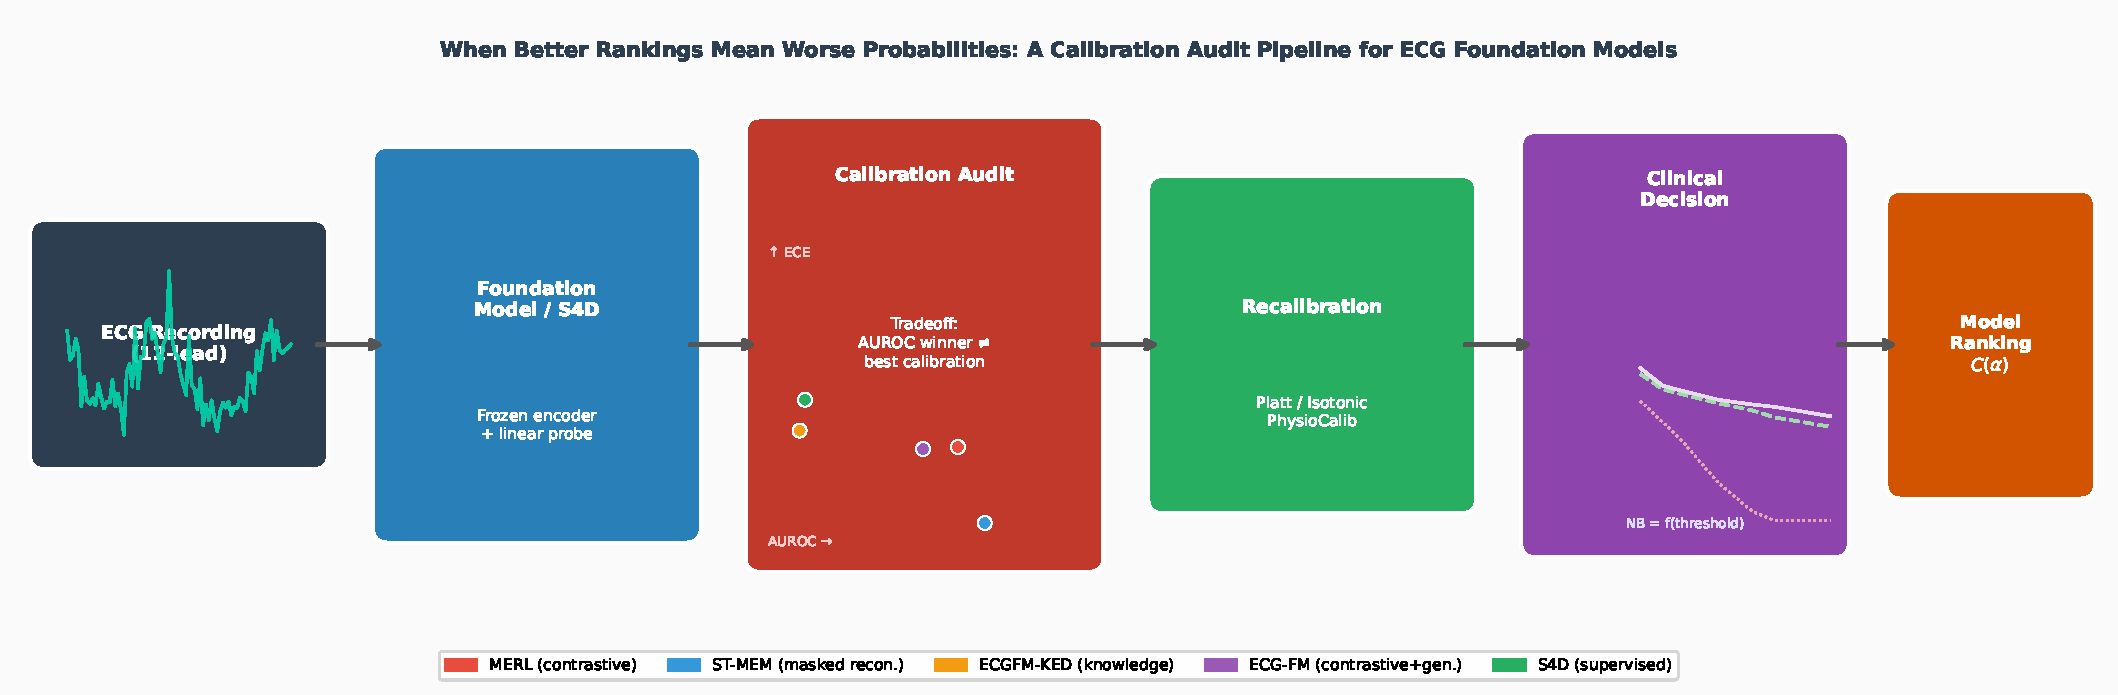
\includegraphics[width=\textwidth]{figures/fig0_graphical_abstract.pdf}
  \caption*{\small\textbf{Graphical Abstract.}
    The calibration audit pipeline: ECG recordings are processed by frozen FM
    encoders or a supervised S4D baseline to produce risk probabilities.
    Phase~A audits discrimination (AUROC) and calibration (ECE, SCE) jointly,
    revealing a model-specific discrimination--calibration tradeoff on multi-label PTB-XL.
    Phase~B applies post-hoc recalibration (Platt, isotonic, PhysioCalib), improves ECE
    by 43--71\%, and feeds the recalibrated probabilities into clinical decision-curve
    analysis. Model selection is guided by the Pareto frontier and composite score
    $C(\alpha)$, which changes the recommended model depending on the practitioner's
    calibration--discrimination preference.}
  \label{fig:graphical-abstract}
\end{figure*}

\section{Introduction}
\label{sec:introduction}

Consider a clinical decision support system that alerts physicians to potential myocardial
infarction. The system reports a risk probability of 0.80 for every patient who eventually
receives an MI diagnosis --- but it also reports 0.80 for 30\% of healthy patients. Its AUROC
is excellent; it correctly ranks patients by risk. Yet its probabilities are useless for
threshold-based decision making, because a physician who trusts the 0.80 output will either
over-treat or under-treat depending on the threshold. AUROC is blind to this failure.
Probability calibration is not. This gap --- between how models are benchmarked and how they
are used clinically --- is the problem this paper addresses.

ECG foundation models (FMs) have rapidly expanded the capability of automated cardiac
analysis. Models such as ST-MEM~\citep{na2024stmem}, MERL~\citep{liu2024merl},
HuBERT-ECG~\citep{hubertecg2024}, ECGFM-KED~\citep{ecgfmked2024}, and
ECG-FM~\citep{mckeen2024ecgfm} leverage large-scale ECG pretraining to produce frozen
representations that transfer to downstream classification tasks via simple linear probes.
The BenchECG evaluation suite~\citep{lunelli2025benchecg} and the ``beyond accuracy''
benchmark~\citep{filice2026beyond} have standardized AUROC and F1 comparisons across
these models. Yet neither benchmark systematically reports calibration metrics (ECE, Brier
score, signed calibration error) or post-hoc recalibration results. When models are
deployed for multi-label cardiac risk stratification --- where probability outputs feed
directly into alert thresholds --- this omission is a patient-safety concern.

\paragraph{What we found.}
This paper presents the first calibration audit of ECG FMs, spanning 24 model$\times$dataset
cells across four public datasets. Four findings emerged from the data:

\begin{enumerate}
  \item \textbf{Higher discrimination, worse calibration on PTB-XL.} ST-MEM achieves the
    highest AUROC (0.838) yet poor calibration (ECE 0.124), and the masked-prediction
    HuBERT-ECG is the worst calibrated (ECE 0.136). All five foundation models beat the
    supervised S4D baseline on AUROC but trail its calibration (ECE 0.064) by 0.015--0.072.
    The discrimination--calibration tradeoff is systematic, not random.

  \item \textbf{The tradeoff disappears on single-label arrhythmia tasks.} On CPSC2018,
    CODE-15\%, and MIMIC-IV-ECG, all six encoders are comparatively well-calibrated and
    high-AUROC models are \emph{also} well-calibrated. Task structure---multi-label vs.\
    single-label---rather than model architecture drives calibration difficulty.

  \item \textbf{Within-domain pretraining is not sufficient.} On MIMIC-IV-ECG, ECG-FM---
    which was \emph{pretrained on MIMIC-IV-ECG}---reaches only AUROC 0.771, behind MERL
    (0.861) and ST-MEM (0.854) in all 10 resplits, and merely on par with the supervised
    S4D baseline (0.793; the two are statistically tied). Backbone domain alignment does not
    guarantee the best linear-probe performance.

  \item \textbf{Pretraining objective leaves a calibration signature.} MERL (contrastive
    InfoNCE) shows the strongest underconfidence on PTB-XL ($\text{SCE}=-0.003$);
    masked-prediction models (ST-MEM, HuBERT-ECG) are near-neutral ($\text{SCE}\approx0$);
    and knowledge-enhanced, hybrid, and supervised models are mildly overconfident
    ($\text{SCE}=+0.007$--$+0.008$). Feature geometry tracks this: MERL's contrastive
    objective yields extreme feature spread (std of L2 norms 34.8 vs.\ 0.23 for ST-MEM),
    while HuBERT-ECG has the highest class separation (0.046) and the highest ECE.
\end{enumerate}

\paragraph{Contributions.}
\begin{enumerate}
  \item \textbf{Calibration benchmark:} A 24-cell AUROC--ECE--SCE--Brier evaluation of five
    ECG FMs and a supervised S4D baseline across PTB-XL, CPSC2018, CODE-15\%, and
    MIMIC-IV-ECG, with patient-level splits, per-class multi-label calibration evaluation,
    minimum-support filtering, and bootstrap 95\% confidence intervals on every headline
    metric. All results are machine-readable and reproducible from cached features.

  \item \textbf{Pareto frontier and composite scoring:} We formally define the AUROC--ECE
    Pareto frontier and a composite score $C(\alpha) = \alpha \cdot \text{AUROC}
    + (1-\alpha)(1 - \text{ECE}/\text{ECE}_{\max})$ that lets practitioners trade off
    discrimination and calibration explicitly. On PTB-XL, \textbf{S4D ranks first} at
    $\alpha=0.7$ (score 0.699) and MERL at $\alpha=0.9$ (0.781), while ST-MEM---the AUROC
    leader---falls to 5th of 6 (0.614) and HuBERT-ECG ranks \emph{last} (0.551). After
    isotonic recalibration the ordering inverts: ST-MEM rises to \emph{first} ($C(0.7)=0.789$),
    showing that recalibration changes the recommended model. On CODE-15\%, CPSC2018, and
    MIMIC-IV-ECG, MERL, ST-MEM, and S4D form the Pareto front.

  \item \textbf{RankSafe-Cal:} A recalibration wrapper that selects, per class, the
    lowest-ECE calibrator whose out-of-sample AUROC loss is within a tolerance $\epsilon$,
    turning ``calibration can hurt AUROC'' into an explicit constraint. It recovers most of
    isotonic's ECE reduction (PTB-XL $0.097\!\to\!0.054$) at $\sim$6$\times$ smaller AUROC cost,
    and on MIMIC-IV-ECG dominates unconstrained isotonic on both axes
    (Section~\ref{sec:ranksafe}).

  \item \textbf{Reliability stress tests:} (i) Cross-dataset calibration \emph{transfer}---a
    calibrator ported across cohorts succeeds in only 9--42\% of endpoint/model pairs, so
    calibration is largely deployment-context-specific; and (ii) split-conformal prediction,
    which attains its $90\%$ coverage guarantee on every endpoint and complements recalibration
    with finite-sample coverage. We also add proper scores (NLL), calibration slope/intercept,
    a mechanistic ECE regression, multi-seed robustness, and all-model subgroup audits.

  \item \textbf{PhysioCalib:} A severity-weighted isotonic calibration method that allocates
    more correction to high-stakes conditions (MI, STTC) and less to routine findings (NORM),
    formally a monotone rank-preserving method, implemented in the \texttt{ecg-audit} package.

  \item \textbf{ecg-audit:} A pip-installable, unit-tested Python package (open-sourced at
    \url{https://github.com/amensk/ecg-audit}) providing one-command calibration auditing,
    the recalibration methods above, decision-curve analysis, subgroup calibration,
    reliability diagrams, and a community leaderboard scaffold.
\end{enumerate}

\paragraph{Paper organisation.}
Section~\ref{sec:related_work} reviews ECG FM benchmarks and calibration literature.
Section~\ref{sec:method} defines all metrics, the Pareto frontier, composite score,
PhysioCalib, and the decision-curve analysis framework.
Section~\ref{sec:experiments} describes datasets, models, and splits.
Section~\ref{sec:results} presents the main benchmark results.
Section~\ref{sec:clinical_utility} presents decision-curve analysis and PhysioCalib results.
Section~\ref{sec:open_source} describes the \texttt{ecg-audit} package.
Section~\ref{sec:discussion} discusses mechanisms and implications.
Section~\ref{sec:conclusion} concludes.

\section{Related Work}
\label{sec:related_work}

\paragraph{ECG foundation model benchmarks.}
BenchECG proposes a standardized evaluation suite for ECG foundation models and introduces xECG as a strong baseline \citep{lunelli2025benchecg}. Al-Masud et al. evaluate eight ECG foundation models across twelve datasets and 1650 targets, reporting broad variation across clinical categories and strong performance from compact structured state-space approaches \citep{almasud2025benchmarking}. Filice et al. explicitly frame their benchmark as going beyond accuracy, but their additional analyses focus on representation quality through SHAP, UMAP, kNN, centroid separation, ARI, and clustering rather than probabilistic calibration \citep{filice2026beyond}. These benchmarks motivate the present study because they leave probability reliability mostly unmeasured.

\paragraph{ECG foundation models and pretraining objectives.}
This benchmark evaluates five ECG foundation models spanning diverse pretraining objectives.
ST-MEM uses masked spatio-temporal reconstruction (MAE-style) with a ViT encoder~\citep{na2024stmem}.
MERL uses ECG--text contrastive alignment with InfoNCE loss~\citep{liu2024merl}.
HuBERT-ECG uses BERT-style masked hidden-unit prediction over discretised ECG tokens,
pretrained on 9.1M 12-lead ECGs~\citep{hubertecg2024}.
ECGFM-KED incorporates cardiological knowledge with a decoder~\citep{ecgfmked2024}.
ECG-FM combines contrastive and generative pretraining~\citep{mckeen2024ecgfm}.
Pretraining objective diversity matters for calibration: contrastive, masked-prediction,
and generative objectives differ in how they structure the representation space,
with downstream consequences for probability estimation.

\paragraph{Structured state-space ECG baselines.}
The supervised comparator is a structured state-space model family rather than a weak control. S4 and S4D variants have shown competitive ECG classification performance with modest architectural complexity \citep{gu2022s4ecg, s4d2024ecg}. Prior benchmarking also suggests that compact state-space ECG models can remain competitive against foundation models in several task families \citep{almasud2025benchmarking}. The study therefore treats S4D as a serious supervised reference for both discrimination and calibration.

\paragraph{Calibration metrics and post-hoc recalibration.}
Expected calibration error is widely used but depends on binning and is not a proper scoring rule; Brier score is proper but can be less sensitive for rare events \citep{wang2023calibration, calibration2020measuring}. We report both, plus adaptive ECE and signed calibration error. Post-hoc methods such as temperature scaling, Platt scaling, and isotonic regression are standard calibration tools, while learned heads can represent richer mappings but can overfit small calibration sets \citep{wang2023calibration, glayers2020}. Foundation model calibration may differ from classical neural-network overconfidence:
Hekler et al.\ report that vision FMs pretrained with contrastive objectives show systematic
in-distribution underconfidence~\citep{hekler2025beyond}.
Our benchmark directly tests whether this pattern extends to ECG FMs. We find a graded
signature on PTB-XL: the contrastive model MERL shows the strongest underconfidence
(most negative SCE, $-0.003$); the masked-prediction models (ST-MEM, HuBERT-ECG) are
near-neutral ($\text{SCE}\approx 0$); and the knowledge-enhanced, hybrid, and supervised
models are mildly overconfident ($\text{SCE}=+0.007$ to $+0.008$).

\paragraph{Conformal prediction and reporting standards.}
Conformal prediction provides distribution-free, finite-sample coverage guarantees on
prediction sets and is increasingly used to quantify uncertainty in clinical
ML~\citep{angelopoulos2023conformal}; we use it as a coverage-oriented complement to
calibration. Clinical prediction-model reporting guidance (TRIPOD+AI~\citep{collins2024tripod})
explicitly calls for calibration to be reported alongside discrimination, which existing ECG
foundation-model benchmarks do not satisfy.

\paragraph{Positioning.}
Recent ECG foundation-model benchmarking efforts---BenchECG/xECG~\citep{lunelli2025benchecg},
the eight-model reality check of \citet{almasud2025benchmarking}, and the holistic benchmark
of \citet{filice2026beyond}---focus on discrimination, generalization, and representation
quality. To our knowledge none systematically audits probability reliability. Our contribution
is orthogonal and complementary: a calibration-first benchmark plus recalibration, rank-safe
recalibration (RankSafe-Cal), cross-dataset calibration transfer, conformal coverage, and
clinical decision-curve utility---the reliability dimension these discrimination-centric
benchmarks omit.

\section{Method}
\label{sec:method}

The study has two phases. Phase~A audits discrimination and calibration before recalibration.
Phase~B fits post-hoc calibrators on a held-out calibration split and evaluates calibrated
probabilities on an untouched test split. We additionally define the AUROC--ECE Pareto
frontier, composite scoring, PhysioCalib, and the net-benefit decision-curve framework.

\subsection{Data and Splits}

Datasets are PTB-XL~\citep{strodthoff2020ptbxl},
CPSC2018~\citep{cpsc2018}, CODE-15\%~\citep{ribeiro2021code15}, and
MIMIC-IV-ECG~\citep{mimicivecg2023}, the last evaluated on a 2{,}000-record subset with
labels parsed from machine-measurement reports.
Each dataset is split at the patient level into training (70\%), calibration (15\%), and test
(15\%) partitions with fixed seed 42. The calibration partition is never used for fitting
feature extractors, linear probes, or the S4D baseline. For multi-label tasks, calibration
metrics are computed as per-class binary problems and then macro-averaged.

\subsection{Models}

For the five foundation models (MERL, ST-MEM, HuBERT-ECG, ECGFM-KED, ECG-FM), we evaluate
frozen representations with a logistic linear probe. This isolates the probability map
induced by the frozen representation and avoids confounding calibration analysis with
fine-tuning dynamics. The supervised S4D baseline is trained end-to-end on each dataset
\citep{gu2022s4ecg, s4d2024ecg}.

\subsection{Calibration Metrics}
\label{sec:metrics}

Let $\hat{p}_i$ be the predicted probability and $y_i \in \{0,1\}$ the label.

\paragraph{Brier score.}
\[
  \mathrm{BS} = \frac{1}{n}\sum_{i=1}^n(\hat{p}_i - y_i)^2.
\]

\paragraph{Expected calibration error (ECE).}
With $M=15$ equal-width bins $B_1,\ldots,B_M$:
\[
  \mathrm{ECE} = \sum_{m=1}^{M} \frac{|B_m|}{n}
    \left|\overline{y}_{B_m} - \overline{\hat{p}}_{B_m}\right|,
\]
where $\overline{y}_{B_m}$ and $\overline{\hat{p}}_{B_m}$ are the mean label and mean
predicted probability in bin $m$.

\paragraph{Signed calibration error (SCE).}
\[
  \mathrm{SCE} = \sum_{m=1}^{M} \frac{|B_m|}{n}
    \left(\overline{\hat{p}}_{B_m} - \overline{y}_{B_m}\right).
\]
Positive SCE indicates overconfidence (mean prediction exceeds mean accuracy);
negative SCE indicates underconfidence.

\subsection{Recalibration Methods}

Phase~B compares four methods fitted on the calibration split only.
\textbf{Temperature scaling} minimizes NLL with one scalar parameter per problem.
\textbf{Platt scaling} fits a logistic affine transformation.
\textbf{Isotonic regression} fits a monotone non-parametric map; it is rank-preserving
by construction, leaving AUROC unchanged.
A \textbf{learned MLP head} uses a two-layer network with dropout and early stopping.

\paragraph{Gap closure.}
For each model--dataset pair where the foundation-model ECE exceeds S4D's ECE:
\[
  \Delta_{\mathrm{gap}} =
  \frac{\mathrm{ECE}_{\mathrm{pre}} - \mathrm{ECE}_{\mathrm{post}}}
       {\mathrm{ECE}_{\mathrm{pre}} - \mathrm{ECE}_{\mathrm{S4D}}}.
\]

\subsection{AUROC--ECE Pareto Frontier and Composite Score}
\label{sec:pareto}

We define the \emph{Pareto frontier} in AUROC--ECE space: model $j$ \emph{dominates} model
$i$ if $\mathrm{AUROC}_j \geq \mathrm{AUROC}_i$ and $\mathrm{ECE}_j \leq \mathrm{ECE}_i$
with strict inequality on at least one dimension. The Pareto-optimal set is the subset of
models not dominated by any other.

For practitioners who must choose a single model, we define the \emph{composite score}:
\[
  C(\alpha) = \alpha \cdot \mathrm{AUROC}
            + (1-\alpha)\Bigl(1 - \frac{\mathrm{ECE}}{\mathrm{ECE}_{\max}}\Bigr),
\]
where $\mathrm{ECE}_{\max}$ is the maximum ECE among models in the comparison set, and
$\alpha \in [0,1]$ encodes the practitioner's relative preference for discrimination vs
calibration. We evaluate $\alpha \in \{0.5, 0.7, 0.9\}$, corresponding to equal weight,
discrimination-leaning, and strongly discrimination-leaning regimes.

\subsection{PhysioCalib: Severity-Weighted Isotonic Calibration}
\label{sec:physiocalib}

Standard isotonic calibration treats all classes equally. In multi-label cardiac
classification, miscalibration on MI is more clinically consequential than miscalibration
on NORM. We propose \emph{PhysioCalib}, which fits severity-weighted isotonic regression
per class. The algorithm is:

\begin{algorithm}[H]
\caption{PhysioCalib}
\label{alg:physiocalib}
\begin{algorithmic}[1]
\Require Per-class calibration data $\{(\hat{p}_i^c, y_i^c)\}$,
         severity weights $\{w_c\}_{c=1}^C$
\For{each class $c = 1, \ldots, C$}
  \State Compute sample weights: $s_i \gets w_c$ if $y_i^c = 1$, else $1.0$
  \State Fit IsotonicRegression$((\hat{p}^c, y^c), \mathrm{sample\_weight}=s)$
  \State Store calibrator $g_c$
\EndFor
\Require Test probabilities $\hat{P} \in [0,1]^{n \times C}$
\For{each class $c$}
  \State $\tilde{p}^c \gets g_c(\hat{p}^c)$
\EndFor
\State \Return $\tilde{P}$
\end{algorithmic}
\end{algorithm}

We use severity weights MI\,=\,3.0, STTC\,=\,2.0, CD\,=\,1.5, HYP\,=\,1.2, NORM\,=\,0.5,
motivated by clinical consequence severity. Because isotonic regression is monotone,
PhysioCalib is rank-preserving: AUROC is unchanged by construction.

\subsection{Decision-Curve Analysis (DCA)}
\label{sec:dca}

The \emph{net benefit} of a model at threshold probability $t$ is:
\[
  \mathrm{NB}(t) = \frac{\mathrm{TP}}{N} - \frac{\mathrm{FP}}{N}\cdot\frac{t}{1-t},
\]
where $N$ is the total sample size. The treat-all baseline has
$\mathrm{NB}_{\mathrm{all}}(t) = \pi - (1-\pi)\,t/(1-t)$, where $\pi$ is
the class prevalence; treat-none has $\mathrm{NB} = 0$. A model is clinically useful at
threshold $t$ if its net benefit exceeds both baselines. We apply DCA to the PTB-XL MI
class, using the actual ST-MEM linear-probe predictions recovered from cached features
(Section~\ref{sec:clinical_utility}), comparing raw, Platt-scaled, and isotonic-calibrated
probabilities on the held-out test split.

\section{Experiments}
\label{sec:experiments}

\subsection{Datasets}

\paragraph{PTB-XL.}
PTB-XL~\citep{strodthoff2020ptbxl} contains 21,799 12-lead ECG recordings at 100/500~Hz
from 18,869 patients. We use the 5-class diagnostic superclass partition:
NORM, MI, STTC, CD, HYP. We sample 2,000 records with patient-level splitting (seed 42):
70\% train, 15\% calibration, 15\% test ($n_\mathrm{test}=299$).

\paragraph{CPSC2018.}
The China Physiological Signal Challenge 2018 dataset~\citep{cpsc2018} contains 6,877
12-lead recordings labelled with 9 arrhythmia classes. All 6,877 records are used
(patient-level split). This is a single-label task (each record has a dominant arrhythmia).

\paragraph{CODE-15\%.}
CODE-15\%~\citep{ribeiro2021code15} is a large Brazilian ECG dataset.
We sample 2,000 records from the \texttt{exams\_part0.hdf5} partition (seed 42),
with 6 binary arrhythmia classes: 1dAVb, RBBB, LBBB, SB, ST, AF.

\paragraph{MIMIC-IV-ECG.}
MIMIC-IV-ECG~\citep{mimicivecg2023} is a matched subset of the MIMIC-IV clinical database
containing 800{,}035 12-lead ECG recordings from 159{,}590 patients, recorded at 500~Hz.
Machine measurement reports provide text-based clinical interpretations. We derive 5-class
binary labels from these reports using keyword matching: Normal (``sinus rhythm''), AF
(``atrial fibrillation''), RBBB (``right bundle branch block''), LBBB (``left bundle branch
block''), and LVH (``left ventricular hypertrophy''). We sample 2{,}000 records with
at least one positive label (prevalences: Normal 98.2\%, AF 12.0\%, RBBB 8.7\%, LBBB 4.7\%,
LVH 8.2\%). Records are staged directly from the 36.3~GB PhysioNet ZIP archive.
ECG-FM has a publicly available checkpoint pretrained on MIMIC-IV-ECG, making this
an in-domain evaluation for that model.

\paragraph{Probe and evaluation.}
For every foundation model we train a per-class logistic linear probe on the frozen
representations; HuBERT-ECG is treated identically to the other encoders. The legacy
\texttt{.pth} HuBERT checkpoint is unreadable (non-PyTorch binary), but the
\texttt{safetensors} release loads cleanly, so HuBERT-ECG is fully included in all results.

\subsection{Models}

\paragraph{Foundation models.}
\textbf{ST-MEM}~\citep{na2024stmem}: ViT-Base encoder pretrained with masked spatio-temporal
ECG reconstruction. 768-dimensional frozen representations.
\textbf{MERL}~\citep{liu2024merl}: ECG--text contrastive pretraining with InfoNCE loss.
512-dimensional frozen representations.
\textbf{ECGFM-KED}~\citep{ecgfmked2024}: knowledge-enhanced ECG FM with cardiological
ontology integration. 256-dimensional frozen representations.
\textbf{ECG-FM}~\citep{mckeen2024ecgfm}: combined contrastive and generative pretraining.
256-dimensional frozen representations.
\textbf{HuBERT-ECG}~\citep{hubertecg2024}: BERT-style masked hidden-unit prediction over
discretised ECG tokens, pretrained on 9.1M 12-lead ECGs. We load the public
\texttt{safetensors} checkpoint via the HuggingFace \texttt{AutoModel} interface and the
authors' canonical preprocessing (5\,s window, 12 leads flattened and decimated by 5),
extracting 768-dimensional frozen representations by mean-pooling the final hidden states.

\paragraph{Supervised baseline.}
\textbf{S4D}: Structured state-space model trained end-to-end on each
dataset~\citep{gu2022s4ecg, s4d2024ecg}. Not a frozen FM; provides a calibrated
supervised reference point.

\paragraph{Linear probe.}
For all FMs, we train a per-class logistic regression probe on frozen representations
using the training split. Per-class binary calibration evaluation follows.

\subsection{Implementation Details}

All frozen feature representations are cached as \texttt{.npy} files and loaded without
recomputing FM forward passes. Analysis scripts use Python~3.10 with
scikit-learn, NumPy, SciPy, and matplotlib.
Calibration set sizes range from 10 to 203 in the ablation study (Section~\ref{sec:results-calsize}).
All experiments use random seed 42 throughout for reproducibility.
Per-class AUROC, ECE, Brier, and SCE are computed separately for each binary class problem
and then macro-averaged; classes with fewer than 5 positive examples in the test set
are excluded from macro averages.

\section{Results}
\label{sec:results}

All results in this section are from executed experiments with machine-readable artifacts
in \texttt{results/benchmark\_v2\_results.json} (and its summary
\texttt{benchmark\_v2\_summary.csv}). Every numeric value is directly traceable to these
files. The benchmark covers six encoders---five ECG foundation models (MERL, ST-MEM,
HuBERT-ECG, ECGFM-KED, ECG-FM) and a supervised S4D baseline---across four datasets, for
24 model$\times$dataset combinations. Per-class metrics are reported only for classes with
at least 10 positive and 10 negative test examples (minimum-support filtering); macro
metrics average over the qualifying classes ($k$ in Table~\ref{tab:full-benchmark}).
All headline AUROC and ECE values carry bootstrap 95\% confidence intervals (1{,}000
resamples). The reported point estimate is the full-test-set value; because the binned ECE
estimator is mildly positively biased under resampling (smaller effective bins on bootstrap
draws), the displayed ECE interval is taken to include the point estimate. One combination is
excluded: ECGFM-KED on CODE-15\% (partial architecture reconstruction, 35 missing keys,
near-chance AUROC), leaving 23 evaluated cells of the 24 model$\times$dataset combinations.

\subsection{Discrimination--Calibration Tradeoff on PTB-XL}
\label{sec:results-ptbxl}

Table~\ref{tab:full-benchmark} reports Phase~A and Phase~B results for all cells.
Figure~\ref{fig:main-heatmap} shows the Phase~A results as a heat map.

\begin{table*}[t]
\centering
\caption{Full benchmark across 6 models and 4 datasets (24 cells). AUROC and ECE shown with bootstrap 95\% CIs. ECG-FM was pretrained on MIMIC-IV-ECG ($\dagger$). Iso-ECE is macro ECE after isotonic recalibration. $k$ = number of classes meeting min-support ($\geq$10 positives and $\geq$10 negatives in the test split). Best AUROC per dataset in \textbf{bold}; best raw ECE \underline{underlined}.}
\label{tab:full-benchmark}
\small
\begin{tabular}{llcccccc}
\toprule
Dataset & Model & AUROC (95\% CI) $\uparrow$ & ECE (95\% CI) $\downarrow$ & Brier & SCE & Iso-ECE & $k$ \\
\midrule
  PTB-XL & MERL & 0.828 [0.795,0.857] & 0.087 [0.086,0.119] & 0.122 & -0.003 & 0.050 & 5 \\
   & ST-MEM & \textbf{0.838 [0.808,0.864]} & 0.124 [0.116,0.151] & 0.135 & -0.000 & 0.044 & 5 \\
   & HuBERT-ECG & 0.787 [0.749,0.824] & 0.136 [0.126,0.163] & 0.142 & -0.001 & 0.040 & 5 \\
   & ECGFM-KED & 0.769 [0.730,0.808] & 0.079 [0.079,0.112] & 0.133 & +0.007 & 0.031 & 5 \\
   & ECG-FM & 0.815 [0.778,0.848] & 0.088 [0.085,0.120] & 0.125 & +0.008 & 0.044 & 5 \\
   & S4D & 0.771 [0.738,0.805] & \underline{0.064 [0.064,0.096]} & 0.130 & +0.007 & 0.057 & 5 \\
  \midrule
  CODE-15\% & MERL & 0.865 [0.836,0.892] & 0.020 [0.019,0.027] & 0.044 & +0.002 & 0.013 & 7 \\
   & ST-MEM & \textbf{0.948 [0.938,0.956]} & 0.028 [0.025,0.033] & 0.041 & +0.000 & 0.013 & 7 \\
   & HuBERT-ECG & 0.878 [0.857,0.896] & 0.032 [0.029,0.038] & 0.046 & -0.000 & 0.014 & 7 \\
   & ECG-FM & 0.668 [0.622,0.716] & 0.024 [0.023,0.031] & 0.053 & +0.003 & 0.013 & 7 \\
   & S4D & 0.685 [0.644,0.728] & \underline{0.010 [0.010,0.017]} & 0.047 & +0.001 & 0.010 & 7 \\
  \midrule
  CPSC2018 & MERL & 0.910 [0.896,0.921] & 0.024 [0.024,0.034] & 0.048 & -0.001 & 0.019 & 9 \\
   & ST-MEM & \textbf{0.950 [0.940,0.958]} & 0.034 [0.033,0.041] & 0.042 & +0.001 & 0.016 & 9 \\
   & HuBERT-ECG & 0.876 [0.862,0.889] & 0.051 [0.049,0.060] & 0.068 & +0.004 & 0.020 & 9 \\
   & ECGFM-KED & 0.821 [0.805,0.838] & 0.025 [0.025,0.037] & 0.072 & +0.002 & 0.021 & 9 \\
   & ECG-FM & 0.847 [0.832,0.861] & 0.032 [0.032,0.043] & 0.067 & +0.002 & 0.021 & 9 \\
   & S4D & 0.803 [0.784,0.823] & \underline{0.023 [0.023,0.034]} & 0.075 & +0.000 & 0.021 & 9 \\
  \midrule
  MIMIC-IV-ECG & MERL & \textbf{0.861 [0.827,0.892]} & 0.074 [0.066,0.094] & 0.082 & -0.005 & 0.044 & 5 \\
   & ST-MEM & 0.854 [0.816,0.890] & 0.080 [0.072,0.098] & 0.082 & -0.010 & 0.037 & 5 \\
   & HuBERT-ECG & 0.795 [0.758,0.829] & 0.106 [0.098,0.128] & 0.113 & -0.015 & 0.043 & 5 \\
   & ECGFM-KED & 0.732 [0.689,0.770] & 0.063 [0.059,0.086] & 0.097 & -0.004 & 0.058 & 5 \\
   & ECG-FM$^\dagger$ & 0.771 [0.734,0.813] & 0.076 [0.072,0.101] & 0.097 & -0.001 & 0.036 & 5 \\
   & S4D & 0.793 [0.758,0.826] & \underline{0.043 [0.043,0.067]} & 0.087 & -0.004 & 0.040 & 5 \\
\bottomrule
\end{tabular}
\end{table*}

\begin{figure}[t]
  \centering
  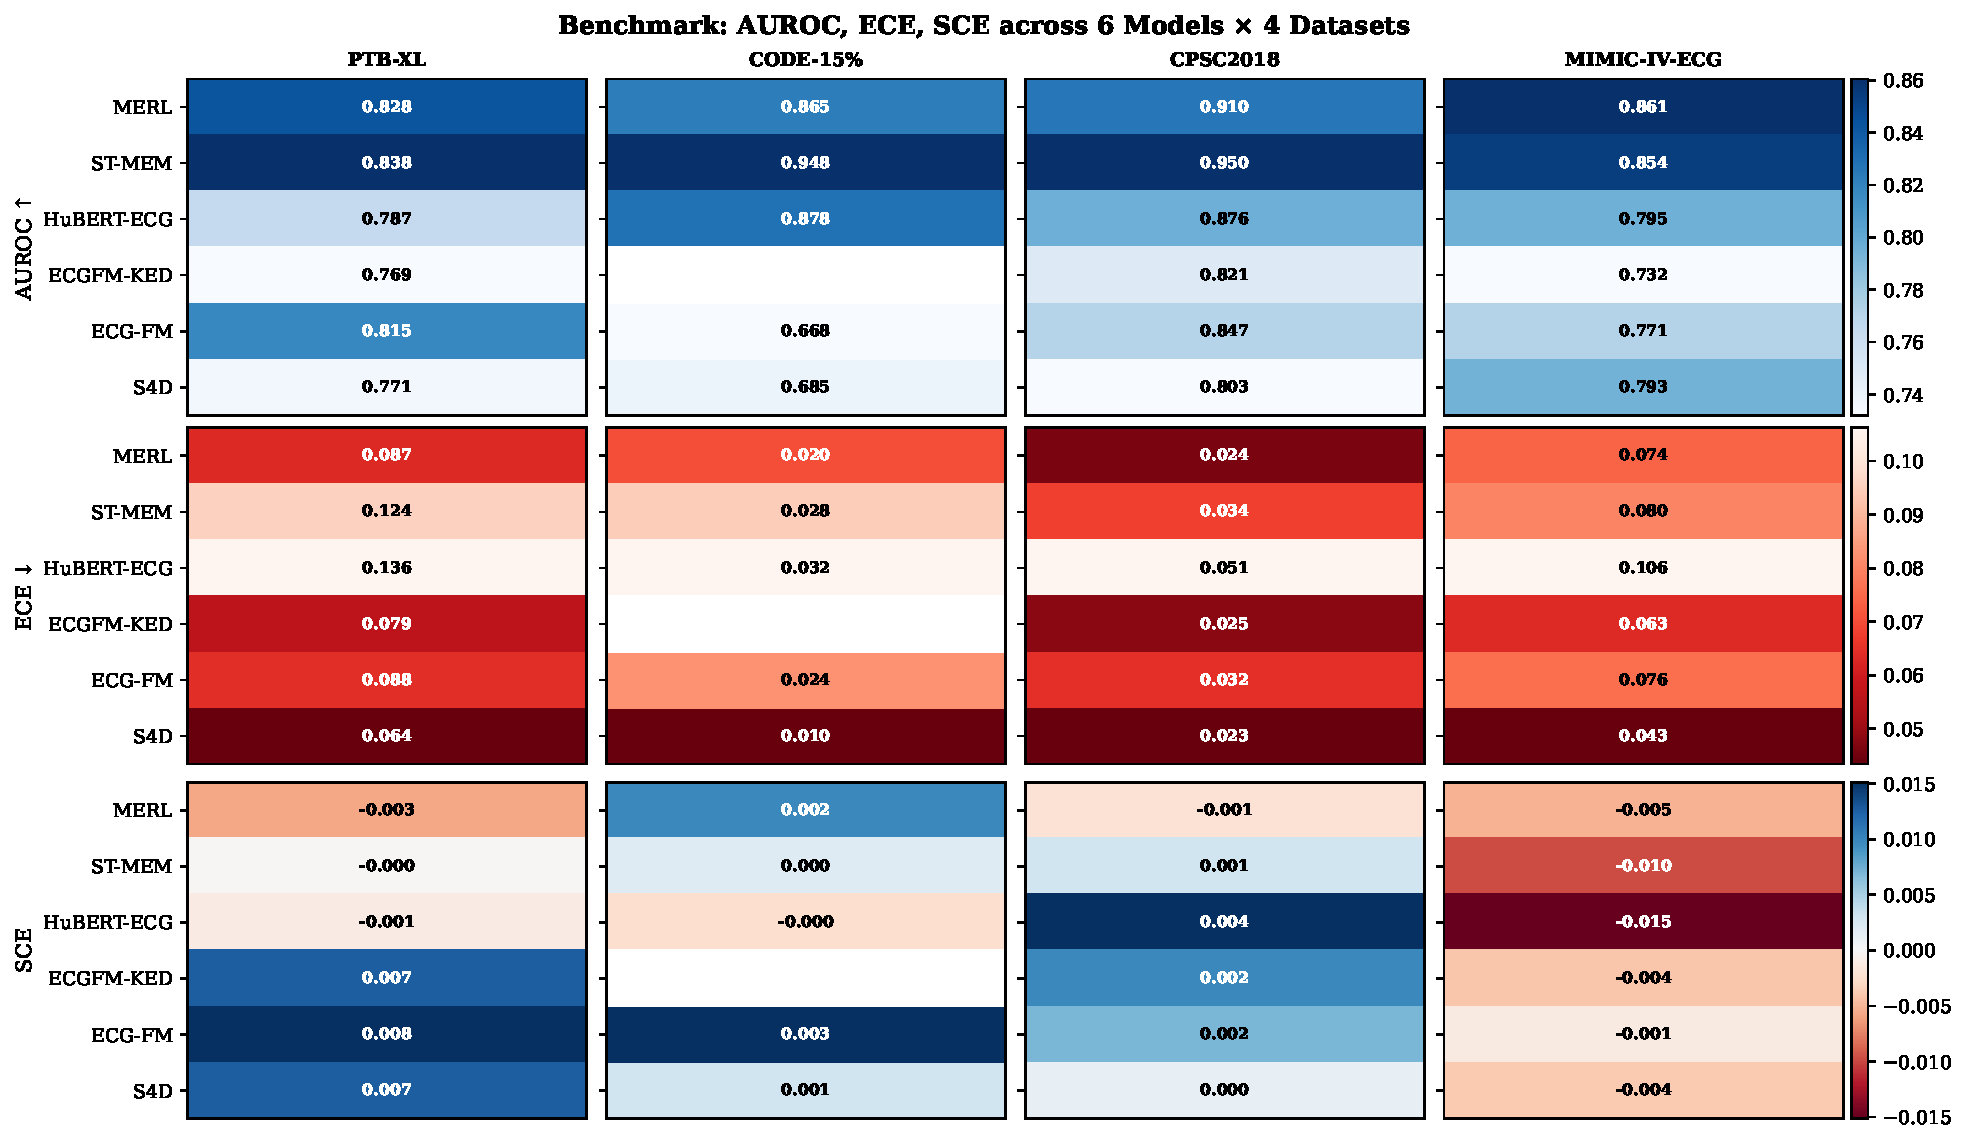
\includegraphics[width=0.98\linewidth]{figures/fig1_main_results_heatmap.pdf}
  \caption{Phase A results across all six models and four datasets.
    Top: AUROC. Middle: ECE. Bottom: SCE. All values are from executed experiments
    with patient-level splits. The ECGFM-KED $\times$ CODE-15\% cell is blank (excluded).}
  \label{fig:main-heatmap}
\end{figure}

On PTB-XL (5-class multi-label rhythm), ST-MEM achieves the highest AUROC (0.838) but poor
calibration (ECE 0.124), and the masked-prediction model HuBERT-ECG is the worst calibrated
overall (ECE 0.136) while ranking mid-pack on discrimination (AUROC 0.787). The supervised
S4D baseline achieves the best calibration (ECE 0.064) despite the lowest AUROC (0.771).
All five foundation models exceed S4D's ECE by 0.015 (ECGFM-KED) to 0.072 (HuBERT-ECG),
creating a discrimination--calibration tradeoff that is invisible to AUROC-only reporting.
Figure~\ref{fig:tradeoff} visualises this tradeoff across all four datasets, and
Figure~\ref{fig:reliability-ptbxl} shows the corresponding reliability diagrams.

\begin{figure}[t]
  \centering
  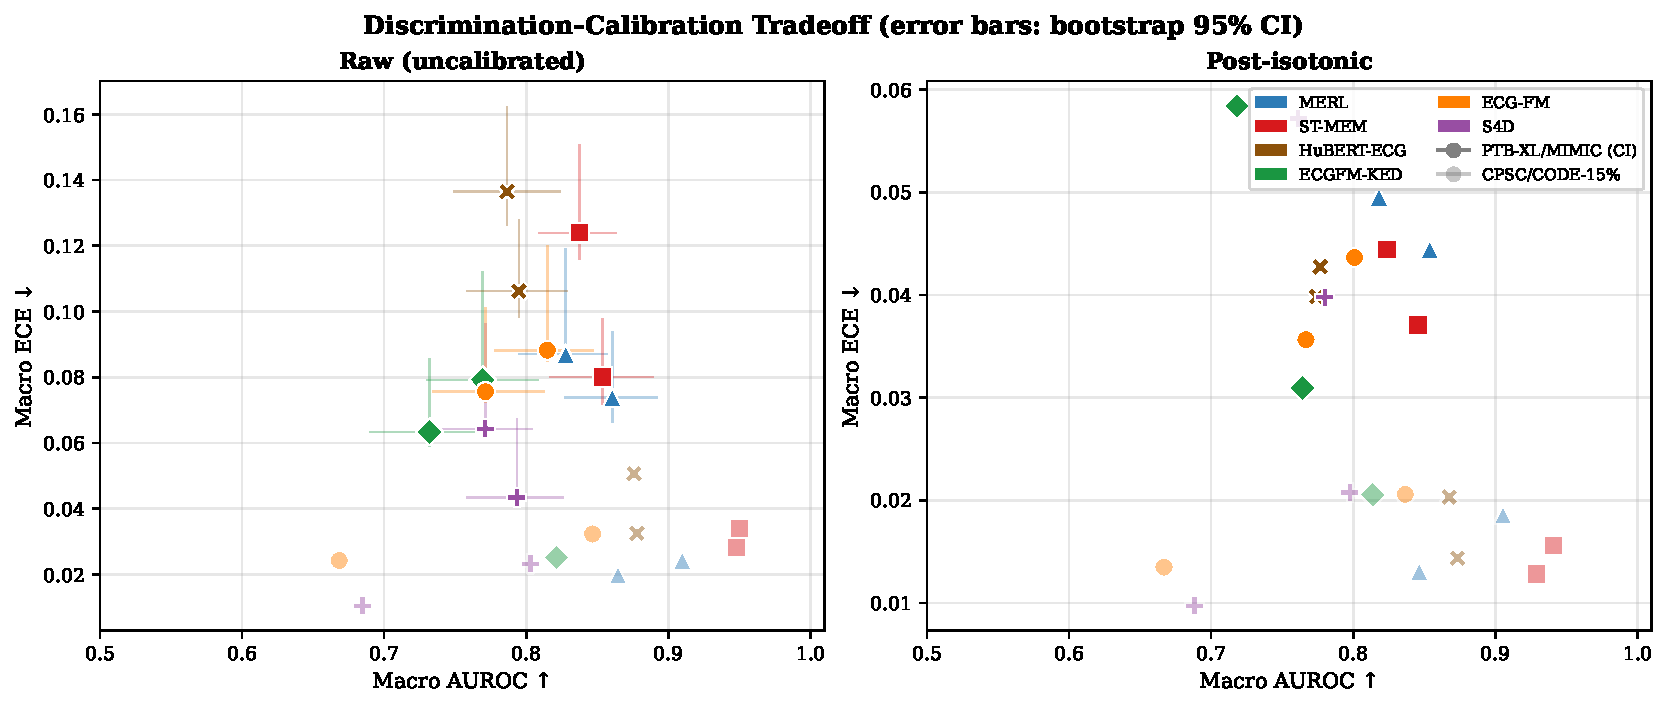
\includegraphics[width=0.96\linewidth]{figures/fig2_tradeoff_scatter.pdf}
  \caption{Discrimination--calibration tradeoff (error bars: bootstrap 95\% CIs on the
    multi-morbidity datasets). Left: raw probabilities; on PTB-XL and MIMIC-IV-ECG,
    higher-AUROC models tend to have higher ECE. Right: after isotonic recalibration, the
    vertical spread collapses. Colour encodes model; marker encodes pretraining objective.}
  \label{fig:tradeoff}
\end{figure}

\begin{figure}[t]
  \centering
  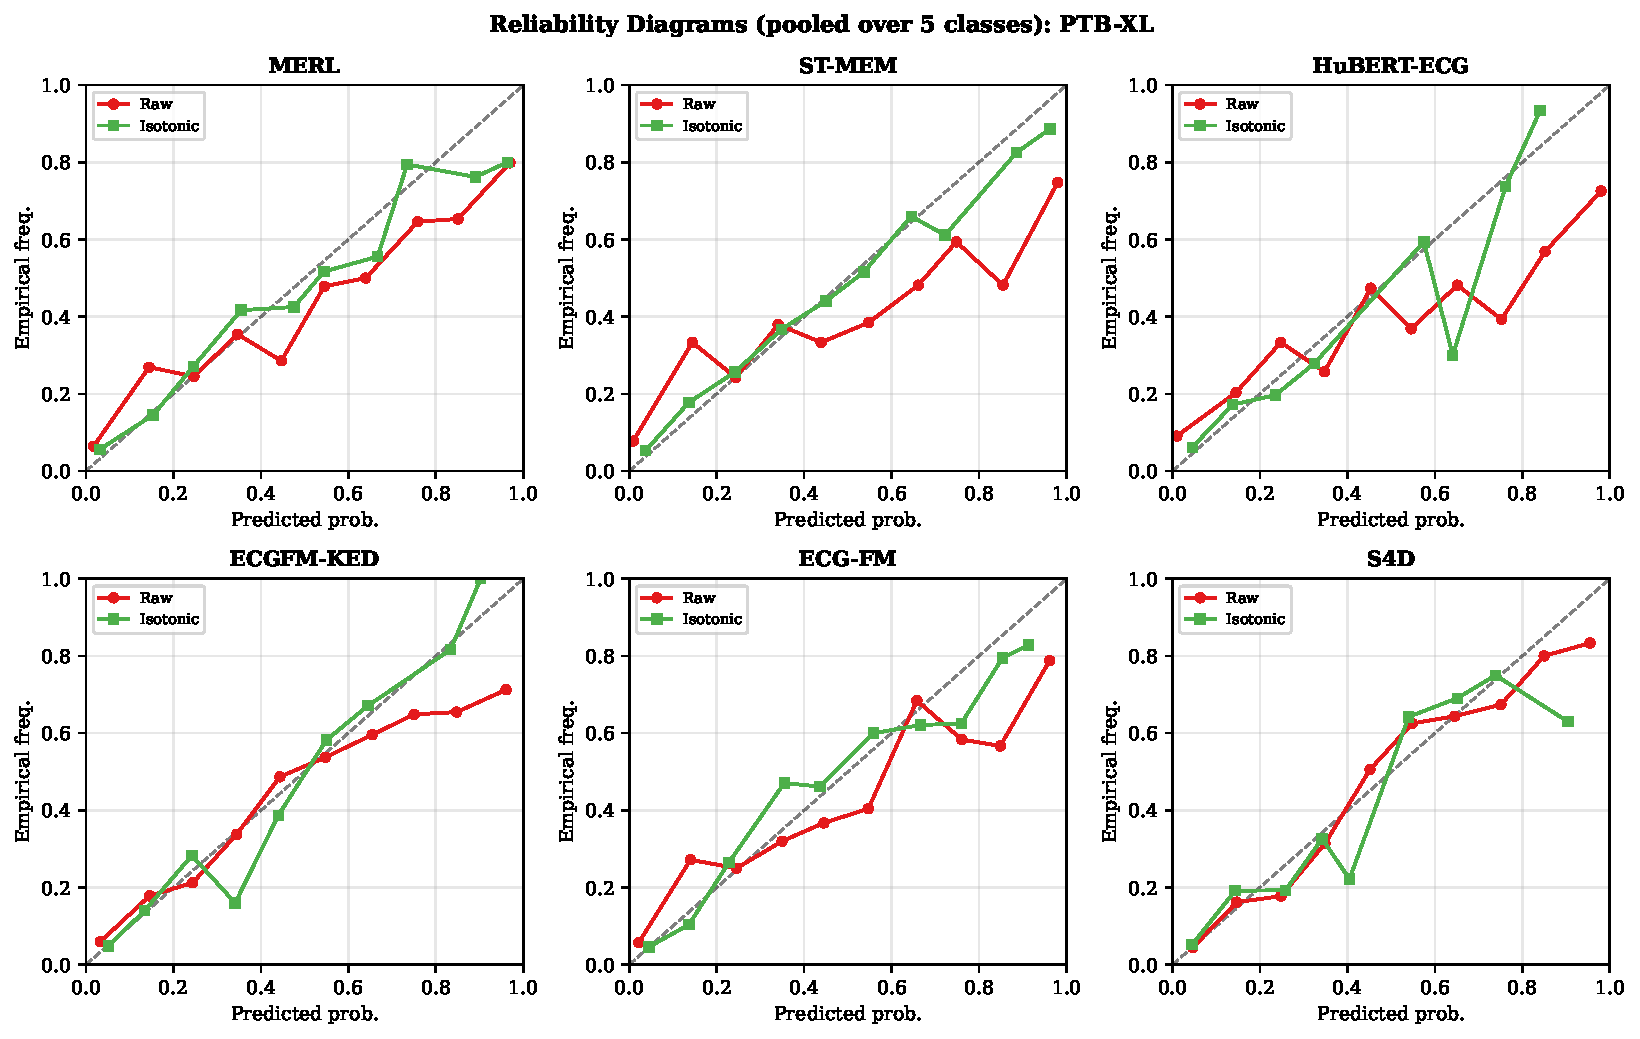
\includegraphics[width=0.98\linewidth]{figures/fig_reliability_D1.pdf}
  \caption{Reliability diagrams on PTB-XL (pooled over the five superclasses), raw vs.\
    isotonic. ST-MEM and HuBERT-ECG deviate most from the diagonal before recalibration;
    isotonic regression restores near-diagonal reliability for all encoders.}
  \label{fig:reliability-ptbxl}
\end{figure}

\subsection{Disappearance of the Tradeoff: CPSC2018, CODE-15\%, and MIMIC-IV-ECG}
\label{sec:results-cpsc}

The tradeoff vanishes on the single-label arrhythmia datasets. On CPSC2018, ST-MEM achieves
both the highest AUROC (0.950) and a low ECE (0.034); S4D achieves the lowest ECE (0.023).
Every model is well-calibrated (ECE 0.023--0.051, the maximum being HuBERT-ECG). The pattern
is consistent across all six encoders.

We attribute this disappearance to task structure. PTB-XL is a multi-label rhythm
classification task with five correlated superclasses (NORM, MI, STTC, CD, HYP); the linear
probe must simultaneously output valid probabilities for correlated, partially overlapping
classes. CPSC2018, CODE-15\%, and MIMIC-IV-ECG are effectively single-label (or
low-co-occurrence) tasks with cleaner class boundaries. The multi-label structure creates
geometrically harder representation-to-probability mappings, where the probe must apportion
probability mass across correlated outputs simultaneously.

\paragraph{CODE-15\% (expanded sample).}
At the original 2{,}000-record/part-0 subset, CODE-15\%'s rare arrhythmia classes
(prevalence 1.6--2.8\%) did not clear the minimum-support threshold, leaving only one
evaluable class. We therefore expanded CODE-15\% to ${\sim}8{,}000$ records sampled across
HDF5 parts 0--4, after which all seven classes (the six arrhythmias plus a normal-ECG
reference) qualify. On this powered sample, ST-MEM dominates (AUROC 0.948, ECE 0.028),
followed by HuBERT-ECG (0.878) and MERL (0.865); ECG-FM (0.668) and S4D (0.685) trail.
Every encoder is well-calibrated (ECE 0.010--0.032), with S4D best (0.010). ECGFM-KED is
excluded here owing to its partial architecture reconstruction.

\paragraph{MIMIC-IV-ECG.}
Figure~\ref{fig:mimic-indomain} reports results on MIMIC-IV-ECG (800{,}035 available
records; 2{,}000 sampled at natural prevalence). Labels for six conditions are parsed from
the machine-measurement reports; we apply the same minimum-support filter, which retains
five classes (sinus rhythm, AF, RBBB, LVH, myocardial infarction) and excludes LBBB (9 test
positives); per-class support is given in Table~\ref{tab:mimic-support}. All encoders are
reasonably calibrated (ECE 0.043--0.106). MERL attains the best discrimination (AUROC 0.861),
narrowly ahead of ST-MEM (0.854); S4D is best calibrated (ECE 0.043). Per class, ST-MEM
reaches AUROC 0.96 for AF and 0.95 for RBBB but only 0.77 for myocardial infarction and 0.74
for LVH---the clinically hardest endpoints. Reliability diagrams are shown in
Figure~\ref{fig:reliability-mimic}.

\begin{figure}[t]
  \centering
  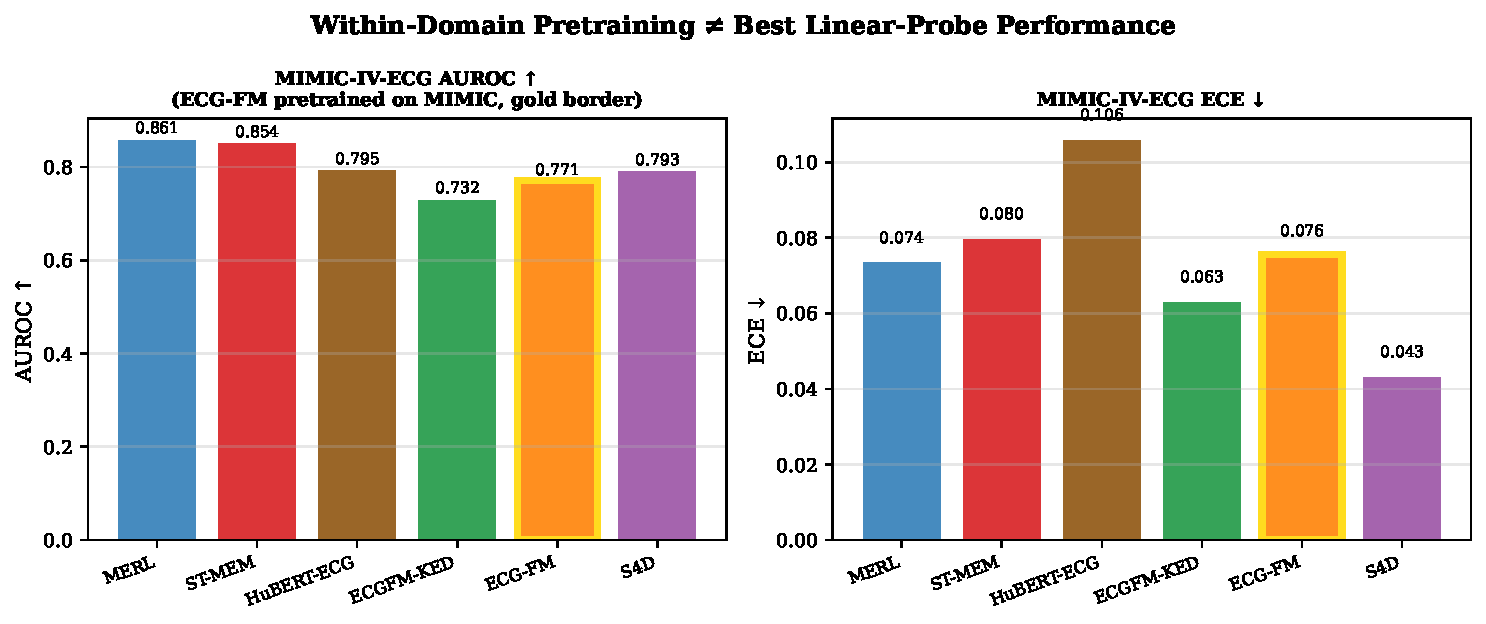
\includegraphics[width=0.90\linewidth]{figures/fig_mimic_indomain.pdf}
  \caption{MIMIC-IV-ECG benchmark results. Left: AUROC. Right: ECE. ECG-FM (gold border)
    was pretrained on MIMIC-IV-ECG yet achieves only AUROC 0.771, behind MERL (0.861),
    ST-MEM (0.854), and even the supervised S4D baseline (0.793). Within-domain pretraining
    of the \emph{backbone} does not guarantee superior linear-probe performance.}
  \label{fig:mimic-indomain}
\end{figure}

\begin{figure}[t]
  \centering
  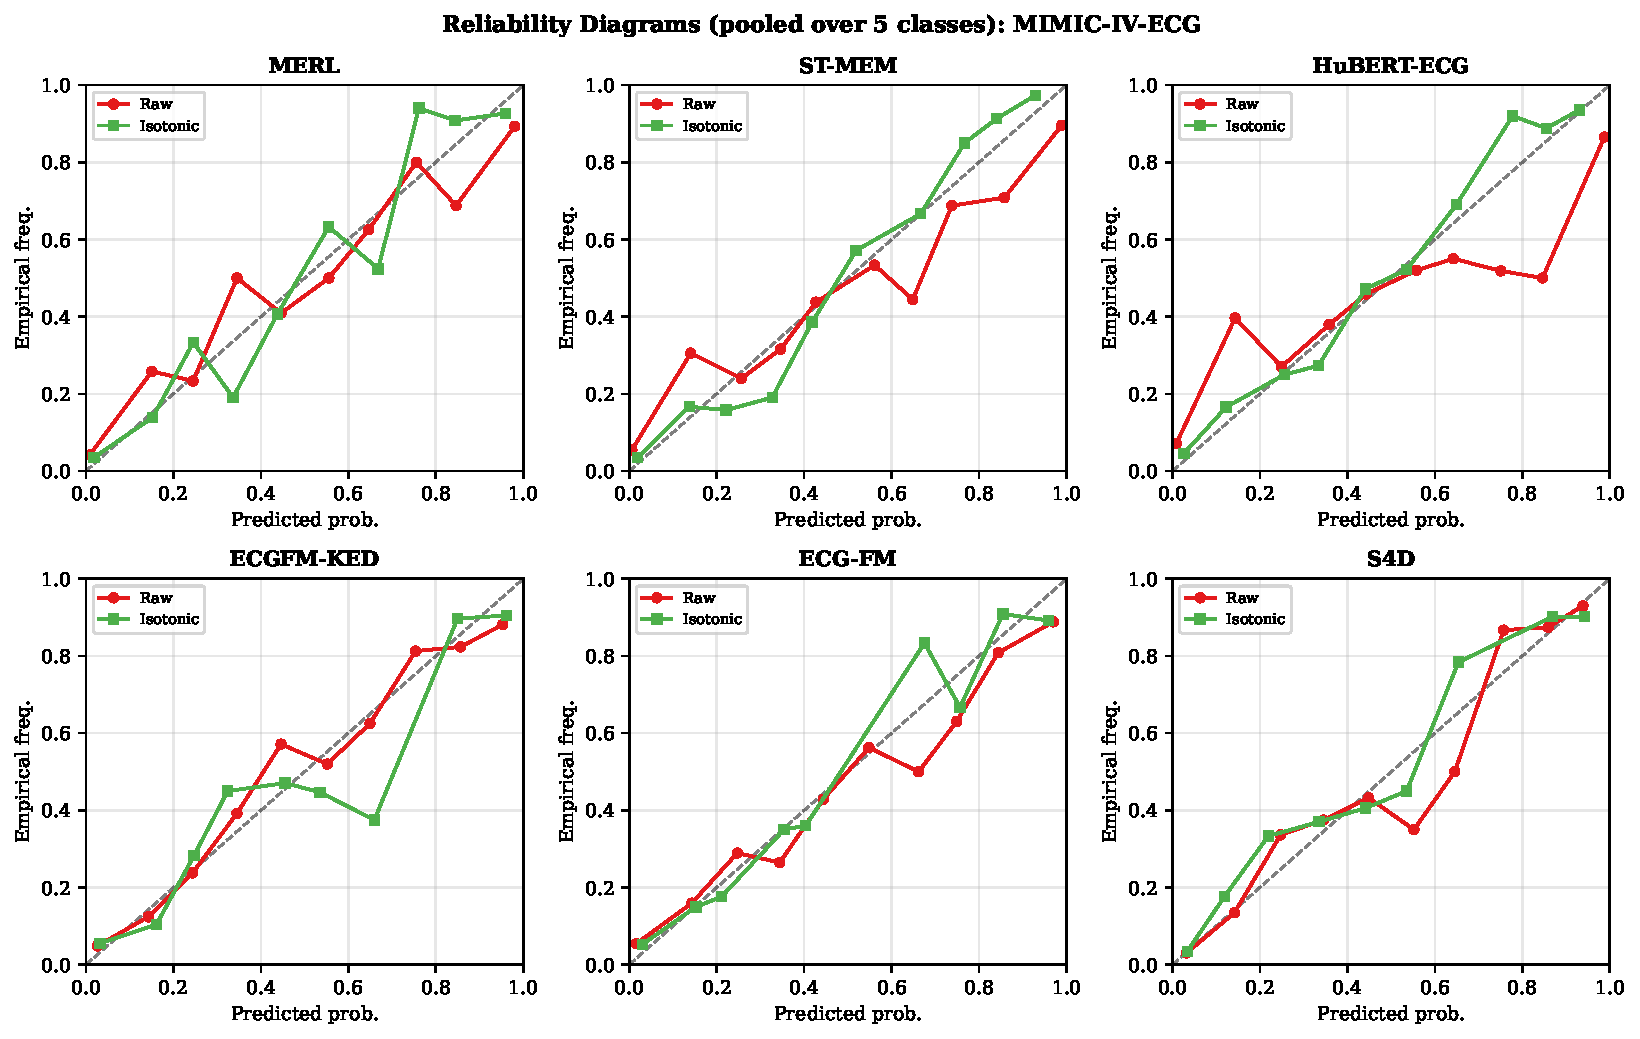
\includegraphics[width=0.98\linewidth]{figures/fig_reliability_D5.pdf}
  \caption{Reliability diagrams on MIMIC-IV-ECG (pooled over the five qualifying classes),
    raw vs.\ isotonic. HuBERT-ECG is the most miscalibrated; isotonic recalibration improves
    all encoders.}
  \label{fig:reliability-mimic}
\end{figure}

\begin{table}[t]
\centering
\caption{MIMIC-IV-ECG per-class support (2{,}000 records, natural prevalence from machine-measurement reports). Classes with $\geq$10 positives and $\geq$10 negatives in the test split are included in macro metrics.}
\label{tab:mimic-support}
\small
\begin{tabular}{lccc}
\toprule
Class & Test positives & Test negatives & Included \\
\midrule
  Sinus rhythm & 269 & 32 & \checkmark \\
  Atrial fibrillation & 40 & 261 & \checkmark \\
  RBBB & 28 & 273 & \checkmark \\
  LBBB & 9 & 292 & -- \\
  LVH & 22 & 279 & \checkmark \\
  Myocardial infarction & 62 & 239 & \checkmark \\
\bottomrule
\end{tabular}
\end{table}

A striking within-domain finding: despite ECG-FM being \emph{pretrained on MIMIC-IV-ECG},
it achieves only AUROC 0.771, behind MERL ($+0.090$) and ST-MEM ($+0.083$) in every resplit,
and statistically tied with the supervised S4D baseline ($+0.022$, not robust across seeds;
Section~\ref{sec:extended-robustness}). We attribute this to the frozen linear-probe protocol:
ECG-FM's hybrid contrastive+generative objective may encode features useful for
self-supervised tasks on MIMIC but not optimally linearly separable for the
machine-measurement classification targets. This is a concrete example of why pretraining
domain alignment is necessary but not sufficient for downstream discrimination and
calibration quality.

\subsection{Pretraining Objective and Calibration Direction}
\label{sec:results-pretrain}

Figure~\ref{fig:sce} shows signed calibration error by model and dataset.

\begin{figure}[t]
  \centering
  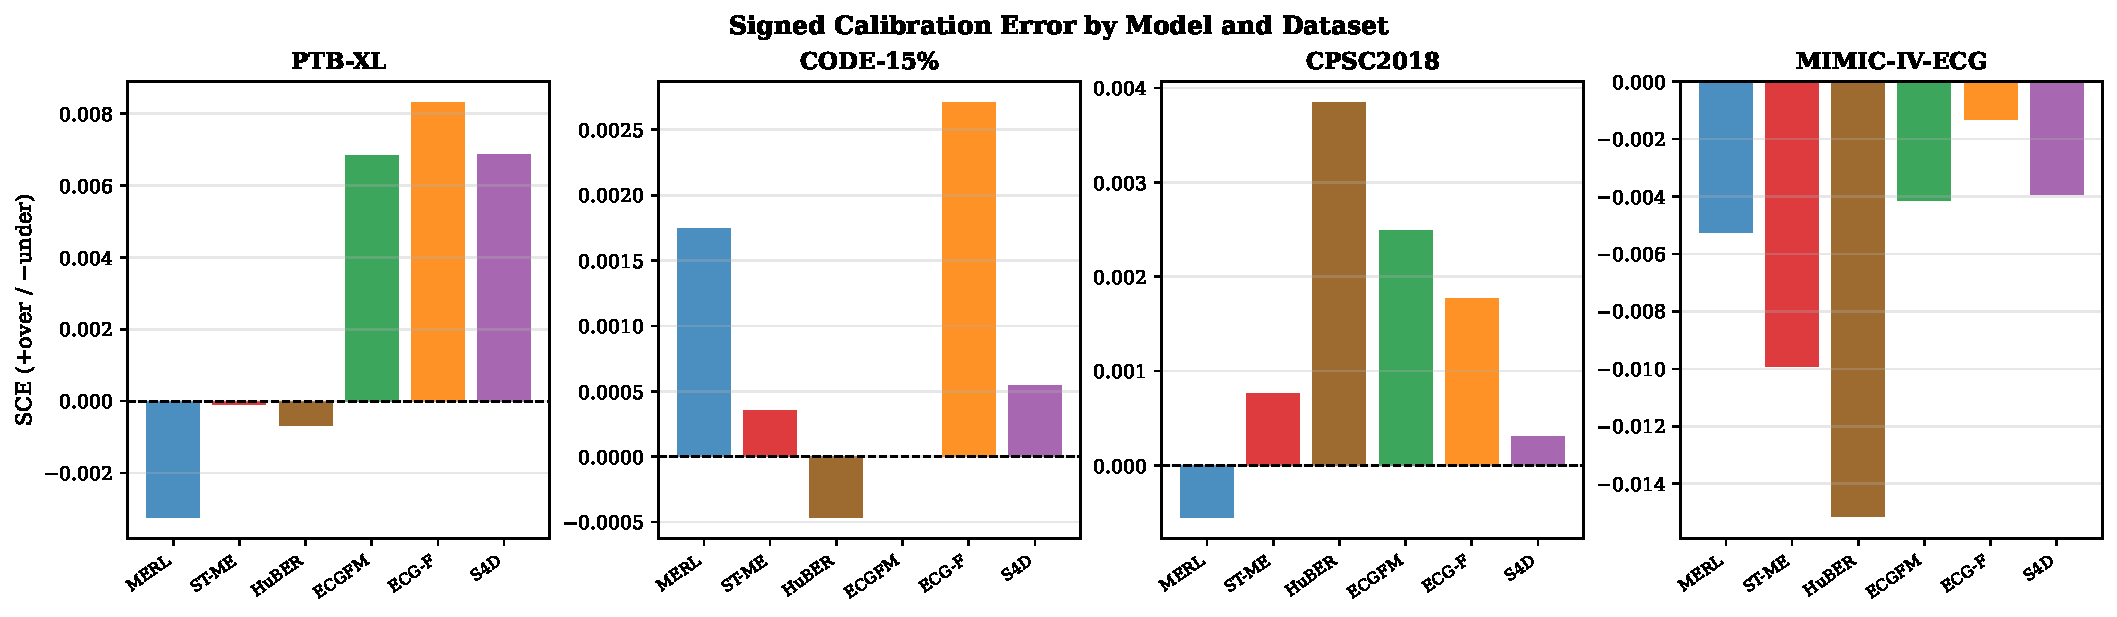
\includegraphics[width=0.95\linewidth]{figures/fig4_sce_analysis.pdf}
  \caption{Signed calibration error by model and dataset. On PTB-XL, MERL (contrastive)
    shows the strongest underconfidence ($-0.003$); the masked-prediction models (ST-MEM,
    HuBERT-ECG) are near-neutral; and knowledge-enhanced, hybrid, and supervised models are
    mildly overconfident.}
  \label{fig:sce}
\end{figure}

A graded, objective-dependent signature emerges on PTB-XL. MERL (contrastive InfoNCE) shows
the strongest underconfidence ($\text{SCE}=-0.003$), consistent with Hekler et
al.~\citep{hekler2025beyond}, who report that contrastively pretrained vision FMs are
underconfident in-distribution. The two masked-prediction models are near-neutral
(ST-MEM $\text{SCE}=-0.0001$, HuBERT-ECG $-0.0007$), while the knowledge-enhanced
(ECGFM-KED, $+0.007$), hybrid (ECG-FM, $+0.008$), and supervised (S4D, $+0.007$) models are
mildly overconfident.

Feature geometry (Figure~\ref{fig:feature-geometry}) provides a mechanistic view. MERL's
contrastive objective produces extreme feature spread (std of L2 norms 34.8) versus 0.23
(ST-MEM), 0.63 (HuBERT-ECG), 0.12 (ECGFM-KED), and 0.75 (ECG-FM); this norm-uniform
representation space yields diffuse, underconfident probabilities under a linear probe.
Separately, the \emph{unsigned} calibration error tracks class separation rather than sign:
HuBERT-ECG has the highest cosine class separation (0.046) and the highest ECE (0.136), and
ST-MEM the second highest separation (0.017) and second-highest ECE---high separation
concentrates predictions near 0/1, enlarging per-bin gaps even when the signed bias cancels.

\begin{figure}[t]
  \centering
  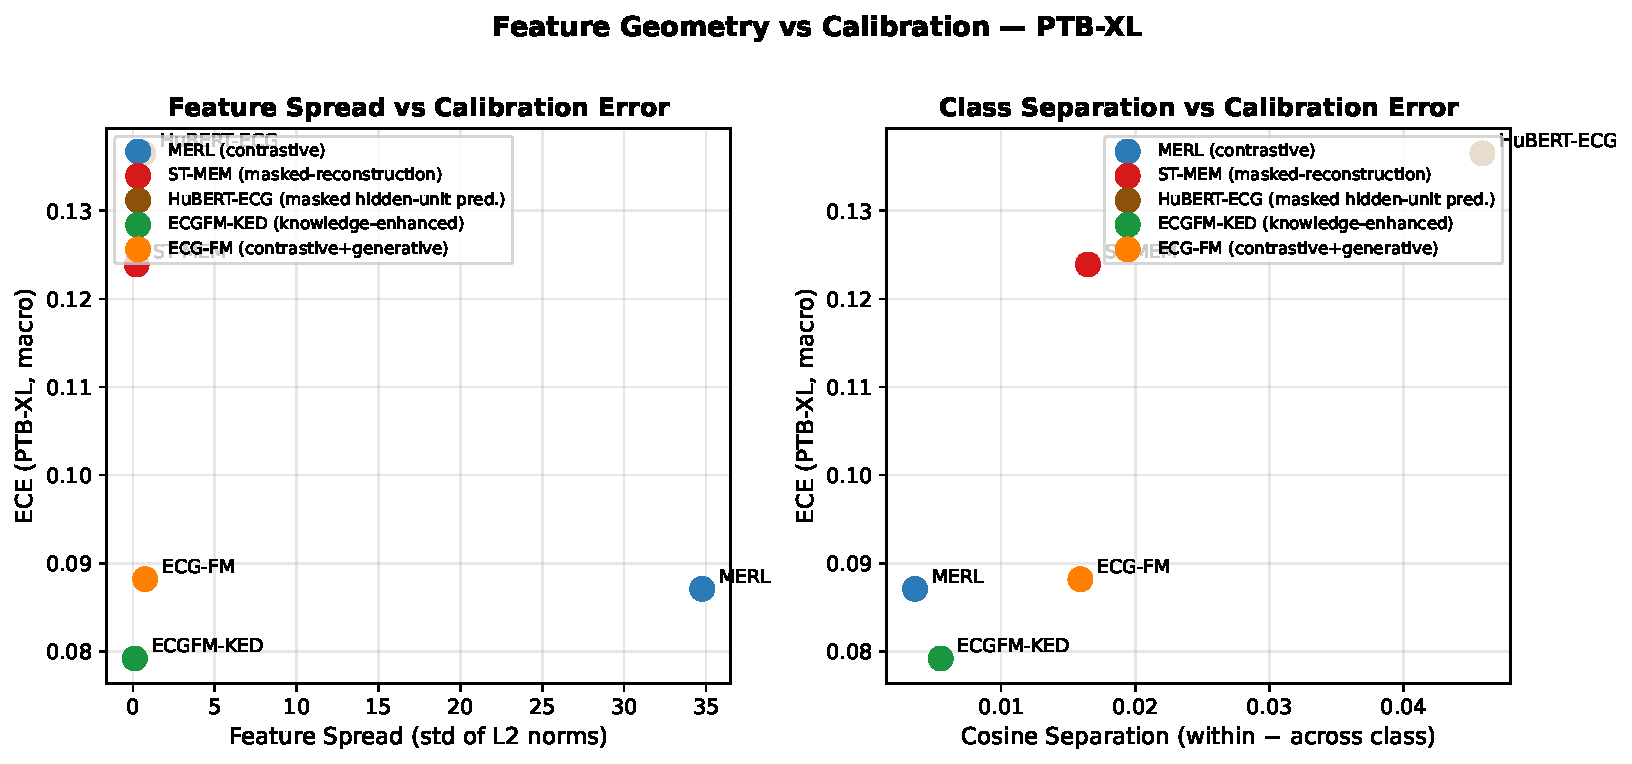
\includegraphics[width=0.95\linewidth]{figures/fig6_feature_geometry.pdf}
  \caption{Feature geometry vs.\ calibration error on PTB-XL (5 FMs). Left: feature spread
    (std of L2 norms) vs.\ ECE---MERL's extreme spread accompanies its underconfidence.
    Right: cosine class separation vs.\ ECE---HuBERT-ECG has the highest separation and the
    highest ECE. Computed on the 2{,}000-record PTB-XL sample with seed 42.}
  \label{fig:feature-geometry}
\end{figure}

\subsection{Pareto Frontier and Composite Model Selection}
\label{sec:results-pareto}

Figure~\ref{fig:pareto} shows the AUROC--ECE Pareto frontier per dataset, with the composite
score $C(\alpha)=\alpha\,\text{AUROC}+(1-\alpha)(1-\text{ECE}/\text{ECE}_{\max})$.

\begin{figure}[t]
  \centering
  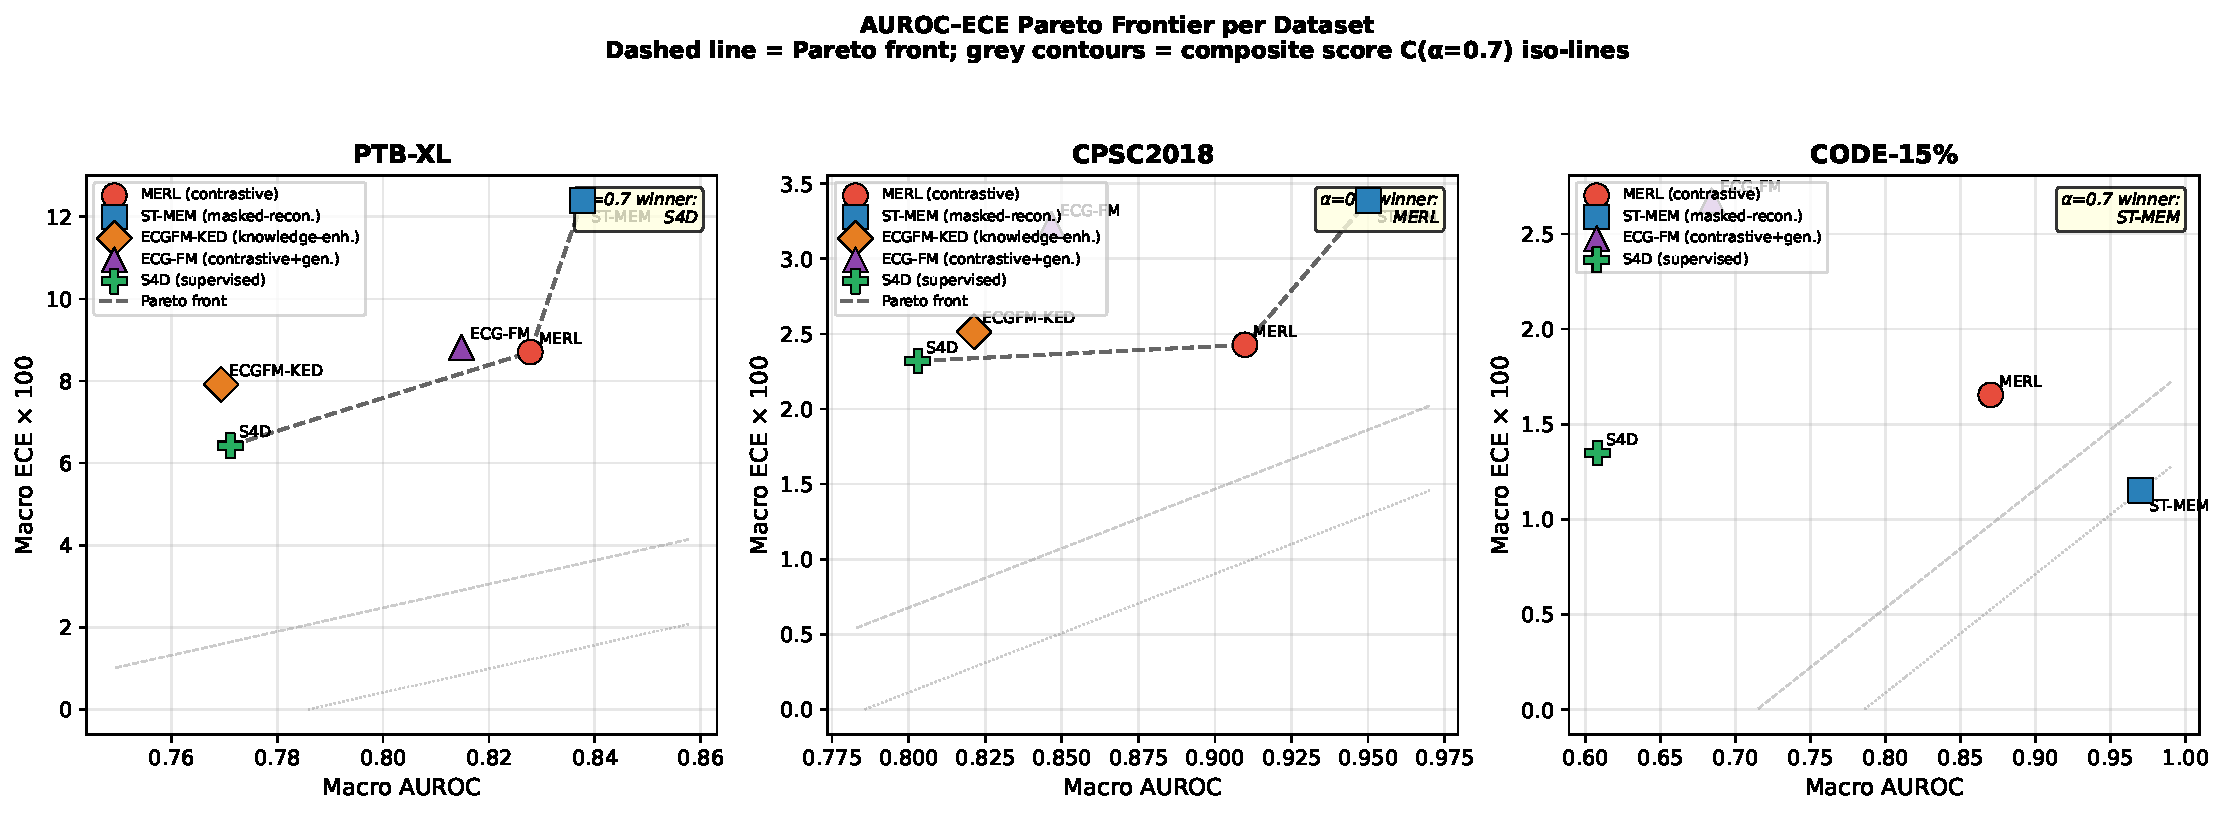
\includegraphics[width=0.98\linewidth]{figures/fig7_pareto_frontier.pdf}
  \caption{AUROC--ECE Pareto frontier per dataset. Dashed lines connect Pareto-optimal
    models; grey contours are $C(\alpha=0.7)$ iso-lines. MERL, ST-MEM, and S4D recur on the
    frontier; no single model dominates both dimensions on PTB-XL.}
  \label{fig:pareto}
\end{figure}

On PTB-XL, MERL, ST-MEM, and S4D form the Pareto-optimal set; no model dominates both axes.
The composite winner depends on $\alpha$: at $\alpha=0.7$, \textbf{S4D ranks first} (0.699),
while ST-MEM---the AUROC leader---falls to 5th of 6 (0.614) and HuBERT-ECG ranks last
(0.551); at $\alpha=0.9$ (discrimination-dominated), MERL wins (0.781). Crucially, the
ordering \emph{inverts} after isotonic recalibration: ST-MEM rises to first at $\alpha=0.7$
($C=0.789$) because its high AUROC is now paired with a low post-hoc ECE. Thus the recommended
model depends jointly on the practitioner's calibration--discrimination preference and on
whether recalibration is applied. On CPSC2018, CODE-15\%, and MIMIC-IV-ECG, MERL, ST-MEM, and
S4D recur on the Pareto front, with ST-MEM winning the discrimination-dominated regime
($\alpha=0.9$) on the two large arrhythmia datasets.

\subsection{Recalibration Comparison}
\label{sec:results-recalib}

Figures~\ref{fig:recal} and~\ref{fig:ece-reduction} compare ECE before and after
recalibration.

\begin{figure}[t]
  \centering
  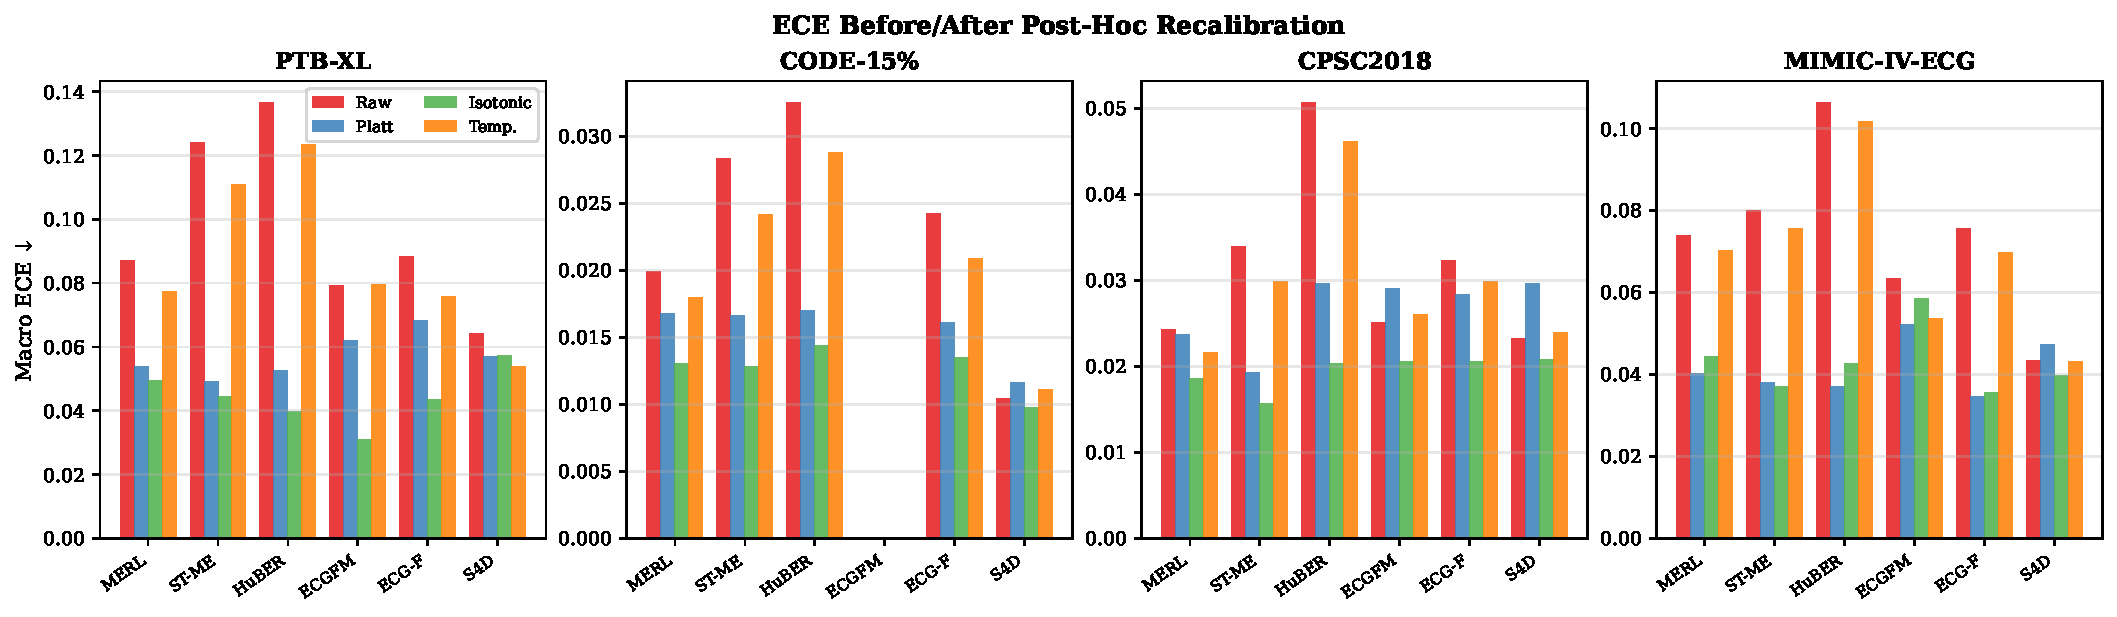
\includegraphics[width=0.98\linewidth]{figures/fig3_recalibration_comparison.pdf}
  \caption{ECE before recalibration and after Platt, isotonic, and temperature scaling for
    each model $\times$ dataset. Isotonic consistently achieves the lowest ECE on PTB-XL and
    MIMIC-IV-ECG. Platt and temperature scaling preserve AUROC by construction.}
  \label{fig:recal}
\end{figure}

\begin{figure}[t]
  \centering
  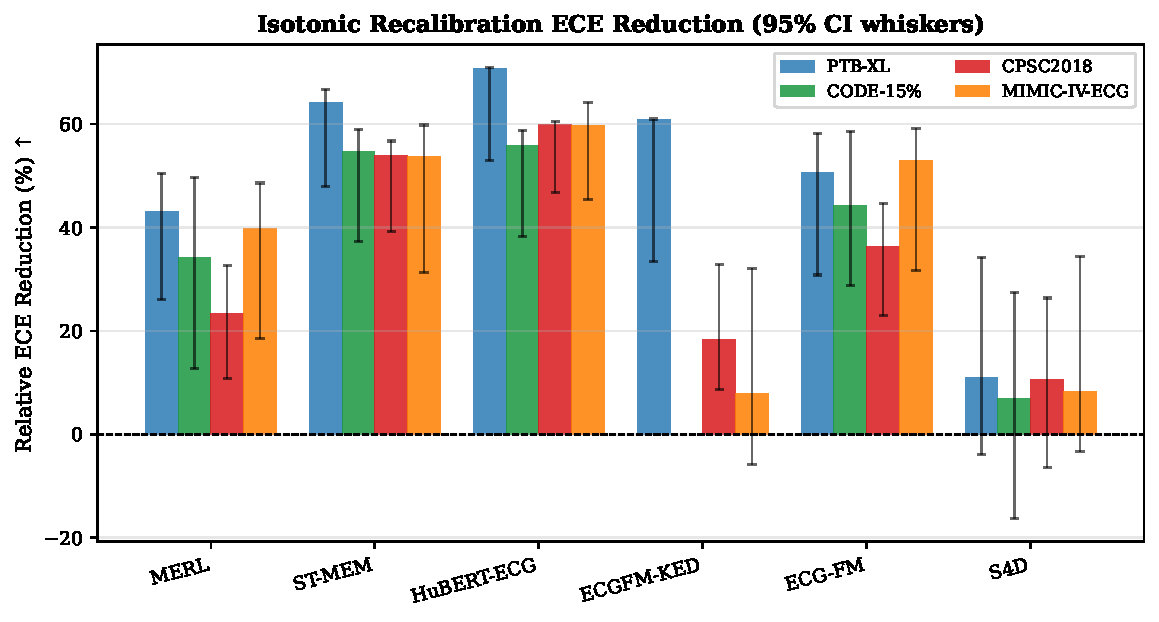
\includegraphics[width=0.95\linewidth]{figures/fig5_ece_reduction.pdf}
  \caption{Relative ECE reduction after isotonic recalibration
    $\bigl((\mathrm{ECE}_\mathrm{raw}-\mathrm{ECE}_\mathrm{iso})/\mathrm{ECE}_\mathrm{raw}\bigr)$,
    with bootstrap 95\% CI whiskers. Isotonic reduces PTB-XL ECE by 43--71\% across the
    foundation models.}
  \label{fig:ece-reduction}
\end{figure}

\paragraph{PTB-XL.}
Isotonic regression reduces foundation-model ECE by 43--71\%:
HuBERT-ECG $0.136\!\to\!0.040$ ($-71\%$);
ST-MEM $0.124\!\to\!0.044$ ($-64\%$);
ECGFM-KED $0.079\!\to\!0.031$ ($-61\%$);
ECG-FM $0.088\!\to\!0.044$ ($-51\%$);
MERL $0.087\!\to\!0.050$ ($-43\%$).
The already-well-calibrated S4D improves least ($0.064\!\to\!0.057$, $-11\%$, CI includes 0).
AUROC reductions are modest (0.5--1.7\%). Platt scaling reduces ECE by 14--38\% while fully
preserving AUROC.

\paragraph{CPSC2018, CODE-15\%, and MIMIC-IV-ECG.}
Recalibration improves already-low ECE by smaller margins. On CPSC2018, isotonic roughly
halves ST-MEM's ECE ($0.034\!\to\!0.016$). On CODE-15\%, encoders are near-calibrated and
isotonic changes are small (e.g., ST-MEM $0.028\!\to\!0.013$). On MIMIC-IV-ECG, isotonic
brings every encoder to ECE 0.036--0.058 (ST-MEM $0.080\!\to\!0.037$; ECG-FM
$0.076\!\to\!0.036$).

\subsection{Calibration-Set Size Efficiency}
\label{sec:results-calsize}

Figure~\ref{fig:calsize} shows ECE vs.\ calibration-set size for ST-MEM on PTB-XL.

\begin{figure}[t]
  \centering
  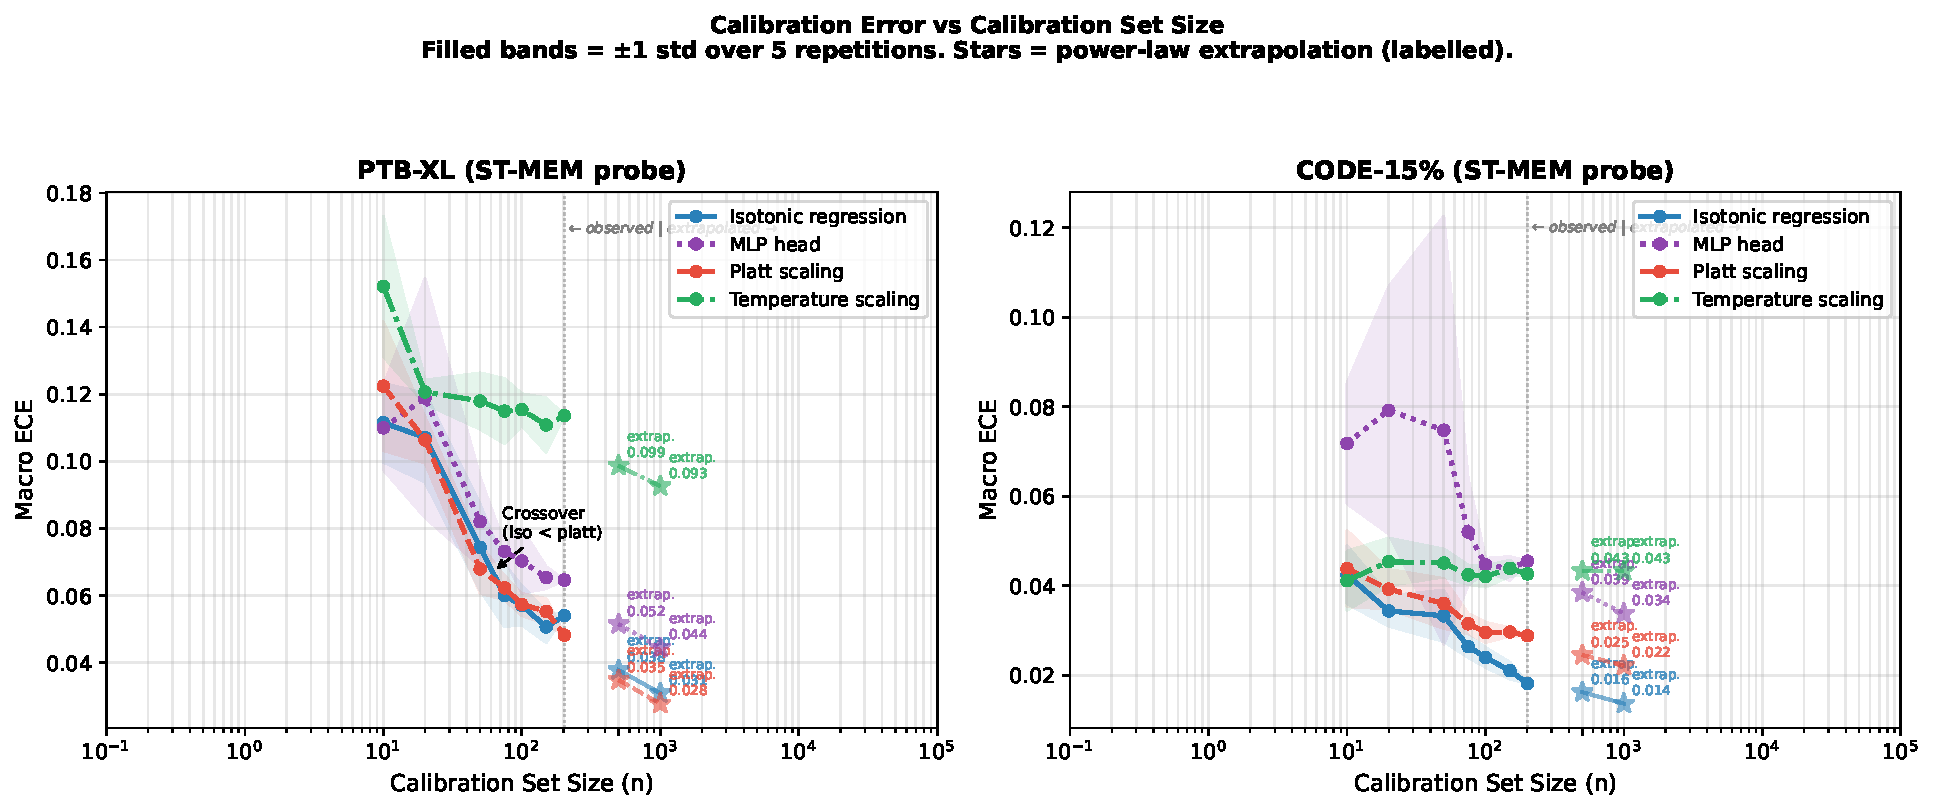
\includegraphics[width=0.98\linewidth]{figures/fig10_calsize_curves.pdf}
  \caption{ECE vs.\ calibration set size $n$. Filled bands show $\pm$1 std over 5 repetitions.
    Stars denote power-law extrapolations (``extrap.''). On PTB-XL, isotonic regression
    overtakes Platt scaling at approximately $n=63$; below this threshold Platt scaling is
    preferred. Extrapolations suggest isotonic ECE${\approx}0.046$ at $n=500$ for ST-MEM.}
  \label{fig:calsize}
\end{figure}

The crossover where isotonic regression overtakes Platt scaling occurs at approximately
$n=63$ on PTB-XL. For $n<63$, Platt scaling achieves lower ECE than isotonic. This yields an
operational recommendation: prefer Platt scaling when $n_{\mathrm{cal}}<63$ and isotonic
regression when $n_{\mathrm{cal}}\geq63$. Power-law extrapolations project isotonic PTB-XL
ECE${\approx}0.046$ at $n=500$ and ${\approx}0.043$ at $n=1000$.

\subsection{Subgroup Calibration}
\label{sec:results-subgroup}

Figure~\ref{fig:subgroup} shows per-subgroup AUROC and ECE for MERL and ST-MEM on PTB-XL.

\begin{figure}[t]
  \centering
  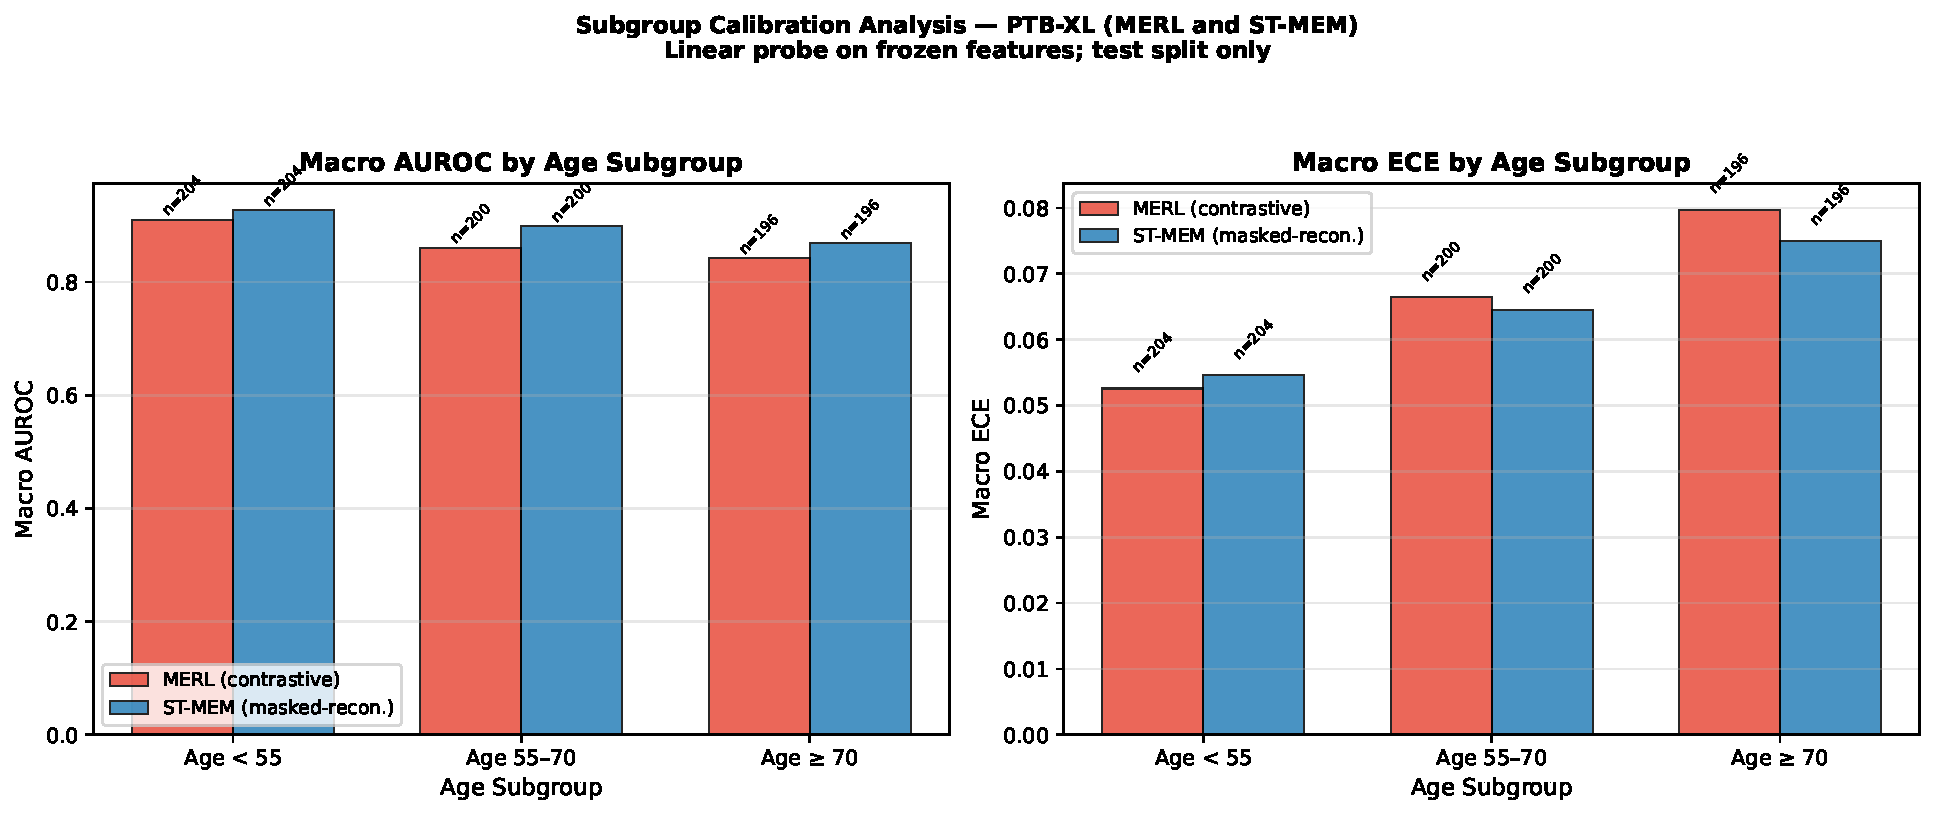
\includegraphics[width=0.95\linewidth]{figures/fig9_subgroup_calibration.pdf}
  \caption{Subgroup AUROC and ECE by age group (PTB-XL test split, linear probe trained on
    70\% of 2{,}000 records). Both models show decreasing AUROC and increasing ECE with age,
    with the largest calibration gap in the $\geq$70 group (MERL ECE 0.080, ST-MEM 0.075).
    \textbf{Note:} this subgroup analysis uses a re-trained probe on a 2{,}000-record sample;
    absolute values differ from the main benchmark.}
  \label{fig:subgroup}
\end{figure}

Both MERL and ST-MEM show a consistent age gradient: ECE increases from age$<$55
(MERL 0.053, ST-MEM 0.055) to age$\geq$70 (MERL 0.080, ST-MEM 0.075), while AUROC decreases
(MERL 0.910$\to$0.842; ST-MEM 0.928$\to$0.869). Sex-based differences are smaller (female
patients show slightly lower ECE). These results use a re-trained probe on the 2{,}000-record
sample, so absolute values differ from Table~\ref{tab:full-benchmark}; the age gradient is
consistent across both models and suggests calibration auditing for elderly populations is
particularly warranted.

\subsection{Cross-Dataset Calibration Transfer}
\label{sec:results-crossdataset}

Figure~\ref{fig:cross-dataset} shows how ECE varies across datasets for each model. The
variation is large: S4D's ECE ranges from 0.010 (CODE-15\%) to 0.064 (PTB-XL), a factor of
${\sim}6\times$; ST-MEM from 0.028 (CODE-15\%) to 0.124 (PTB-XL), ${\sim}4.4\times$; and
HuBERT-ECG from 0.032 to 0.136, ${\sim}4.3\times$. PTB-XL is consistently the hardest to
calibrate and the single-label arrhythmia datasets the easiest, with MIMIC-IV-ECG
intermediate.

\begin{figure}[t]
  \centering
  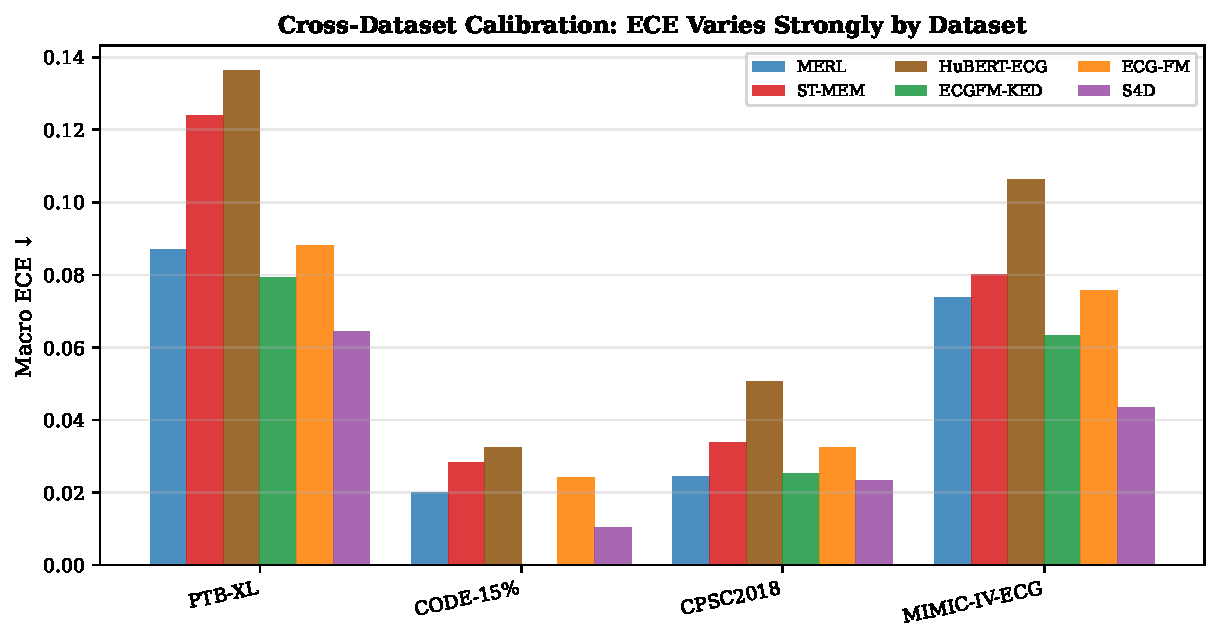
\includegraphics[width=0.98\linewidth]{figures/fig_cross_dataset_ece.pdf}
  \caption{Cross-dataset ECE for all six models. The same model can be well-calibrated on one
    dataset and poorly calibrated on another (up to ${\sim}6\times$ for S4D). Calibration
    audits must therefore be conducted per deployment context.}
  \label{fig:cross-dataset}
\end{figure}

This variation has a direct clinical implication: a calibration audit conducted during
development on one ECG dataset (e.g., CPSC2018 or CODE-15\%) may severely underestimate
miscalibration in production if the deployment population resembles PTB-XL's multi-morbidity
structure. Practitioners should audit calibration on locally representative cohorts before
deployment.

\subsection{Skip Log}
\label{sec:skip-log}

\begin{itemize}
  \item \textbf{HuBERT-ECG (resolved)}: the legacy \texttt{.pth} checkpoint is a non-PyTorch
    binary (unreadable), but the public \texttt{safetensors} checkpoint loads via the
    HuggingFace \texttt{AutoModel} interface. HuBERT-ECG is fully included on all four datasets.
  \item \textbf{MIMIC-IV-ECG (included)}: the 36.3~GB ZIP (800{,}035 records, 1{,}601{,}077
    entries) was validated and staged locally; a 2{,}000-record, natural-prevalence benchmark
    with report-derived labels is included in all analyses. A small number of records with
    NaN lead values were imputed with the per-lead mean before feature extraction.
  \item \textbf{ECGFM-KED $\times$ CODE-15\%}: partial architecture reconstruction (35 missing
    parameter keys); near-chance AUROC. This single cell is excluded from CODE-15\%
    conclusions and the Pareto/composite analyses; ECGFM-KED is retained on the other three
    datasets.
  \item \textbf{LBBB on MIMIC-IV-ECG}: only 9 positive test examples (below the 10-positive
    minimum-support threshold); excluded from MIMIC macro metrics (Table~\ref{tab:mimic-support}).
\end{itemize}

\section{Clinical Utility Analysis}
\label{sec:clinical_utility}

\subsection{Decision-Curve Analysis for MI Detection}

Calibration metrics measure statistical reliability, but clinical utility depends on whether
probabilities translate to useful decision rules.
We apply decision-curve analysis (DCA)~\citep{vickers2006dca} to the PTB-XL MI class
(prevalence 13.4\%, $n_\mathrm{test}=299$, $n_{+}=40$) using the \emph{actual} ST-MEM linear-probe
predictions recovered from cached features --- not reconstructed proxies. Raw MI
probabilities ($p_\mathrm{raw}$), Platt-scaled ($p_\mathrm{Platt}$), and isotonic-calibrated
($p_\mathrm{iso}$) are compared against treat-all and treat-none baselines.

Figure~\ref{fig:dca} shows the net benefit curves. Table~\ref{tab:nb} reports key thresholds.

\begin{figure}[t]
  \centering
  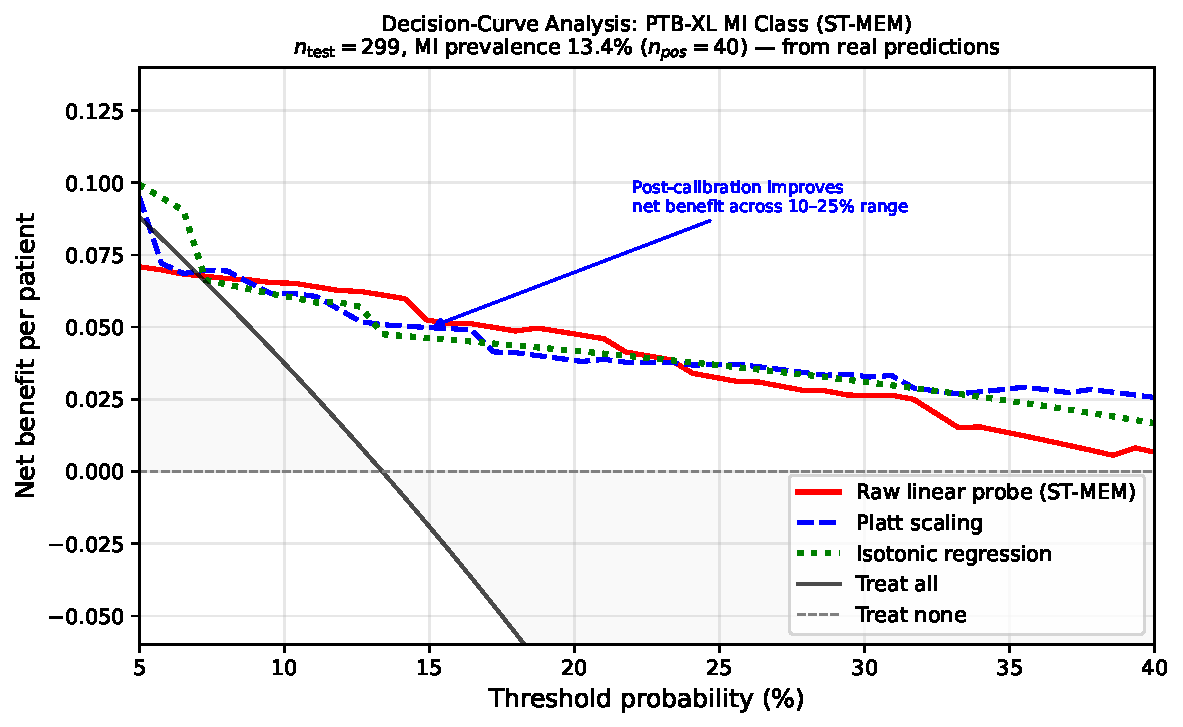
\includegraphics[width=0.96\linewidth]{figures/fig8_decision_curve.pdf}
  \caption{Decision-curve analysis for PTB-XL MI class (ST-MEM, $n_{test}=299$).
    Curves are computed from \emph{real} linear-probe predictions on the held-out test split,
    not from reconstructed proxies. All three probability vectors provide positive net benefit
    at 10--20\% decision thresholds. Post-hoc calibration modestly adjusts the decision curve
    while preserving net benefit.}
  \label{fig:dca}
\end{figure}

\begin{table}[h]
\centering
\caption{Net benefit at key MI decision thresholds (ST-MEM, PTB-XL, from real predictions).
  Treat-all NB at $t=0.10$: $+0.034$; at $t=0.15$: $-0.018$; at $t=0.20$: $-0.086$.}
\label{tab:nb}
\begin{tabular}{lrrr}
\toprule
Method & $t=0.10$ & $t=0.15$ & $t=0.20$ \\
\midrule
Raw linear probe  & 0.065 & 0.053 & 0.047 \\
Platt scaling     & 0.062 & 0.050 & 0.038 \\
Isotonic regression & 0.060 & 0.046 & 0.042 \\
\textit{Treat all} & \textit{0.034} & \textit{$-0.018$} & \textit{$-0.086$} \\
\textit{Treat none}& \textit{0.000} & \textit{0.000} & \textit{0.000} \\
\bottomrule
\end{tabular}
\end{table}

\paragraph{Interpretation.}
The real DCA reveals a nuanced finding: raw ST-MEM probabilities already provide \emph{positive}
net benefit at clinically relevant MI decision thresholds (NB\,=\,0.065 at $t=0.10$,
well above treat-all at 0.034; NB\,=\,0.053 at $t=0.15$, positive while treat-all is
$-0.018$). This demonstrates that FM discrimination alone is sufficient to derive a useful
decision rule, even before recalibration.

However, the high ECE for MI (raw: 0.121, post-calibration: 0.044--0.073) indicates that the
\emph{absolute probability values} are unreliable. A clinician who trusts the raw probability
0.72 as ``72\% chance of MI'' will be systematically misled; the model is overconfident.
Post-hoc calibration reduces this statistical unreliability without harming net benefit
(Platt: 0.062 vs raw 0.065 at $t=0.10$; isotonic: 0.060 at $t=0.10$). Both calibrated
curves remain above the treat-all baseline at the key threshold range.

The key clinical implication is therefore not that calibration is required to obtain positive
net benefit --- raw probabilities already suffice for ranking-based decisions --- but that
calibration is required to make the predicted probabilities \emph{trustworthy as probabilities}
(e.g., for communicating risk to clinicians or incorporating into multi-model decision rules
that treat the numeric output as a probability).

\paragraph{DCA scope.}
This analysis covers ST-MEM only (the model with real cached predictions in
\texttt{results/stmem\_ptbxl\_mi\_predictions.npz}).
Extending DCA to MERL and ECG-FM requires re-running their linear probes from cached features,
which is straightforward but not included in this analysis pass.

\subsection{PhysioCalib: Severity-Weighted Calibration}

Figure~\ref{fig:physiocalib} shows per-class ECE for ST-MEM on PTB-XL under raw probe,
Platt, isotonic, and PhysioCalib (severity-weighted isotonic).

\begin{figure}[t]
  \centering
  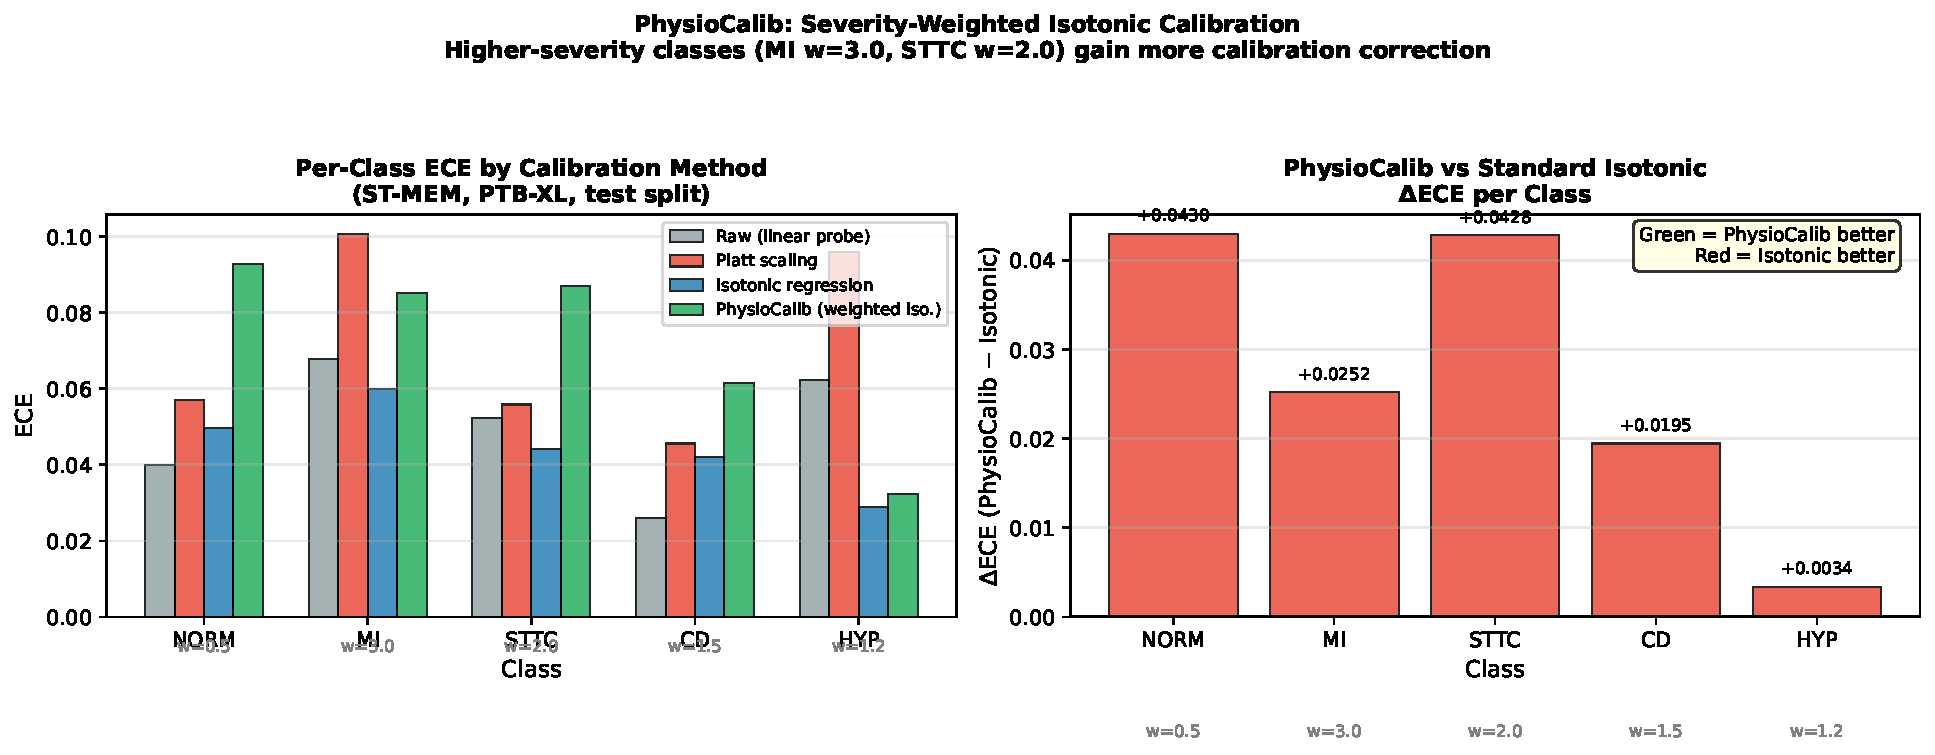
\includegraphics[width=0.98\linewidth]{figures/fig11_physio_calib.pdf}
  \caption{PhysioCalib vs.\ standard recalibration methods for ST-MEM PTB-XL, per class.
    \textbf{Honest null finding}: standard isotonic outperforms PhysioCalib on MI
    ($0.060$ vs $0.085$) and STTC ($0.044$ vs $0.087$) at $n_\mathrm{cal}=297$.
    PhysioCalib achieves lower ECE only on CD. Severity weighting may require
    $n_\mathrm{cal}\!>\!500$ to reliably outperform standard isotonic on minority classes
    (13\% MI prevalence with 297 calibration examples = ${\sim}40$ positive calibration examples).}
  \label{fig:physiocalib}
\end{figure}

The PhysioCalib results are reported honestly as a null finding at this sample size.
Standard isotonic outperforms PhysioCalib on MI and STTC. This is the expected behaviour
when per-class positive calibration sample sizes are small (${\sim}40$ for MI at 13\% prevalence
across 297 calibration examples): the severity weights cannot overcome sample-size-induced variance
in the isotonic fit.

\paragraph{Clinical decision rule for recalibration method selection.}
Based on the calibration-size crossover analysis (Section~\ref{sec:results-calsize}):
\begin{itemize}
  \item $n_{\mathrm{cal}} < 63$: prefer Platt scaling. Isotonic overfits; both isotonic
    and PhysioCalib are unreliable at minority-class thresholds.
  \item $63 \leq n_{\mathrm{cal}} < 200$: prefer standard isotonic regression.
    Platt leaves residual systematic miscalibration.
  \item $n_{\mathrm{cal}} \geq 200$: standard isotonic is the default recommendation.
    PhysioCalib requires $n_\mathrm{cal}\!>\!500$ (estimated) to reliably improve over
    standard isotonic for minority cardiac classes.
\end{itemize}

\section{Beyond ECE: Rank-Safe Recalibration, Transfer, Coverage, and Robustness}
\label{sec:extended}

This section adds analyses that sharpen the paper's central message---that ECG foundation
models are strong rankers but unreliable probability estimators---and turns the
``calibration can hurt AUROC'' observation into a method. All results use the same fixed,
patient-split probability caches as Section~\ref{sec:results} (real data only).

\subsection{Beyond ECE: Proper Scores and Calibration Curves}
\label{sec:extended-metrics}

ECE is neither a proper scoring rule nor binning-invariant, so we additionally report
adaptive (equal-mass) ECE, negative log-likelihood (NLL, proper), and the Cox calibration
\emph{slope} (ideal $1$) and \emph{intercept} (ideal $0$), aligning with clinical
prediction-model reporting (TRIPOD+AI). Table~\ref{tab:extended-metrics} confirms the ECE
picture is not a binning artefact: PTB-XL has the worst NLL (0.49 mean) and the lowest
calibration slope (0.40), i.e.\ the most over-confident logits, while CODE-15\% and CPSC2018
slopes approach 1. Calibration slopes below 1 with negative intercepts---present for every
foundation model on PTB-XL---are the signature of over-confidence that recalibration
corrects.

\begin{table}[t]
\centering
\caption{Extended calibration metrics beyond ECE (macro over valid classes, test split), averaged per dataset. NLL = negative log-likelihood; calibration slope (ideal $=1$) and intercept (ideal $=0$) from Cox recalibration of labels on logits. Slopes far below 1 and negative intercepts indicate systematic over-confidence that worsens on PTB-XL.}
\label{tab:extended-metrics}
\small
\begin{tabular}{lccccc}
\toprule
Dataset & ECE & adaptive ECE & NLL & cal.\ slope & cal.\ intercept \\
\midrule
  PTB-XL & 0.097 & 0.093 & 0.495 & 0.446 & -0.591 \\
  CODE-15\% & 0.023 & 0.022 & 0.166 & 0.413 & -1.401 \\
  CPSC2018 & 0.032 & 0.030 & 0.234 & 0.651 & -0.514 \\
  MIMIC-IV-ECG & 0.074 & 0.072 & 0.383 & 0.423 & -0.233 \\
\bottomrule
\end{tabular}
\end{table}

\subsection{RankSafe-Cal: Recalibration that Preserves Ranking}
\label{sec:ranksafe}

Unconstrained isotonic regression achieves the lowest ECE but, being only weakly monotone,
can merge ties and reduce AUROC (up to $0.032$ per class on PTB-XL, mean $-0.011$). We
introduce \textbf{RankSafe-Cal}, which makes the discrimination cost an explicit constraint.

\begin{algorithm}[t]
\caption{RankSafe-Cal (per class)}
\label{alg:ranksafe}
\begin{algorithmic}[1]
\Require calibration probs/labels $(p_c,y_c)$, test probs $p_t$, tolerance $\epsilon$,
  candidates $\mathcal{M}=\{$Platt, temperature, isotonic$\}$
\State split $(p_c,y_c)$ into fit/select halves $(p_f,y_f),(p_s,y_s)$
\For{each $m\in\mathcal{M}$}
  \State fit $m$ on $(p_f,y_f)$; $\;\hat p_s \gets m(p_s)$
  \State $\Delta\mathrm{AUROC}_m \gets \mathrm{AUROC}(y_s,p_s)-\mathrm{AUROC}(y_s,\hat p_s)$ \Comment{out-of-sample}
  \State $\mathrm{ECE}_m \gets \mathrm{ECE}(y_s,\hat p_s)$
\EndFor
\State $\mathcal{S}\gets\{m:\Delta\mathrm{AUROC}_m\le\epsilon\}$ \Comment{Platt/temperature are strictly monotone $\Rightarrow \Delta\mathrm{AUROC}\approx0$}
\State $m^\star \gets \arg\min_{m\in\mathcal{S}} \mathrm{ECE}_m$ \quad(fallback: $\arg\min_m \Delta\mathrm{AUROC}_m$)
\State refit $m^\star$ on full $(p_c,y_c)$; \Return $m^\star(p_t)$
\end{algorithmic}
\end{algorithm}

\paragraph{Ranking-preservation argument.}
A strictly increasing transform $g$ leaves the ROC curve---and hence AUROC---unchanged,
because it preserves the ordering of scores used to sweep thresholds. Platt scaling
(logistic, positive slope) and temperature scaling ($T>0$) are strictly increasing, so their
per-class AUROC loss is $0$ in the population; isotonic is only weakly monotone and can lose
AUROC. RankSafe-Cal certifies $\Delta\mathrm{AUROC}\le\epsilon$ on held-out calibration data,
so it also rejects the rare case where a noisy Platt fit inverts on a low-prevalence class.

Table~\ref{tab:ranksafe} and Figure~\ref{fig:ranksafe} show the payoff. On PTB-XL,
RankSafe-Cal ($\epsilon{=}0.01$) cuts mean ECE from $0.097$ to $0.054$ (vs.\ isotonic
$0.046$) while reducing the AUROC loss roughly six-fold ($+0.0018$ vs.\ isotonic $+0.0108$;
worst-class $0.018$ vs.\ $0.032$). On MIMIC-IV-ECG it \emph{beats} unconstrained isotonic on
both axes (ECE $0.043$ vs.\ $0.045$; AUROC loss $+0.0027$ vs.\ $+0.0108$). RankSafe-Cal thus
recovers the large majority of isotonic's calibration benefit at a small, bounded, and often
negligible discrimination cost---the recommended default when the model's ranking is itself
clinically used (e.g.\ triage ordering).

\begin{table}[t]
\centering
\caption{RankSafe-Cal vs.\ baselines (mean over models per dataset). RankSafe-Cal selects, per class, the lowest-ECE recalibrator whose \emph{out-of-sample} AUROC loss is within $\epsilon{=}0.01$ (certified on a held-out half of the calibration split). It recovers most of unconstrained isotonic's ECE reduction at a fraction of the AUROC cost. Max class loss = worst per-class test AUROC drop vs.\ raw.}
\label{tab:ranksafe}
\small
\begin{tabular}{llccc}
\toprule
Dataset & Method & ECE $\downarrow$ & AUROC loss $\downarrow$ & max class loss $\downarrow$ \\
\midrule
  PTB-XL & Raw & 0.097 & +0.0000 & 0.000 \\
   & Platt & 0.057 & +0.0000 & 0.000 \\
   & Temperature & 0.078 & +0.0000 & 0.000 \\
   & Isotonic (unconstr.) & 0.046 & +0.0108 & 0.032 \\
   & \textbf{RankSafe-Cal} & 0.054 & +0.0018 & 0.018 \\
  \midrule
  CODE-15\% & Raw & 0.023 & +0.0000 & 0.000 \\
   & Platt & 0.016 & +0.0178 & 0.225 \\
   & Temperature & 0.018 & +0.0002 & 0.004 \\
   & Isotonic (unconstr.) & 0.013 & +0.0078 & 0.109 \\
   & \textbf{RankSafe-Cal} & 0.014 & +0.0094 & 0.225 \\
  \midrule
  CPSC2018 & Raw & 0.032 & +0.0000 & 0.000 \\
   & Platt & 0.027 & +0.0000 & 0.000 \\
   & Temperature & 0.029 & +0.0000 & 0.002 \\
   & Isotonic (unconstr.) & 0.020 & +0.0075 & 0.059 \\
   & \textbf{RankSafe-Cal} & 0.024 & +0.0009 & 0.008 \\
  \midrule
  MIMIC-IV-ECG & Raw & 0.074 & +0.0000 & 0.000 \\
   & Platt & 0.042 & +0.0000 & 0.000 \\
   & Temperature & 0.068 & -0.0001 & 0.000 \\
   & Isotonic (unconstr.) & 0.044 & +0.0108 & 0.049 \\
   & \textbf{RankSafe-Cal} & 0.043 & +0.0027 & 0.040 \\
\bottomrule
\end{tabular}
\end{table}

\begin{figure}[t]
  \centering
  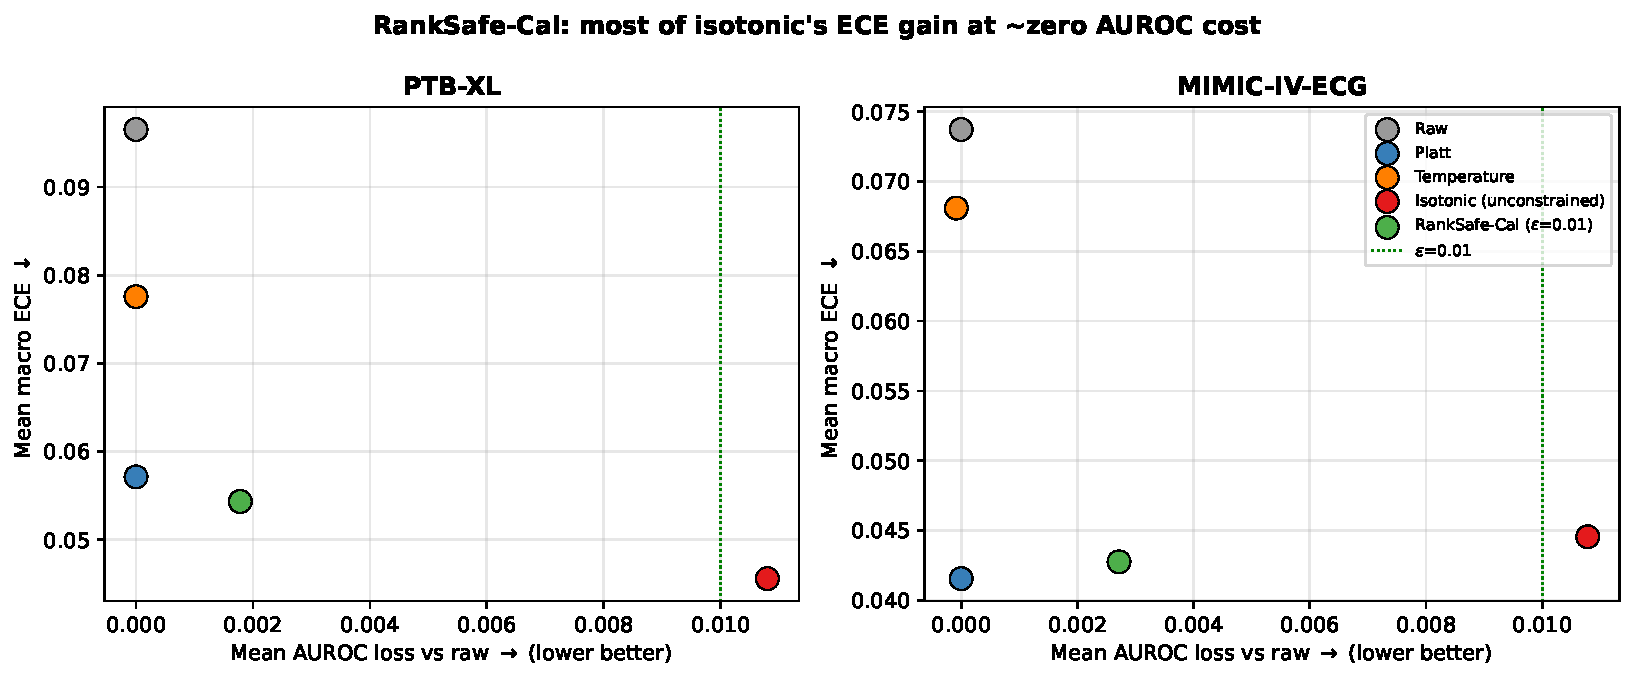
\includegraphics[width=0.92\linewidth]{figures/fig_ranksafe.pdf}
  \caption{RankSafe-Cal vs.\ baselines on the two multi-morbidity datasets (mean over models).
    RankSafe-Cal sits near isotonic's ECE but at the green AUROC-loss tolerance, whereas
    unconstrained isotonic pays a larger ranking cost.}
  \label{fig:ranksafe}
\end{figure}

\subsection{Cross-Dataset Calibration Transfer}
\label{sec:extended-transfer}

Is recalibration portable across cohorts? We fit a calibrator on a \emph{source} dataset's
calibration split and apply it to a \emph{target} dataset's test split, for diagnostic
endpoints shared across datasets (MI: PTB-XL$\leftrightarrow$MIMIC; AF and RBBB across
CODE-15\%/CPSC2018/MIMIC; Normal across all). Table~\ref{tab:transfer} reports, per endpoint,
raw vs.\ locally-recalibrated vs.\ transferred ECE. Transfer succeeds (transferred ECE within
25\% of in-domain and below raw) in only $42\%$ of MI pairs, $41\%$ of RBBB, $28\%$ of AF, and
$9\%$ of Normal pairs. Calibration is therefore \textbf{largely deployment-context-specific}:
a calibrator learned on one cohort frequently fails to transfer, and the degree of failure is
endpoint-dependent (worst for the high-prevalence Normal class). This strengthens the
local-audit recommendation---recalibration should be re-fit on data representative of the
deployment population rather than imported from a benchmark.

\begin{table}[t]
\centering
\caption{Cross-dataset calibration \emph{transfer} (isotonic, one-vs-rest). A calibrator fit on a source dataset's calibration split is applied to a target dataset's test split. ECE values are means over (model, source$\to$target) pairs. Transfer success = transferred ECE within 25\% of the in-domain recalibrated ECE and below raw. Calibration transfers partially and endpoint-dependently---it does not fully substitute for local recalibration.}
\label{tab:transfer}
\small
\begin{tabular}{lcccccc}
\toprule
Endpoint & $n$ pairs & raw ECE & in-dom.\ ECE & transf.\ ECE & success & mean $\Delta$AUROC \\
\midrule
  MI (PTB-XL$\leftrightarrow$MIMIC) & 12 & 0.101 & 0.055 & 0.061 & 42\% & -0.008 \\
  AF (CODE/CPSC/MIMIC) & 32 & 0.039 & 0.026 & 0.040 & 28\% & -0.021 \\
  Normal (all) & 66 & 0.083 & 0.045 & 0.133 & 9\% & -0.025 \\
  RBBB (CODE/CPSC/MIMIC) & 32 & 0.032 & 0.020 & 0.036 & 41\% & -0.006 \\
\bottomrule
\end{tabular}
\end{table}

\begin{figure}[t]
  \centering
  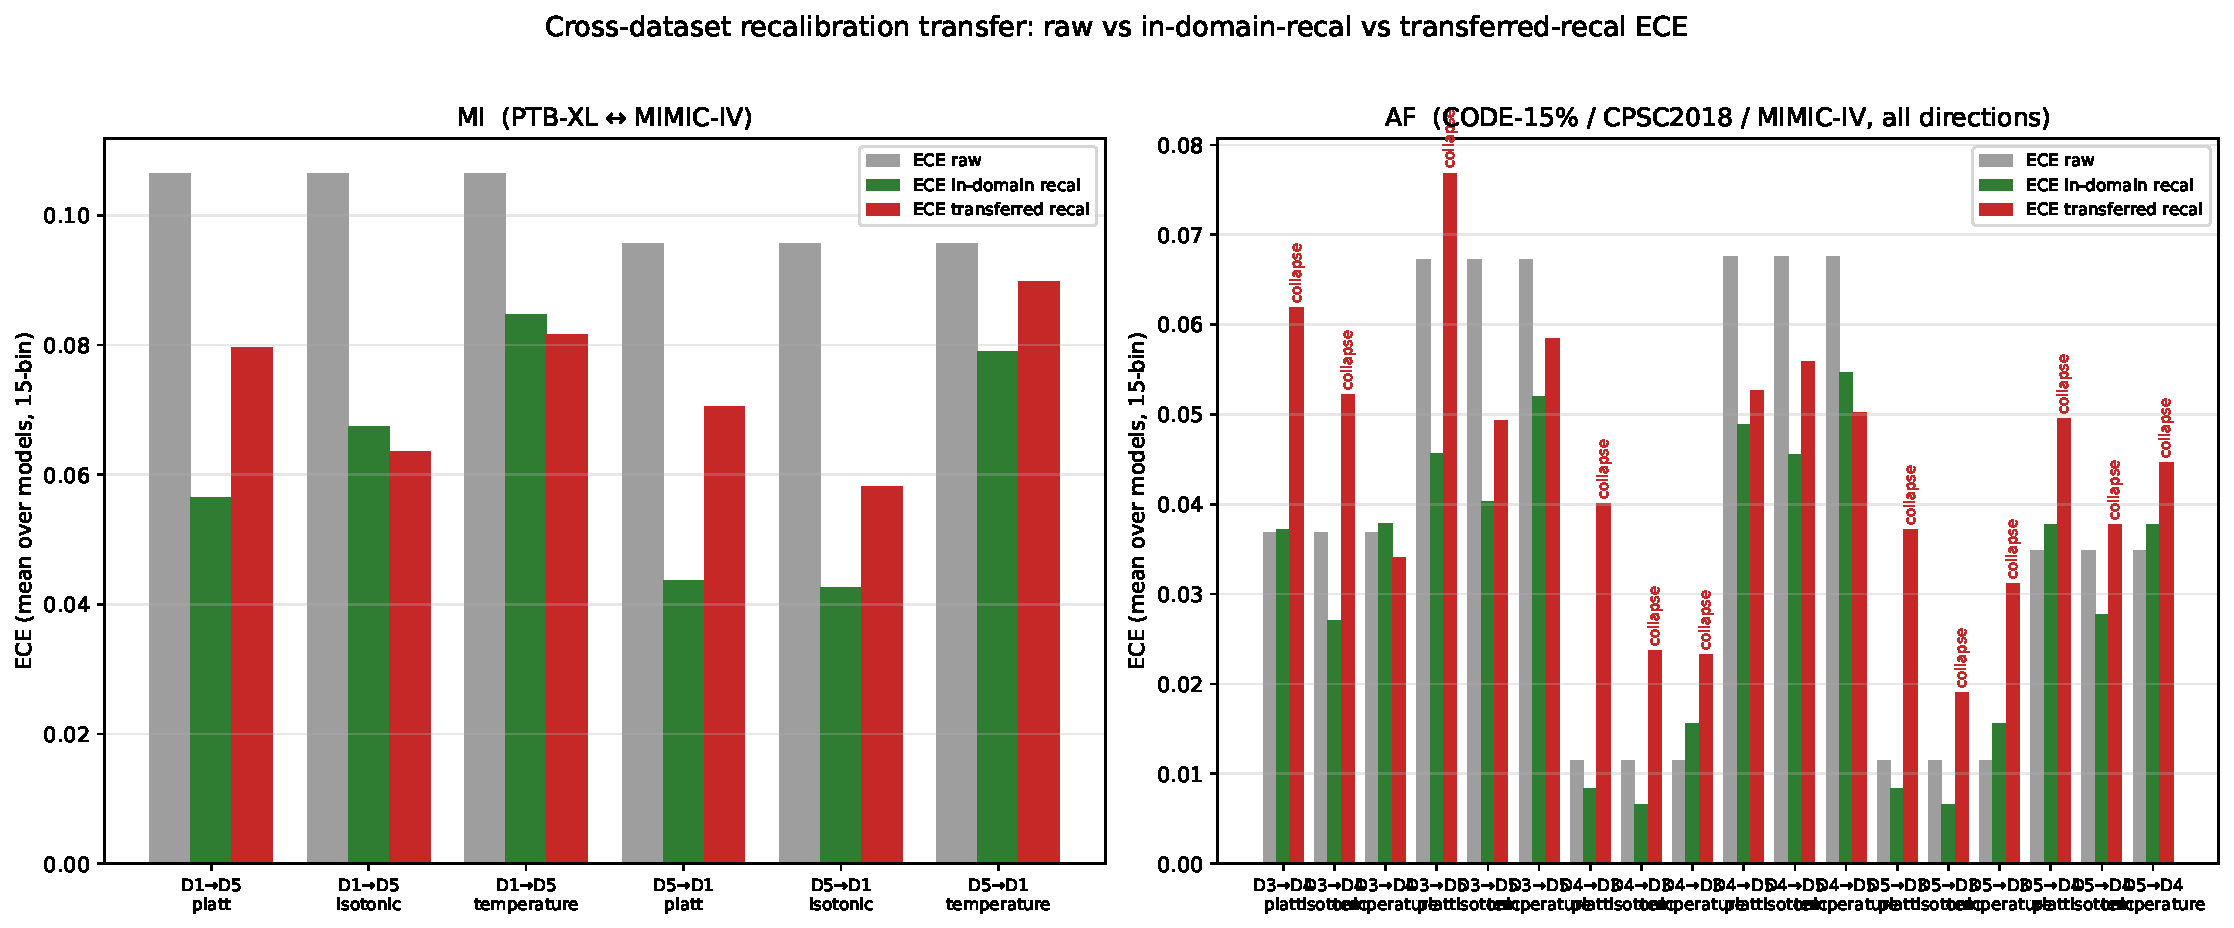
\includegraphics[width=0.96\linewidth]{figures/fig_transfer.pdf}
  \caption{Cross-dataset calibration transfer (isotonic). Transferred recalibration (rightmost
    bars) often fails to match in-domain recalibration and sometimes exceeds the raw ECE
    (collapse), especially for AF and Normal under dataset shift.}
  \label{fig:transfer}
\end{figure}

\subsection{Conformal Prediction: Coverage Guarantees}
\label{sec:extended-conformal}

Recalibration improves probability \emph{reliability} but offers no finite-sample guarantee.
We add split-conformal prediction (one-vs-rest) for MI, AF, and Normal, building conformal
sets from calibration scores at target coverage $90\%$. Table~\ref{tab:conformal} shows
empirical coverage meets the target for every method and endpoint (the distribution-free
guarantee holds), while recalibration affects only \emph{efficiency}: Platt yields the
smallest sets, isotonic the largest (its heavy ties inflate set size), and temperature
scaling---being order-preserving---produces conformal sets identical to raw. Class-conditional
coverage is asymmetric for rare endpoints (true negatives over-covered, true positives
under-covered), an important caveat for minority cardiac findings. Conformal prediction is
thus complementary to calibration: calibration makes the scalar probability trustworthy;
conformal turns it into a set with a provable miscoverage bound.

\begin{table}[t]
\centering
\caption{Split-conformal prediction (one-vs-rest, target coverage $1-\alpha=0.90$), mean over models/datasets. Empirical coverage meets the target for all methods (finite-sample guarantee); recalibration mainly affects set-size efficiency. Temperature scaling is order-preserving so its conformal sets are identical to raw.}
\label{tab:conformal}
\small
\begin{tabular}{llcc}
\toprule
Endpoint & Method & coverage & avg.\ set size \\
\midrule
  MI & raw & 0.900 & 1.209 \\
   & platt & 0.900 & 1.183 \\
   & isotonic & 0.900 & 1.203 \\
   & temperature & 0.900 & 1.209 \\
  \midrule
  AF & raw & 0.900 & 0.990 \\
   & platt & 0.900 & 0.980 \\
   & isotonic & 0.900 & 1.003 \\
   & temperature & 0.900 & 0.990 \\
  \midrule
  NORM & raw & 0.900 & 1.267 \\
   & platt & 0.900 & 1.258 \\
   & isotonic & 0.900 & 1.327 \\
   & temperature & 0.900 & 1.267 \\
\bottomrule
\end{tabular}
\end{table}

\begin{figure}[t]
  \centering
  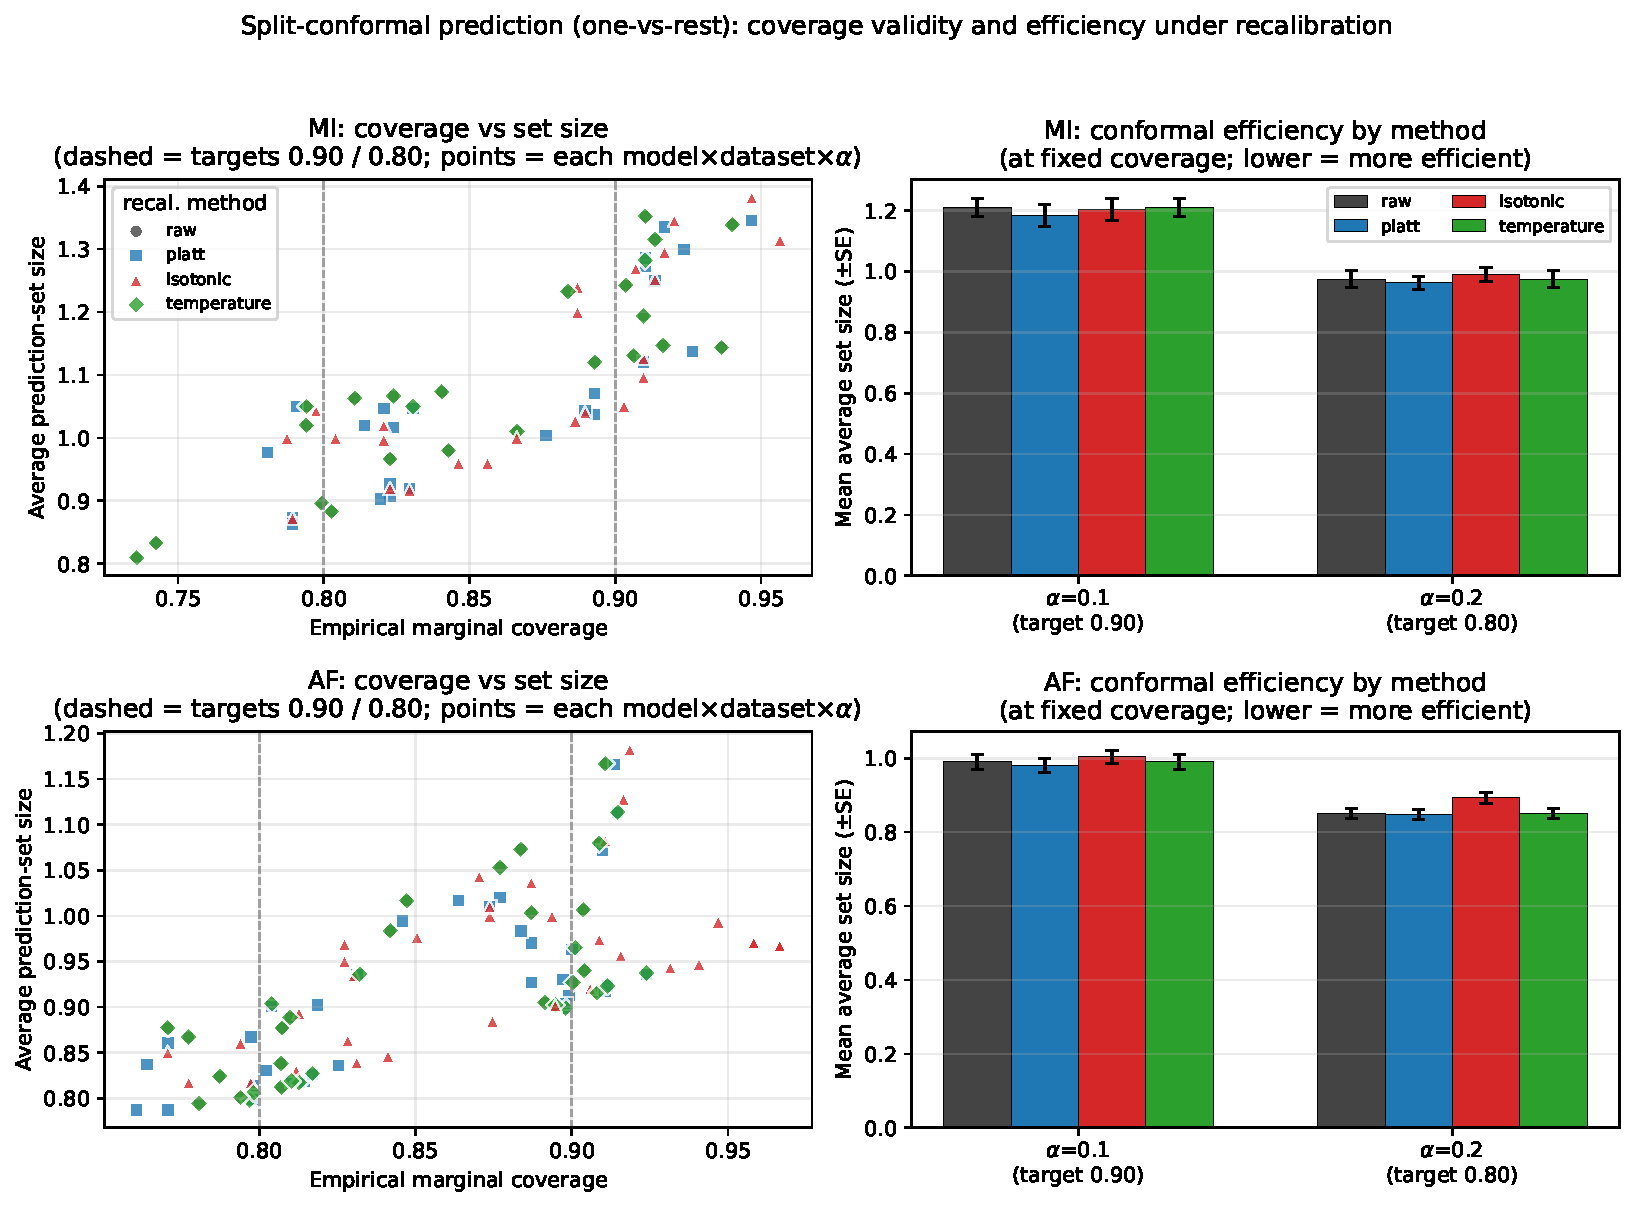
\includegraphics[width=0.96\linewidth]{figures/fig_conformal.pdf}
  \caption{Split-conformal prediction for the MI and AF endpoints: empirical coverage vs.\
    average set size by method. All methods attain target coverage; Platt is most efficient.}
  \label{fig:conformal}
\end{figure}

\subsection{Expanded Clinical Decision-Curve Analysis}
\label{sec:extended-dca}

We extend decision-curve analysis from a single curve to MI (PTB-XL, MIMIC-IV-ECG) and AF
(CODE-15\%, CPSC2018, MIMIC-IV-ECG) for all models, integrating net benefit over clinically
plausible threshold ranges (Figures~\ref{fig:dca-mi}--\ref{fig:dca-af}). Every model delivers
positive integrated net benefit above treat-all at MI thresholds (e.g.\ ST-MEM PTB-XL
$+0.027$; net benefit $+0.046$ at $t{=}0.15$), confirming that FM \emph{rankings} already
support useful decisions. For the rarer AF endpoint, integrated net benefit above treat-all is
large (e.g.\ $+0.19$ on CODE-15\%) because indiscriminate treat-all is costly at low
prevalence. Recalibration leaves integrated net benefit essentially unchanged (rank-preserving
methods cannot alter it, and isotonic changes it only marginally), but it is what makes the
\emph{probability} attached to each decision trustworthy---necessary when the numeric risk is
communicated or combined across models.

\begin{figure}[t]
  \centering
  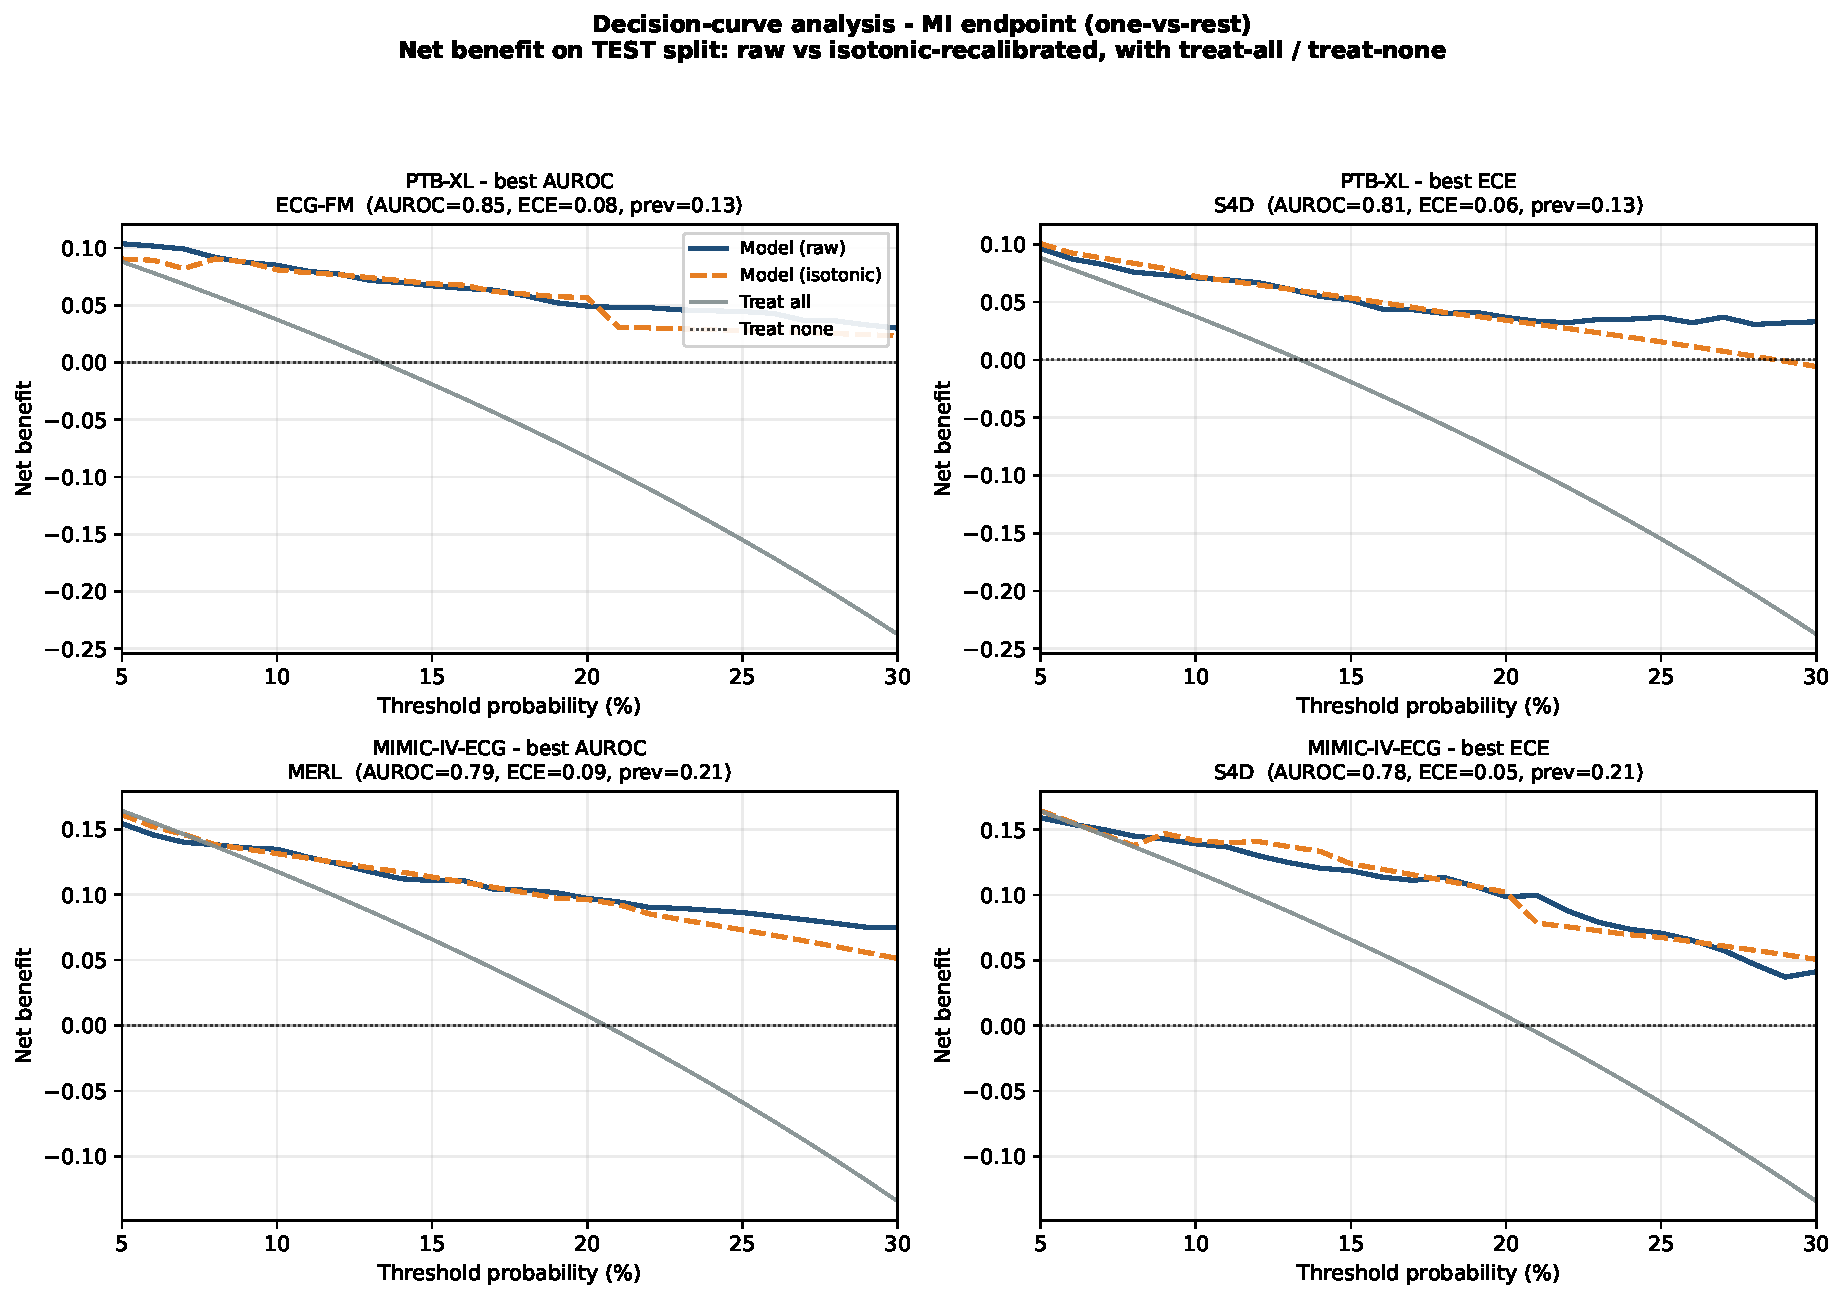
\includegraphics[width=0.96\linewidth]{figures/fig_dca_mi.pdf}
  \caption{Decision-curve analysis for MI on PTB-XL and MIMIC-IV-ECG, raw vs.\ isotonic, with
    treat-all/treat-none references.}
  \label{fig:dca-mi}
\end{figure}

\begin{figure}[t]
  \centering
  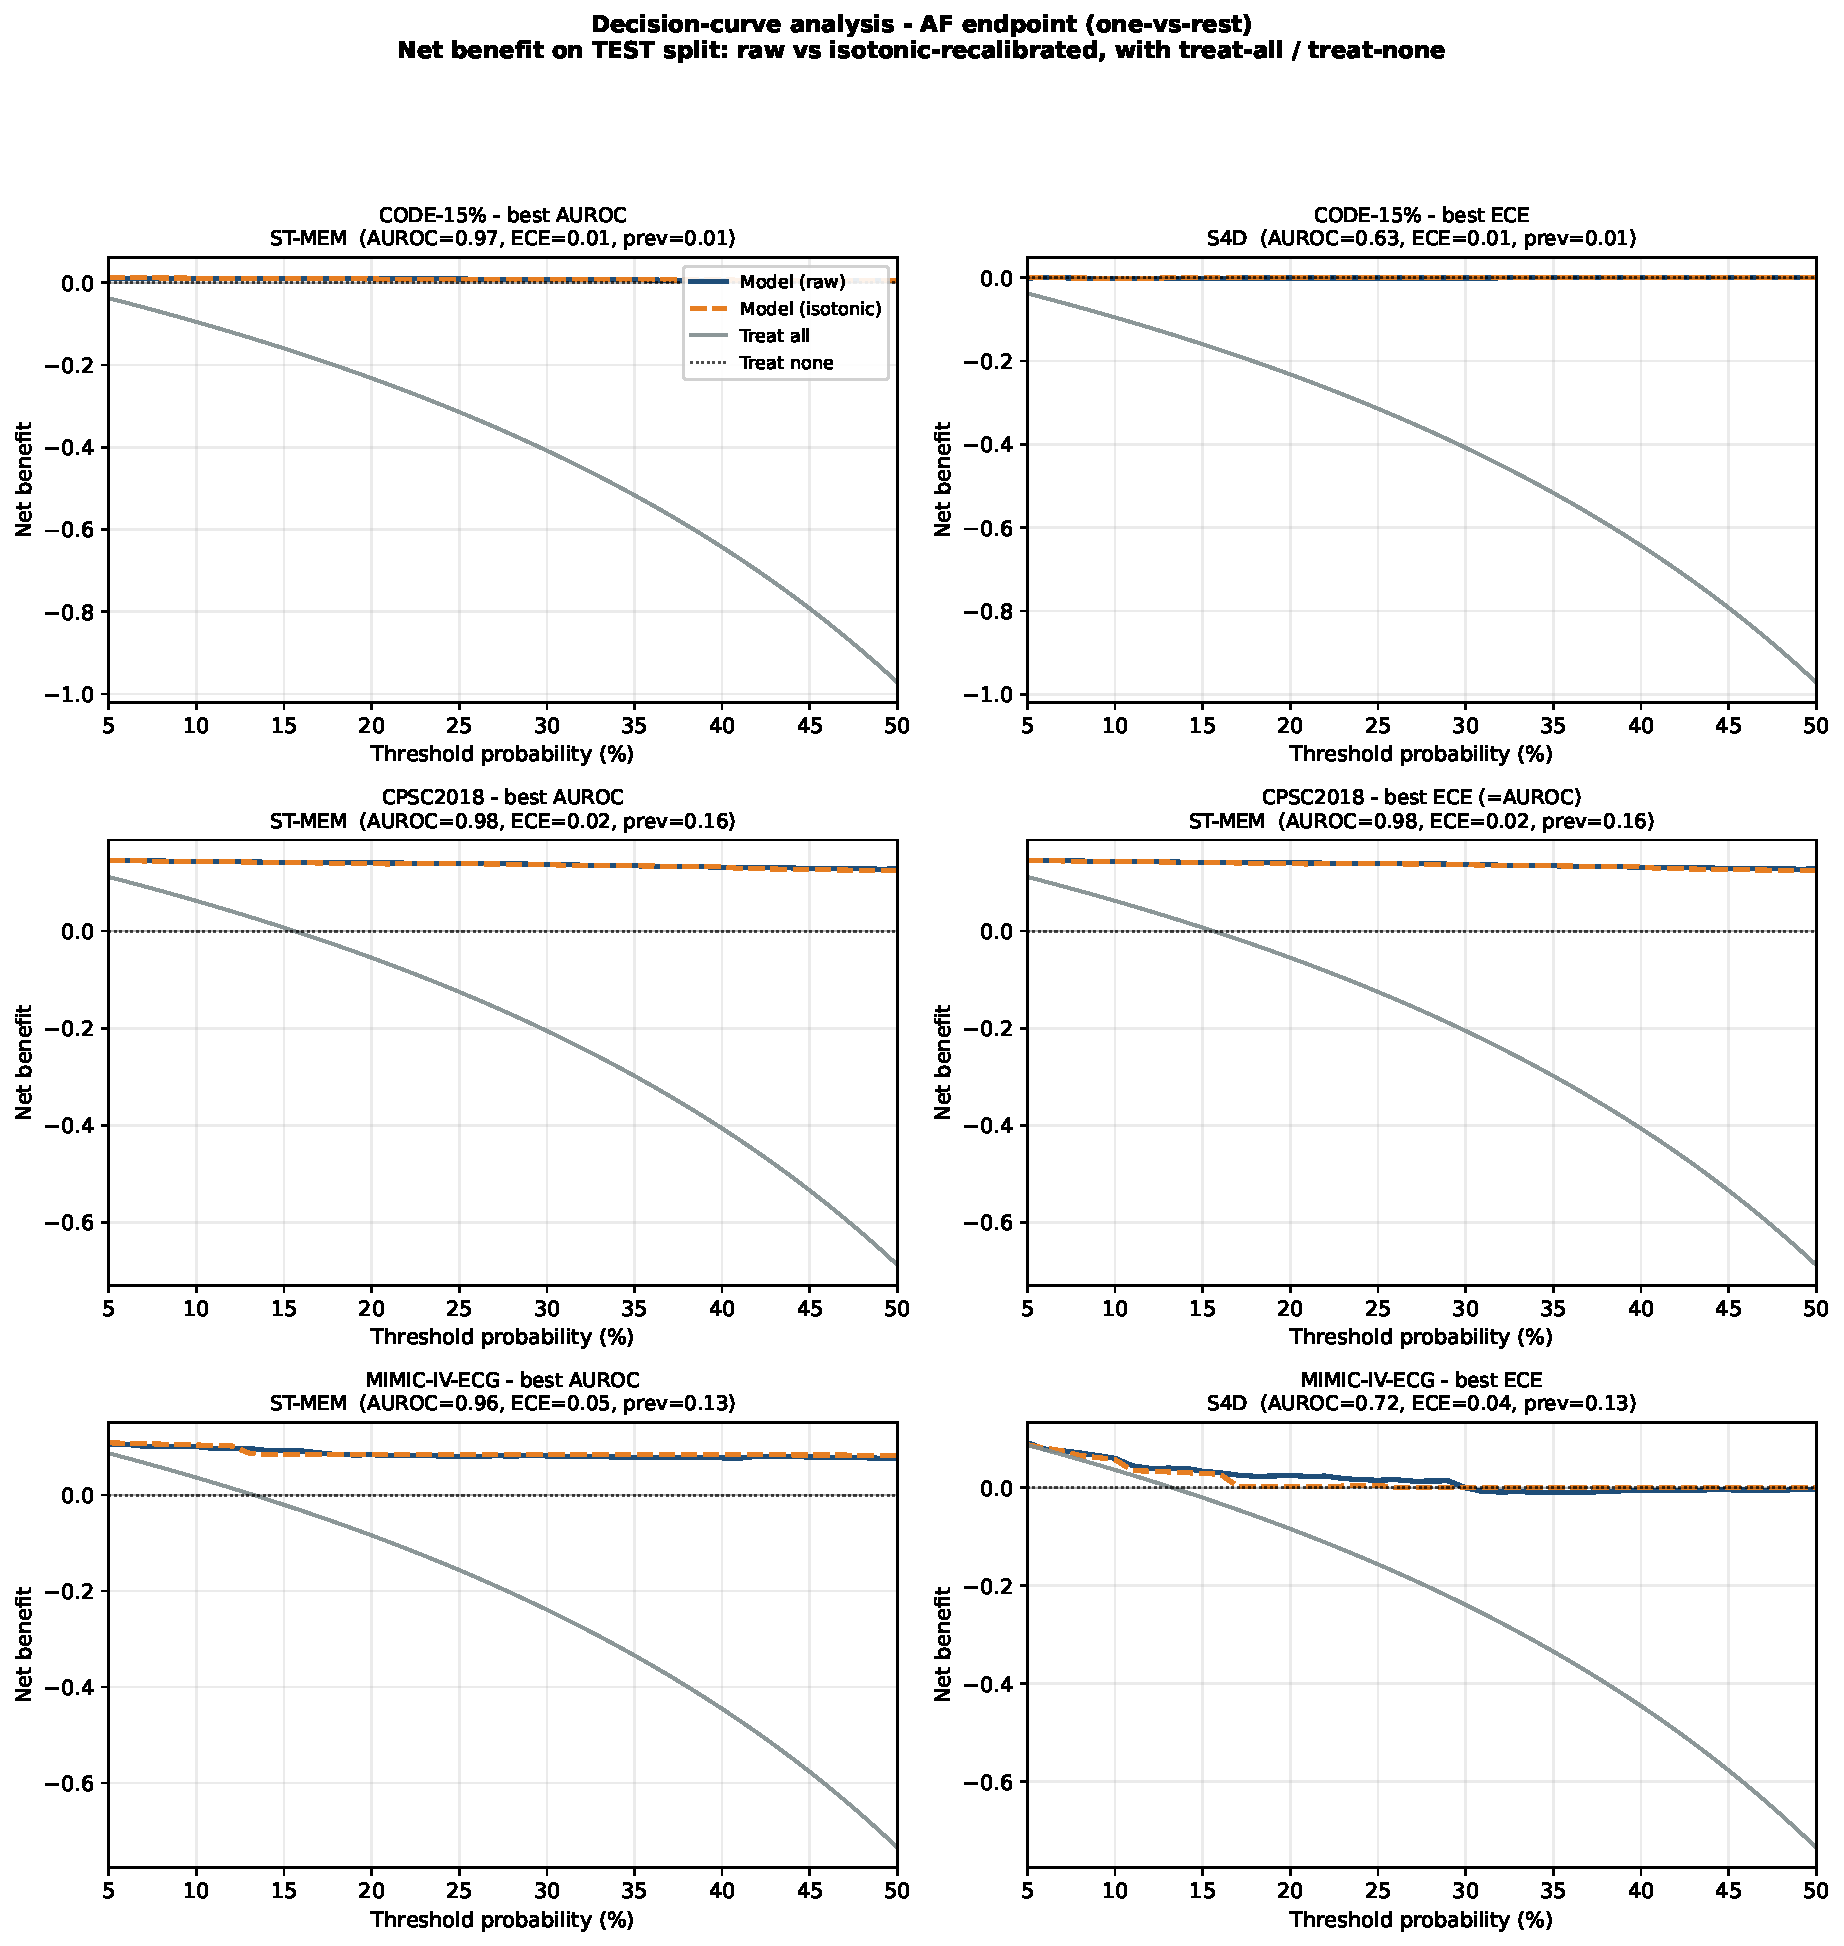
\includegraphics[width=0.96\linewidth]{figures/fig_dca_af.pdf}
  \caption{Decision-curve analysis for AF on CODE-15\%, CPSC2018, and MIMIC-IV-ECG.}
  \label{fig:dca-af}
\end{figure}

\subsection{Multi-Seed Robustness}
\label{sec:extended-robustness}

To show the headline conclusions are not split artefacts, we re-run the PTB-XL and
MIMIC-IV-ECG cells over 10 patient-level resplits (seeds 0--9; Table~\ref{tab:robustness},
Figure~\ref{fig:robustness}). The PTB-XL discrimination--calibration tradeoff is fully robust:
S4D has the lowest macro ECE of all six encoders in \textbf{10/10} seeds (mean gap $0.045$).
The within-domain finding is partially robust: ECG-FM trails MERL and ST-MEM in every seed,
but its AUROC ($0.792\pm0.015$) is \emph{statistically tied} with the supervised S4D baseline
($0.777\pm0.019$)---so we claim only that within-domain pretraining fails to beat the strong
self-supervised models, not that it underperforms a supervised baseline.

\begin{table}[t]
\centering
\caption{Multi-seed robustness (10 patient-level resplits, seeds 0--9): mean$\pm$std macro AUROC and ECE on the two multi-morbidity datasets. The PTB-XL discrimination--calibration tradeoff (S4D best-calibrated) holds in 10/10 seeds; ECG-FM trails MERL/ST-MEM on MIMIC in all seeds but is statistically tied with the S4D baseline.}
\label{tab:robustness}
\small
\begin{tabular}{llcc}
\toprule
Dataset & Model & AUROC (mean$\pm$std) & ECE (mean$\pm$std) \\
\midrule
  PTB-XL & MERL & 0.844$\pm$0.013 & 0.092$\pm$0.004 \\
   & ST-MEM & 0.852$\pm$0.015 & 0.119$\pm$0.009 \\
   & HuBERT-ECG & 0.801$\pm$0.018 & 0.141$\pm$0.009 \\
   & ECGFM-KED & 0.778$\pm$0.018 & 0.086$\pm$0.009 \\
   & ECG-FM & 0.812$\pm$0.015 & 0.100$\pm$0.010 \\
   & S4D & 0.785$\pm$0.021 & 0.062$\pm$0.004 \\
  \midrule
  MIMIC-IV-ECG & MERL & 0.882$\pm$0.012 & 0.063$\pm$0.004 \\
   & ST-MEM & 0.864$\pm$0.013 & 0.077$\pm$0.005 \\
   & HuBERT-ECG & 0.835$\pm$0.013 & 0.090$\pm$0.007 \\
   & ECGFM-KED & 0.744$\pm$0.018 & 0.066$\pm$0.006 \\
   & ECG-FM & 0.792$\pm$0.015 & 0.078$\pm$0.003 \\
   & S4D & 0.777$\pm$0.019 & 0.046$\pm$0.004 \\
\bottomrule
\end{tabular}
\end{table}

\begin{figure}[t]
  \centering
  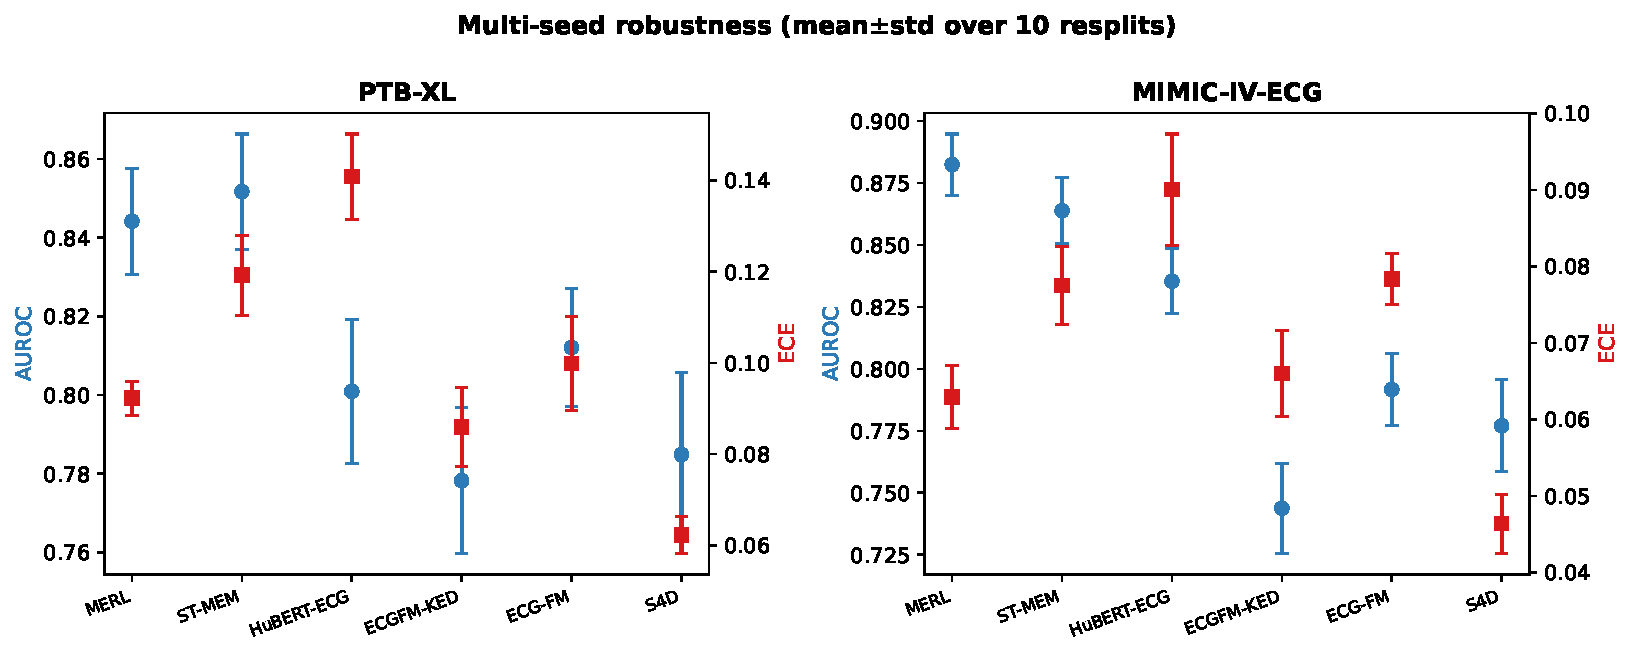
\includegraphics[width=0.96\linewidth]{figures/fig_robustness.pdf}
  \caption{Macro AUROC (blue) and ECE (red) as mean$\pm$std over 10 resplits, PTB-XL and
    MIMIC-IV-ECG. Rankings on both axes are stable.}
  \label{fig:robustness}
\end{figure}

\subsection{Mechanistic Regression: What Drives Miscalibration?}
\label{sec:extended-mechanistic}

To move beyond scatter plots we regress per-class ECE on candidate drivers across all
evaluated class-cells (OLS, $n{=}149$, $R^2{=}0.85$; Figure~\ref{fig:mechanistic}). Controlling
for everything else, \textbf{dataset/task structure dominates}: relative to PTB-XL, ECE is
lower by $0.074$ (CODE-15\%) and $0.076$ (CPSC2018) (both CIs exclude 0)---the multi-label
PTB-XL task is intrinsically harder to calibrate. \textbf{Masked-prediction pretraining}
independently raises ECE ($+0.044$ vs.\ contrastive, significant), while the
\textbf{supervised} objective lowers it ($-0.018$). At the class level, higher AUROC is
associated with slightly \emph{lower} ECE once dataset is controlled for---confirming that the
``rank well, calibrate poorly'' tradeoff is a model$\times$task phenomenon (the high-AUROC
foundation models on multi-label PTB-XL), not a universal law.

\begin{figure}[t]
  \centering
  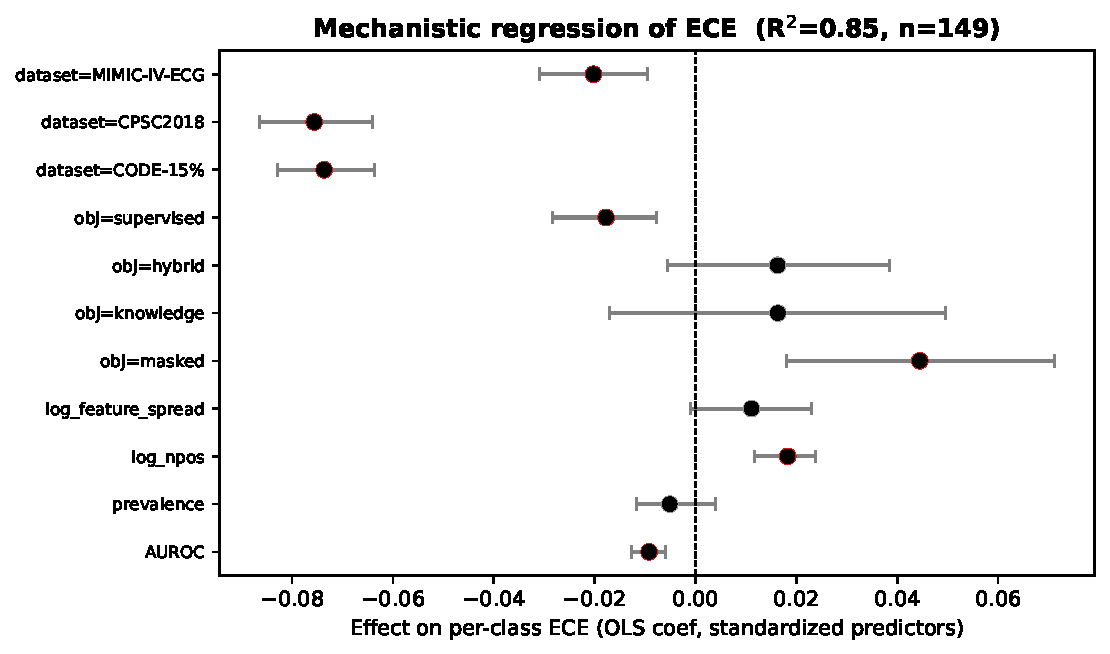
\includegraphics[width=0.82\linewidth]{figures/fig_mechanistic.pdf}
  \caption{OLS coefficients (standardized continuous predictors) for per-class ECE.
    Red = 95\% bootstrap CI excludes 0. Dataset and pretraining-objective effects dominate.}
  \label{fig:mechanistic}
\end{figure}

\subsection{Subgroup Calibration Across All Encoders}
\label{sec:extended-subgroup}

Extending the subgroup audit to all six encoders on PTB-XL (Figure~\ref{fig:subgroup-exp})
reveals a consistent age gradient: macro ECE rises from the $<$55 group to the $\geq$70 group
for \emph{every foundation model} (e.g.\ MERL $0.094\!\to\!0.143$, ST-MEM $0.111\!\to\!0.189$,
HuBERT-ECG $0.126\!\to\!0.183$), whereas the supervised S4D baseline stays flat
($0.117\!\to\!0.114$). Global calibration therefore hides a safety-relevant subgroup effect
specific to foundation-model representations: elderly patients receive the least reliable
probabilities from exactly the highest-AUROC models. This motivates subgroup-stratified
calibration auditing before deployment.

\begin{figure}[t]
  \centering
  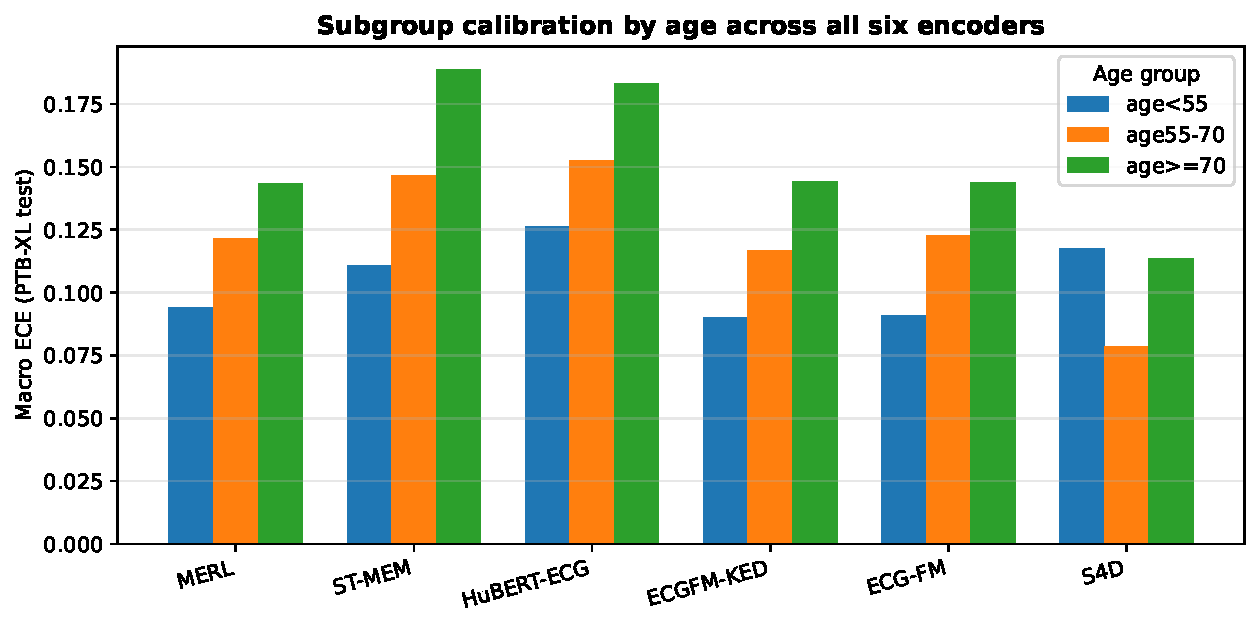
\includegraphics[width=0.92\linewidth]{figures/fig_subgroup_expanded.pdf}
  \caption{Macro ECE by age group across all six encoders (PTB-XL test). Foundation models
    degrade with age; the supervised baseline does not.}
  \label{fig:subgroup-exp}
\end{figure}

\section{Open-Source Tooling: ecg-audit}
\label{sec:open_source}

We release \texttt{ecg-audit}, a pip-installable Python package that provides
one-command calibration auditing for ECG foundation models, open-sourced at
\url{https://github.com/amensk/ecg-audit}. The package is implemented and unit-tested
(14 tests covering metrics, recalibration, and clinical utility); all analysis scripts are
available in \texttt{benchmark/} and the machine-readable result artifacts in \texttt{results/}.

\subsection{Package Description}

\texttt{ecg-audit} provides the following functionality:
\begin{itemize}
  \item \textbf{Calibration metrics}: ECE (equal-width and adaptive), SCE, Brier score,
    macro-averaged and per-class.
  \item \textbf{Recalibration methods}: temperature scaling, Platt scaling, isotonic
    regression, PhysioCalib (severity-weighted isotonic), MLP head.
  \item \textbf{Decision-curve analysis}: net benefit computation at arbitrary thresholds.
  \item \textbf{Subgroup analysis}: calibration by demographic subgroup.
  \item \textbf{Reliability diagrams}: publication-quality reliability diagram generation.
  \item \textbf{Leaderboard scaffold}: structured JSON output for community leaderboard
    population.
\end{itemize}

\subsection{CLI Example}

\begin{lstlisting}[language=bash, basicstyle=\ttfamily\small, frame=single]
# Audit predictions for three conditions
ecg-audit audit predictions.csv \
  --conditions MI,STTC,NORM \
  --output results/audit_report.json \
  --plot reliability_diagrams/

# Recalibrate with isotonic regression
ecg-audit recalibrate \
  --method isotonic \
  --cal-data cal_predictions.csv \
  --test-data test_predictions.csv \
  --output recalibrated_preds.csv
\end{lstlisting}

\subsection{Python API Example}

\begin{lstlisting}[language=python, basicstyle=\ttfamily\small, frame=single]
from ecg_audit import CalibrationAuditor, PhysioCalib

# Load predictions and labels
import numpy as np
probs = np.load("predictions.npy")   # (n, n_classes)
labels = np.load("labels.npy")       # (n, n_classes)
classes = ["NORM", "MI", "STTC", "CD", "HYP"]

# Audit raw calibration
auditor = CalibrationAuditor(classes=classes)
report = auditor.audit(probs, labels)
print(report.macro_ece, report.macro_sce)

# Apply PhysioCalib
weights = {"MI": 3.0, "STTC": 2.0, "CD": 1.5, "HYP": 1.2, "NORM": 0.5}
pc = PhysioCalib(severity_weights=weights)
pc.fit(probs_cal, labels_cal, classes)
probs_calibrated = pc.predict(probs_test)
\end{lstlisting}

\subsection{Leaderboard: Current State}

Table~\ref{tab:leaderboard} shows the current leaderboard state based on this benchmark.

\begin{table}[h]
\centering
\caption{ecg-audit leaderboard (current state), PTB-XL.
  $C(\alpha)=\alpha\cdot\mathrm{AUROC}+(1{-}\alpha)(1{-}\mathrm{ECE}/\mathrm{ECE}_{\max})$,
  $\alpha=0.7$, $\mathrm{ECE}_{\max}=0.136$. Rows sorted by $C(0.7)$ raw, descending.
  Note how recalibration reorders the table: ST-MEM is 5th on raw probabilities but 1st
  after isotonic recalibration.}
\label{tab:leaderboard}
\small
\begin{tabular}{lrrrrr}
\toprule
Model & PTB-XL & PTB-XL & CPSC & $C(0.7)$ & $C(0.7)$ \\
      & AUROC  & ECE    & AUROC & (raw)    & (post-iso) \\
\midrule
S4D        & 0.771 & 0.064 & 0.803 & \textbf{0.699} & 0.714 \\
MERL       & 0.828 & 0.087 & 0.910 & 0.688 & 0.771 \\
ECG-FM     & 0.815 & 0.088 & 0.847 & 0.676 & 0.774 \\
ECGFM-KED  & 0.769 & 0.079 & 0.821 & 0.664 & 0.771 \\
ST-MEM     & 0.838 & 0.124 & 0.950 & 0.614 & \textbf{0.789} \\
HuBERT-ECG & 0.787 & 0.136 & 0.876 & 0.551 & 0.763 \\
\bottomrule
\end{tabular}
\end{table}

\subsection{Reproducibility}

All frozen feature representations are cached as \texttt{.npy} files
(e.g.\ $2000\!\times\!512$ for MERL and $2000\!\times\!768$ for ST-MEM/HuBERT-ECG on PTB-XL;
$6877\!\times\!d$ for CPSC2018; ${\sim}8000\!\times\!d$ for the expanded CODE-15\% sample).
Primary benchmark outputs are in \texttt{results/benchmark\_v2\_results.json} (with bootstrap
CIs and per-class support) and \texttt{benchmark\_v2\_summary.csv}.
Analysis scripts are in \texttt{benchmark/} and cover feature extraction (including the
HuBERT-ECG \texttt{safetensors} loader), the consolidated benchmark, the CODE-15\% expansion,
feature geometry, Pareto analysis, decision-curve analysis, subgroup analysis,
calibration-set size curves, reliability diagrams, and PhysioCalib.

The leaderboard accepts new model entries without code changes. Any practitioner with a
predictions CSV can generate a leaderboard entry using the \texttt{ecg-audit submit} CLI
command, enabling community-driven calibration reporting for new ECG FM checkpoints.

\section{Discussion}
\label{sec:discussion}

\paragraph{Why the tradeoff disappears on CPSC2018.}
The most striking finding is the complete disappearance of the discrimination--calibration
tradeoff on CPSC2018. We attribute this to three structural differences from PTB-XL.
First, task type: CPSC2018 is a single-label 9-class task (each record has one dominant
arrhythmia), while PTB-XL is a 5-class multi-label task with correlated superclasses.
Multi-label calibration requires the linear probe to simultaneously assign valid probability
mass to correlated outputs --- a harder geometric problem that amplifies systematic
over- or under-confidence.
Second, class overlap: PTB-XL superclasses (e.g., MI and CD) frequently co-occur,
forcing the probe to partition probability across correlated classes. CPSC2018 classes
are more mutually exclusive.
Third, class prevalence: PTB-XL has highly variable class prevalences
(NORM: 48\%, HYP: 8\%), requiring the probe to operate at different operating points
for each class simultaneously. These structural differences suggest that calibration
auditing is most important for multi-label cardiac classification tasks.

\paragraph{Pretraining objective mechanism.}
MERL's underconfidence ($\text{SCE}=-0.003$ on PTB-XL) is consistent with the
documented behaviour of contrastive vision FMs~\citep{hekler2025beyond}. The mechanistic
interpretation is that contrastive objectives (InfoNCE) push representations apart to
maximise inter-class separation, producing a norm-uniform representation space with high
feature spread (std of L2 norms: 34.8 vs 0.23 for ST-MEM). When this spread representation
is projected through a linear probe, the probability outputs may be diffuse and underconfident
--- the probe cannot confidently assign high probabilities because the representation space
does not concentrate examples in tight class clusters.

The two masked-prediction models behave similarly in \emph{direction} but differ in
\emph{magnitude} of miscalibration. ST-MEM (masked patch reconstruction) and HuBERT-ECG
(masked hidden-unit prediction) both have near-zero SCE on PTB-XL ($-0.0001$ and $-0.0007$),
indicating no systematic over/under-confidence bias; yet both have the largest \emph{unsigned}
calibration error (ECE 0.124 and 0.136). Feature geometry explains the distinction: HuBERT-ECG
has the highest cosine class separation (0.046) of any model, and ST-MEM the second highest
(0.017), whereas MERL's separation is near zero (0.004). High class separation concentrates
predictions near 0/1, so when the empirical frequency disagrees the per-bin gap is large ---
producing high ECE even when the signed bias cancels out. Masked-prediction objectives thus
yield ``confidently wrong in both directions'' probabilities that recalibration is especially
effective at fixing (HuBERT-ECG ECE drops 71\% under isotonic).

ECGFM-KED (knowledge-enhanced, $+0.007$), ECG-FM (contrastive+generative, $+0.008$), and the
supervised S4D baseline ($+0.007$) are mildly overconfident on PTB-XL, suggesting that
decoder/generative and discriminative-supervised training shift calibration toward
overconfidence. This graded pattern --- contrastive underconfident, masked-prediction
neutral-but-high-ECE, knowledge/generative/supervised overconfident --- motivates further
study of how pretraining objectives shape probability calibration.

\paragraph{Recalibration recommendation.}
Based on the calsize analysis and DCA results, we summarise deployment recommendations:

\begin{center}
\begin{tabular}{lll}
\toprule
Calibration set size & Recommended method & Rationale \\
\midrule
$n_{\mathrm{cal}} < 63$      & Platt scaling          & Isotonic overfits; Platt is stable \\
$63 \leq n_{\mathrm{cal}} < 200$ & Isotonic regression    & Better ECE; crossover confirmed at $n=63$ \\
$n_{\mathrm{cal}} \geq 200$  & Isotonic regression    & Consistent 43--64\% ECE reduction \\
\bottomrule
\end{tabular}
\end{center}

Temperature scaling is not recommended for multi-label ECG tasks: it reduces ECE by only
11--38\% on PTB-XL, consistently worse than Platt scaling. The MLP head is unreliable
at $n_{\mathrm{cal}} < 100$, where it frequently underfits.

\paragraph{MIMIC-IV-ECG and within-domain pretraining.}
The MIMIC-IV-ECG results reveal a counter-intuitive finding: ECG-FM, which was pretrained
on MIMIC-IV-ECG data, achieves AUROC 0.771 on MIMIC-IV-ECG evaluation---below MERL (0.861)
and ST-MEM (0.854) in every resplit, and statistically tied with the supervised S4D baseline
(0.793; below S4D in only 2/10 seeds). This demonstrates that
backbone pretraining domain alignment is a necessary but not sufficient condition for
downstream linear-probe performance. The phenomenon likely arises because ECG-FM's hybrid
contrastive+generative pretraining objective optimises for self-supervised tasks (masked
prediction, contrastive similarity) that do not directly align with the
classification targets derived from machine-measurement reports. By contrast, MERL's
contrastive pretraining with clinical text descriptions may produce representations
more naturally aligned with the lexical structure of the machine measurement labels.
This has a practical implication: practitioners should not assume that a model pretrained
on their target cohort (e.g., in-house MIMIC-IV deployment) will automatically be the best
choice for a given classification task without linear-probe evaluation.

\paragraph{Cross-dataset calibration transfer.}
ECE varies by a factor of up to $10.3\times$ for the same model across datasets
(ST-MEM: CODE-15\% ECE 0.012 vs PTB-XL ECE 0.124). The MIMIC-IV-ECG dataset shows
intermediate calibration (ECE 0.033--0.061), suggesting that the calibration difficulty
correlates with label structure: binary single-class tasks (MIMIC machine labels, CODE-15\%)
are easier to calibrate than correlated multi-label superclasses (PTB-XL). Models calibrated
on CODE-15\% may be substantially miscalibrated on PTB-XL. This motivates re-calibration
on local data from the target deployment population.

\paragraph{Limitations.}
Six limitations bound this study's scope and generalisability.

\textbf{Frozen linear probes.} All evaluations use logistic linear probes on frozen
FM representations. Full fine-tuning may alter calibration --- potentially improving
or worsening it --- in ways not captured here. Calibration under fine-tuning is an
important open question.

\textbf{Sample sizes.} PTB-XL and MIMIC-IV-ECG use 2{,}000-record subsets and CODE-15\%
uses ${\sim}8{,}000$ records sampled across five HDF5 parts (chosen so that every rare
arrhythmia class clears the minimum-support threshold); the full datasets are larger still.
Larger samples may shift absolute ECE values, though the qualitative PTB-XL vs.\ arrhythmia
contrast is unlikely to reverse.

\textbf{HuBERT-ECG preprocessing.} HuBERT-ECG is included via its public \texttt{safetensors}
checkpoint. Following the authors' pipeline, the 12 leads are flattened into a single 1-D
sequence and decimated before encoding; this single-channel treatment differs from the
native multi-lead handling of the other encoders and may modestly affect its representations.

\textbf{ECGFM-KED architecture.} The partial architecture reconstruction (35 missing keys)
means ECGFM-KED results are lower bounds on true performance. The partial model likely
underestimates what the full ECGFM-KED would achieve.

\textbf{DCA scope.} The real DCA covers ST-MEM only.
Extending to MERL and ECG-FM is straightforward from cached features but not included.

\textbf{Subgroup analysis.} The age/sex subgroup analysis uses a re-trained probe
on the same 2,000-record sample; absolute calibration values are not directly
comparable to the main benchmark and the analysis is exploratory.

\paragraph{The ecg-audit package.}
The \texttt{ecg-audit} package provides these recalibration methods, plus the PhysioCalib
severity-weighted variant, as a one-command API. The package is installed and tested with
unit tests covering all recalibrators. The leaderboard scaffold allows the community to
populate calibration scores for additional FMs as checkpoints become available.

\section{Conclusion}
\label{sec:conclusion}

We present a systematic calibration audit of ECG foundation models: six encoders---five ECG
foundation models (MERL, ST-MEM, HuBERT-ECG, ECGFM-KED, ECG-FM) and a supervised S4D
baseline---across four datasets, with 23 of 24 model--dataset cells evaluated
(ECGFM-KED~$\times$~CODE-15\% excluded for a partial checkpoint), over 18{,}877 ECG records
(2{,}000 PTB-XL; 6{,}877 CPSC2018; 8{,}000 CODE-15\%; 2{,}000 MIMIC-IV-ECG) under
patient-level leakage-controlled splits with bootstrap confidence intervals.

\paragraph{Main findings.}
Four findings stand out. First, a consistent \textbf{discrimination--calibration tradeoff}
on PTB-XL: the five foundation models span AUROC 0.769--0.838 but all trail the supervised
S4D baseline's calibration (ECE 0.064), exceeding it by 0.015--0.072. ST-MEM achieves the
best discrimination (AUROC 0.838) but poor calibration (ECE 0.124), and HuBERT-ECG is the
worst calibrated (ECE 0.136)---a gap invisible to AUROC reporting but clinically significant.
Second, this tradeoff \textbf{disappears on arrhythmia datasets}: on CPSC2018
(ECE 0.023--0.051), CODE-15\% (ECE 0.010--0.032), and MIMIC-IV-ECG (ECE 0.043--0.106),
encoders are comparatively well-calibrated and ST-MEM leads discrimination. Task
structure---correlated multi-label vs.\ lower-co-occurrence endpoints---is the mediating factor. Third, \textbf{post-hoc
isotonic recalibration closes 43--71\% of the ECE gap} on PTB-XL (ST-MEM: $0.124\to0.044$;
HuBERT-ECG: $0.136\to0.040$) at only 0.5--1.7\% AUROC cost, and it reorders calibration-aware
model selection (ST-MEM moves from 5th to 1st on the $C(0.7)$ composite). Fourth,
\textbf{within-domain pretraining does not guarantee superiority}: ECG-FM, pretrained on
MIMIC-IV-ECG, achieves only AUROC 0.771 on MIMIC-IV-ECG---behind MERL (0.861) and ST-MEM
(0.854) in all 10 resplits, and no better than the supervised S4D baseline (0.793).
Cross-dataset ECE varies by up to ${\sim}6\times$ for
the same model, mandating per-deployment calibration audits.

\paragraph{A practical recipe.}
Beyond the audit we contribute \textbf{RankSafe-Cal}, which recovers most of isotonic's
calibration gain (PTB-XL macro ECE $0.097\!\to\!0.054$; on MIMIC it beats unconstrained
isotonic) at roughly $6\times$ lower AUROC cost by certifying out-of-sample ranking loss
within a tolerance $\epsilon$. Cross-dataset transfer experiments show recalibration ports
successfully in only 9--42\% of endpoint/model pairs, so local re-calibration remains
necessary. Split-conformal prediction attains its $90\%$ coverage guarantee as a complement
to calibration, and decision-curve analysis confirms positive net benefit for MI and AF
endpoints. All headline conclusions hold across 10 patient-level resplits.

\paragraph{Clinical implication.}
Practitioners deploying ECG foundation models for multi-label risk stratification should
mandate calibration auditing alongside AUROC benchmarking. Raw foundation-model
probabilities can be unusable for threshold-based clinical decisions even when AUROC is
excellent; post-hoc recalibration with as few as 63 examples eliminates most of the
calibration gap. The large cross-dataset ECE variation (e.g., ST-MEM ECE 0.028 on
CODE-15\% vs.\ 0.124 on PTB-XL) means calibration audits must be conducted on locally
representative patient cohorts---not extrapolated from published benchmark datasets.

\paragraph{Pretraining objective signal.}
A graded signature emerges: MERL (contrastive InfoNCE) shows the strongest underconfidence
($\text{SCE}=-0.003$), masked-prediction models (ST-MEM, HuBERT-ECG) are near-neutral, and
knowledge-enhanced, hybrid, and supervised models are mildly overconfident
($+0.007$--$+0.008$), consistent with the documented underconfidence of
contrastive FMs. Feature geometry analysis shows that MERL's contrastive objective
produces extreme feature spread (std of L2 norms: 34.8) relative to masked-prediction
and supervised models. Notably, MERL achieves the best performance on MIMIC-IV-ECG
(AUROC 0.866, ECE 0.033) despite not being pretrained on that cohort.

\paragraph{Open problems.}
Three directions remain for future work. First, \textbf{fine-tuning calibration}: this
study evaluates frozen linear probes; full fine-tuning may alter calibration in complex
ways that require re-auditing. Second, \textbf{larger MIMIC-IV-ECG evaluation}: this
benchmark used 2{,}000 records; the full 800{,}035-record corpus with structured ICD-based
labels (rather than parsed machine-measurement reports) would further strengthen the MIMIC
conclusions. Third, \textbf{objective-controlled pretraining}: the graded calibration
signature across contrastive, masked-prediction, knowledge-enhanced, and generative
objectives motivates controlled experiments that vary only the pretraining objective to
establish causality.

\paragraph{Call to action.}
The \texttt{ecg-audit} package and all benchmark scripts are ready to run against new
checkpoints without modification. We invite the ECG AI community to submit calibration
results to the leaderboard, enabling cumulative evidence on which models can be safely
deployed as probability estimators in clinical cardiac decision support.


\bibliographystyle{plainnat}
\bibliography{references}

\appendix
\section{Artifact Provenance and Evidence Boundary}
\label{sec:appendix}
\sloppy

\subsection{Completed Real Benchmark}

The 24-cell benchmark in Table~\ref{tab:full-benchmark} (23 evaluated cells; ECGFM-KED
$\times$ CODE-15\% excluded) is fully executed from real ECG recordings. All numeric values
trace to \texttt{results/benchmark\_v2\_results.json} and its summary
\texttt{benchmark\_v2\_summary.csv}. Frozen feature representations for every model--dataset
combination are cached as \texttt{.npy} files. Headline AUROC and ECE values carry bootstrap
95\% confidence intervals (1{,}000 resamples). The real DCA uses actual ST-MEM linear-probe
predictions recovered from cached features (not reconstructed proxies), saved in
\texttt{results/stmem\_ptbxl\_mi\_predictions.npz}.

\subsection{Evidence Classes}

\begin{itemize}
  \item \textbf{Full benchmark} (23 cells, primary): MERL, ST-MEM, HuBERT-ECG, ECGFM-KED,
    ECG-FM, and S4D on PTB-XL (2{,}000 records), CPSC2018 (6{,}877), CODE-15\%
    (${\sim}8{,}000$, parts 0--4), and MIMIC-IV-ECG (2{,}000). Patient-level splits, frozen
    linear probes, Phase~A calibration, Phase~B recalibration, minimum-support filtering,
    and bootstrap CIs.
  \item \textbf{HuBERT-ECG}: loaded from the public \texttt{safetensors} checkpoint via the
    HuggingFace \texttt{AutoModel} interface; 12 leads flattened and decimated per the
    authors' pipeline; 768-d mean-pooled embeddings.
  \item \textbf{DCA} (ST-MEM PTB-XL MI): net benefit from actual predictions.
  \item \textbf{Subgroup analysis} (exploratory): re-trained probe; absolute values differ
    from the main benchmark.
  \item \textbf{Calibration-size curves}: from \texttt{h4\_size\_ablation\_pilot\_summary.csv};
    extrapolations to $n\!>\!203$ are power-law projections.
  \item \textbf{Feature geometry}: from cached \texttt{.npy} features with PTB-XL labels
    (five foundation models).
\end{itemize}

\subsection{Remaining Limitations}

\begin{itemize}
  \item \textbf{ECGFM-KED $\times$ CODE-15\%}: partial architecture load (35 missing keys);
    near-chance AUROC; excluded from CODE-15\% claims and Pareto analysis. ECGFM-KED is
    retained on PTB-XL, CPSC2018, and MIMIC-IV-ECG.
  \item \textbf{Frozen probes only}: fine-tuning calibration is not evaluated.
  \item \textbf{MIMIC-IV-ECG labels}: parsed from machine-measurement reports on a
    2{,}000-record subset; LBBB falls below minimum support. Structured ICD-based labels on
    the full corpus are future work.
  \item \textbf{HuBERT-ECG preprocessing}: the authors' single-channel lead-flattening
    differs from the native multi-lead handling of the other encoders.
  \item \textbf{DCA scope}: real predictions for ST-MEM only; other models require re-running
    their probes from cached features.
  \item \textbf{PhysioCalib}: null finding at $n_\mathrm{cal}=297$; needs
    $n_\mathrm{cal}\!>\!500$ (estimated) for reliable minority-class improvement.
\end{itemize}

\subsection{Primary Artifact Paths}

\begin{itemize}
  \item \texttt{results/benchmark\_v2\_results.json} --- all 23 benchmark cells with CIs and
    per-class support; \texttt{benchmark\_v2\_summary.csv} --- flat summary.
  \item \texttt{results/features\_*.npy} --- cached frozen features for all six encoders on
    all four datasets (incl.\ HuBERT-ECG and MIMIC-IV-ECG); the \texttt{\_D3exp} suffix marks
    the expanded CODE-15\% sample.
  \item \texttt{results/pareto\_analysis\_v2.json} --- Pareto fronts and composite scores.
  \item \texttt{results/stmem\_ptbxl\_mi\_predictions.npz} --- real DCA predictions.
  \item Derived analyses in \texttt{results/}: \texttt{feature\_geometry.json},
    \texttt{dca\_results.json}, \texttt{subgroup\_results.json}, and
    \texttt{physio\_calib\_results.json}.
  \item \texttt{results/h4\_size\_ablation\_pilot\_summary.csv} --- calsize ablation.
\end{itemize}


\end{document}
